%%% The main file. It contains definitions of basic parameters and includes all other parts.

%% Settings for single-side (simplex) printing
% Margins: left 40mm, right 25mm, top and bottom 25mm
% (but beware, LaTeX adds 1in implicitly)
\documentclass[12pt,a4paper]{report}
\setlength\textwidth{145mm}
\setlength\textheight{247mm}
\setlength\oddsidemargin{15mm}
\setlength\evensidemargin{15mm}
\setlength\topmargin{0mm}
\setlength\headsep{0mm}
\setlength\headheight{0mm}
% \openright makes the following text appear on a right-hand page
\let\openright=\clearpage

%% Settings for two-sided (duplex) printing
% \documentclass[12pt,a4paper,twoside,openright]{report}
% \setlength\textwidth{145mm}
% \setlength\textheight{247mm}
% \setlength\oddsidemargin{14.2mm}
% \setlength\evensidemargin{0mm}
% \setlength\topmargin{0mm}
% \setlength\headsep{0mm}
% \setlength\headheight{0mm}
% \let\openright=\cleardoublepage

%% Generate PDF/A-2u
\usepackage[a-2u]{pdfx}

\usepackage[T1]{fontenc}
%% Character encoding: usually latin2, cp1250 or utf8:
\usepackage[utf8]{inputenc}

%% Prefer Latin Modern fonts
\usepackage{lmodern}

%% Further useful packages (included in most LaTeX distributions)
\usepackage{amsmath}        % extensions for typesetting of math
\usepackage{amsfonts}       % math fonts
\usepackage{amsthm}         % theorems, definitions, etc.
\usepackage{bbding}         % various symbols (squares, asterisks, scissors, ...)
\usepackage{bm}             % boldface symbols (\bm)
\usepackage{graphicx}       % embedding of pictures
\usepackage{fancyvrb}       % improved verbatim environment
\usepackage{natbib}         % citation style AUTHOR (YEAR), or AUTHOR [NUMBER]
\usepackage[nottoc,notlof,notlot]{tocbibind} % makes sure that bibliography and the lists
			    % of figures/tables are included in the table
			    % of contents

\usepackage{dcolumn}        % improved alignment of table columns
\usepackage{booktabs}       % improved horizontal lines in tables
\usepackage{paralist}       % improved enumerate and itemize
\usepackage{xcolor}         % typesetting in color

%%% Custom packages
\usepackage{enumitem}
\usepackage{ragged2e}
%\usepackage{todonotes}
\usepackage[font=small,labelfont=bf]{caption}
\usepackage{multirow}
\usepackage{multicol}
\usepackage{siunitx}
\usepackage{etoolbox}
\usepackage{scrextend}

\usepackage{tikz}
\usetikzlibrary{
    calc,
    decorations.markings,
    math,
    matrix,
    chains,
    positioning,
    arrows,
    shapes,
    decorations.pathreplacing,
    arrows.meta,
    shapes.multipart
}
\usepackage{pgfplots}
\pgfplotsset{compat=newest}

\usepackage{graphbox} % enable \includegraphics[align=c]{...}
\usepackage{setspace}

\gappto{\UrlBreaks}{\UrlOrds}



%%% Basic information on the thesis

% Thesis title in English (exactly as in the formal assignment)
\def\ThesisTitle{Deep Learning-Based Approaches for Shot Transition Detection and\linebreak[4] Known-Item Search in Video}

% Author of the thesis
\def\ThesisAuthor{Bc. Tomáš Souček}

% Year when the thesis is submitted
\def\YearSubmitted{2020}

% Name of the department or institute, where the work was officially assigned
% (according to the Organizational Structure of MFF UK in English,
% or a full name of a department outside MFF)
\def\Department{Department of Software Engineering}

% Is it a department (katedra), or an institute (ústav)?
\def\DeptType{Department}

% Thesis supervisor: name, surname and titles
\def\Supervisor{doc. RNDr. Jakub Lokoč, Ph.D.}

% Supervisor's department (again according to Organizational structure of MFF)
\def\SupervisorsDepartment{Department of Software Engineering}

% Study programme and specialization
\def\StudyProgramme{Computer Science}
\def\StudyBranch{Artificial Inteligence}

% An optional dedication: you can thank whomever you wish (your supervisor,
% consultant, a person who lent the software, etc.)
\def\Dedication{%
Hereby, I would like to thank my supervisor doc. RNDr. Jakub Lokoč, Ph.D. for his
valuable advice, suggestions, and support he gave me. I am also thankful he enabled me to present the work at international conferences.\\[6pt]

\noindent
Furthermore, I thank the Department of Software Engineering for providing me almost limitless GPU resources for my research.
}

% Abstract (recommended length around 80-200 words; this is not a copy of your thesis assignment!)
\def\Abstract{%
Video retrieval represents a challenging problem with many caveats and sub-problems. This thesis focuses on two of these sub-problems, namely shot transition detection and text-based search. In the case of shot detection, many solutions have been proposed over the last decades. Recently, deep learning-based approaches improved the accuracy of shot transition detection using 3D convolutional architectures and artificially created training data, but one hundred percent accuracy is still an unreachable ideal. In this thesis we present a deep network for shot transition detection TransNet V2 that reaches state-of-the-art performance on respected benchmarks. In the second case of text-based search, deep learning models projecting textual query and video frames into a joint space proved to be effective for text-based video retrieval. We investigate these query representation learning models in a setting of known-item search and propose improvements for the text encoding part of the model.
}

% 3 to 5 keywords (recommended), each enclosed in curly braces
\def\Keywords{%
{deep learning}, {shot boundary detection}, {known-item search}, {representation learning}
}

%% The hyperref package for clickable links in PDF and also for storing
%% metadata to PDF (including the table of contents).
%% Most settings are pre-set by the pdfx package.
\hypersetup{unicode}
\hypersetup{breaklinks=true}

\pdfinfo{
   /Author (Bc. Tomas Soucek)
   /Title (Deep Learning-Based Approaches for Shot Transition Detection and Known-Item Search in Video)
   /Keywords (deep learning;shot boundary detection;known-item search;representation learning)
}


% Definitions of macros (see description inside)
%%% This file contains definitions of various useful macros and environments %%%
%%% Please add more macros here instead of cluttering other files with them. %%%

%%% Minor tweaks of style

% These macros employ a little dirty trick to convince LaTeX to typeset
% chapter headings sanely, without lots of empty space above them.
% Feel free to ignore.
\makeatletter
\def\@makechapterhead#1{
  {\parindent \z@ \raggedright \normalfont
   \Huge\bfseries \thechapter. #1
   \par\nobreak
   \vskip 20\p@
}}
\def\@makeschapterhead#1{
  {\parindent \z@ \raggedright \normalfont
   \Huge\bfseries #1
   \par\nobreak
   \vskip 20\p@
}}
\makeatother

% This macro defines a chapter, which is not numbered, but is included
% in the table of contents.
\def\chapwithtoc#1{
\chapter*{#1}
\addcontentsline{toc}{chapter}{#1}
}

% Draw black "slugs" whenever a line overflows, so that we can spot it easily.
%\overfullrule=1mm

%%% Macros for definitions, theorems, claims, examples, ... (requires amsthm package)

\theoremstyle{plain}
\newtheorem{thm}{Theorem}
\newtheorem{lemma}[thm]{Lemma}
\newtheorem{claim}[thm]{Claim}

\theoremstyle{plain}
\newtheorem{defn}{Definition}

\theoremstyle{remark}
\newtheorem*{cor}{Corollary}
\newtheorem*{rem}{Remark}
\newtheorem*{example}{Example}

%%% An environment for proofs

\newenvironment{myproof}{
  \par\medskip\noindent
  \textit{Proof}.
}{
\newline
\rightline{$\qedsymbol$}
}

%%% An environment for typesetting of program code and input/output
%%% of programs. (Requires the fancyvrb package -- fancy verbatim.)

\DefineVerbatimEnvironment{code}{Verbatim}{fontsize=\small, frame=single}

%%% The field of all real and natural numbers
\newcommand{\R}{\mathbb{R}}
\newcommand{\N}{\mathbb{N}}

%%% Useful operators for statistics and probability
\DeclareMathOperator{\pr}{\textsf{P}}
\DeclareMathOperator{\E}{\textsf{E}\,}
\DeclareMathOperator{\var}{\textrm{var}}
\DeclareMathOperator{\sd}{\textrm{sd}}

%%% Transposition of a vector/matrix
\newcommand{\T}[1]{#1^\top}

%%% Various math goodies
\newcommand{\goto}{\rightarrow}
\newcommand{\gotop}{\stackrel{P}{\longrightarrow}}
\newcommand{\maon}[1]{o(n^{#1})}
\newcommand{\abs}[1]{\left|{#1}\right|}
\newcommand{\dint}{\int_0^\tau\!\!\int_0^\tau}
\newcommand{\isqr}[1]{\frac{1}{\sqrt{#1}}}

%%% Various table goodies
\newcommand{\pulrad}[1]{\raisebox{1.5ex}[0pt]{#1}}
\newcommand{\mc}[1]{\multicolumn{1}{c}{#1}}

\newrobustcmd*{\bftabnum}{%
	\bfseries
	\sisetup{output-decimal-marker={\textbf{.}}}%
}

% Title page and various mandatory informational pages
\begin{document}
%%% Title page of the thesis and other mandatory pages

%%% Title page of the thesis

\pagestyle{empty}
\hypersetup{pageanchor=false}
\begin{center}

\centerline{\mbox{
\includegraphics[width=166mm]{logo-en.pdf}}}

\vspace{-8mm}
\vfill

{\bf\Large MASTER THESIS}

\vfill

{\LARGE\ThesisAuthor}

\vspace{15mm}

{\LARGE\bfseries\begin{spacing}{1.0}\ThesisTitle\end{spacing}}

\vfill

\Department

\vfill

{
\centerline{\vbox{\halign{\hbox to 0.45\hsize{\hfil #}&\hskip 0.5em\parbox[t]{0.45\hsize}{\raggedright #}\cr
Supervisor of the master thesis:&\Supervisor \cr
\noalign{\vspace{2mm}}
Study programme:&\StudyProgramme \cr
\noalign{\vspace{2mm}}
Study branch:&\StudyBranch \cr
}}}}

\vfill

% Zde doplňte rok
Prague \YearSubmitted

\end{center}

%\newpage

%%% Here should be a bound sheet included -- a signed copy of the "master
%%% thesis assignment". This assignment is NOT a part of the electronic
%%% version of the thesis. DO NOT SCAN.
%%% This is not a~part of the electronic version of the thesis, do not scan!}

%%% A page with a solemn declaration to the master thesis

\openright
\hypersetup{pageanchor=true}
\pagestyle{plain}
\pagenumbering{roman}
\vglue 0pt plus 1fill

\noindent
I declare that I carried out this master thesis independently, and only with the cited
sources, literature and other professional sources. It has not been used to obtain another
or the same degree.

\medskip\noindent
I understand that my work relates to the rights and obligations under the Act No.~121/2000 Sb.,
the Copyright Act, as amended, in particular the fact that the Charles
University has the right to conclude a license agreement on the use of this
work as a school work pursuant to Section 60 subsection 1 of the Copyright~Act.

\vspace{10mm}

\hbox{\hbox to 0.5\hsize{%
In Prague, July 30, 2020
\hss}\hbox to 0.5\hsize{%
%signature of the author
\hss}}

% \hbox{\hbox to 0.5\hsize{%
% In \hbox to 6em{\dotfill} date \hbox to 6em{\dotfill}
% \hss}\hbox to 0.5\hsize{\dotfill\quad}}
% \smallskip
% \hbox{\hbox to 0.5\hsize{}\hbox to 0.5\hsize{\hfil Author's signature\hfil}}

\vspace{20mm}
\newpage

%%% Dedication

\openright

\noindent
\Dedication

\vglue 0pt plus 1fill
\noindent
This research has been supported by Czech Science Foundation (GA\v{C}R) project 19-22071Y, GA UK project 1310920 and SVV project 260451.
\vspace{20mm}

\newpage

%%% Mandatory information page of the thesis

\openright

\vbox to 0.5\vsize{
\setlength\parindent{0mm}
\setlength\parskip{5mm}

Title:
\ThesisTitle

Author:
\ThesisAuthor

\DeptType:
\Department

Supervisor:
\Supervisor, \SupervisorsDepartment

Abstract:
\Abstract

Keywords:
\Keywords

\vss}

\newpage

\openright
\pagestyle{plain}
\pagenumbering{arabic}
\setcounter{page}{1}


%%% A page with automatically generated table of contents of the master thesis

\tableofcontents

%%% Each chapter is kept in a separate file
\chapter*{Introduction}
\addcontentsline{toc}{chapter}{Introduction}

% For humans, vision is the most important source of information hence it is no surprise that video is considered as the richest type of multimedia available.
For humans, vision plays the most important role in building representation of the surrounding environment. We rely on sight heavily -- some even estimate that information from our eyes accounts for eighty percent of stimuli from the environment. It is, therefore, no wonder that, with the help of cheap recording devices that everybody carries in their pockets, we have become obsessed with capturing what we see.

Smartphones enabled us to record every moment of our lives, and personal archives of photos and videos started growing rapidly. With the rise of social networks and the internet in general, we began not only capturing photos and videos but also sharing them online. In 2013 it was reported that just only Facebook's databases contained 250 billion photos with 350 million new photos added every day by its users\footnote{\url{https://www.theverge.com/2013/9/17/4741332}} -- a figure that has probably grown since. Video platform YouTube announced in 2019 that it had been receiving more than 500 hours of video every minute\footnote{\url{https://www.cnbc.com/2018/03/14/with-over-1-billion-users-heres-how-youtube-is-keeping-pace-with-change.html}}. To put that in context, humans live shorter lives than the length of videos uploaded to the service every day.
% the length of videos uploaded in a day exceeds the length of human life.

With such amount of multimedia being recorded, new problems and challenges arise. Given the enormous sizes of collections, it is impossible to sequentially browse through the data. Efficient methods for work with multimedia collections need to be utilized. The use-cases for these methods vary from a plethora of methods for searching and transcribing the content to the summarization of the individual parts of the collections \cite{zhang2019pegasus_textsum,Miech_2019_ICCV_HowTo100M,zhou2018deep_videosum}.
Multimedia in the collections are, however, usually not manually annotated, and contain only basic metadata such as date, time, and location, if any at all.

In recent years, thanks to deep learning, we have seen huge improvements in many areas, including automatic annotation of images, videos, and other types of multimedia. Yet video, one of the richest type of multimedia, still presents multiple challenges, such as its enormous size. Compared to other types of media like text, audio, or images, video sizes are whopping -- a short clip can easily require a hundred times as much space as a single image. Comparison is even starker in the case of audio and text. As the deep learning-based approaches usually require large datasets, applying deep learning on video-related tasks depends upon the collection of harder to obtain and more time consuming to annotate datasets when compared to their image counterparts. Furthermore, training of the models requires more computational power and time due to the increased dimensionality of the problem.

A popular approach to circumvent the need for large training datasets or lack of computational power in end-to-end deep learning is to decompose a problem into multiple sub-problems, solving each independently. In the video domain, that means, for example, to extract image features from each frame and train a model utilizing only the extracted features instead of the high dimensional frames themselves \cite{Miech_2019_ICCV_HowTo100M,XirongW2VVpp}. In the domain of self-driving cars, one can create a model predicting a depth map from multiple images \cite{Yin_2019_CVPR_HD3} and then another model for obstacle detection using the images enriched with their depth \cite{Qi_2018_CVPR_FrustumPointNets}. In text-based systems, it is not uncommon to build on top of Word2Vec-like \cite{word2vec} pre-trained embeddings instead of training embeddings from scratch \cite{Miech_2019_ICCV_HowTo100M,XirongW2VVpp}. In general, the less training data there is, the more likely there will be benefits to utilizing the multi-step approach.

Many video-related methods take the decomposition approach to an extreme by discarding any temporal information from a video and working only with single frames or simply averaging multiple frames' features \cite{Miech_2019_ICCV_HowTo100M,XirongW2VVpp}. Surprisingly, until very recently \cite{Miech_2020_CVPR}, these methods dominated many video related benchmarks, probably due to lack of annotated video data.
% Until very recently methods utilizing only individual video frames dominated many video related benchmarks due to lack of annotated video data.
Strangely, even with the introduction of large annotated video datasets \cite{Ray_2018_ECCV}, we do not see such a sharp boost in performance, which can be seen in the image domain. Some theorize it is in part due to vagueness and ambiguity of actions observed in videos. Action \textit{`playing tennis'} can for different people mean vastly different clips. TV broadcasts from Wimbledon, table tennis tournament with friends in a basement, a kid hitting a ball in a backyard, or a computer game are all valid alternatives. 
Even though there is also ambiguity between objects, it is usually less pronounced.

To overcome the ambiguity and to correct errors of automatic methods, there has been research in human-assisted approaches \cite{VBS2019_overview}. They revolve around assisted browsing in the collections by utilizing novel user interfaces \cite{DuaneGurrin_VirtualReality_LSC2018}, hierarchical collection maps \cite{KlausWikiView}, or iterative query refinement by positive and negative examples \cite{Exquisitor_VBS2020,SOMHunterVBS2020}.
However, a comparison of such approaches is difficult because a person needs to be present in the evaluation loop. In recent years competitions such as Video Browser Showdown (VBS) \cite{VBS2019_overview} or Lifelog Search Challenge (LSC)~\cite{LSC2020} emerged to accelerate research in human-assisted approaches, in particular in a task of known-item search.
The known-item search (KIS) task represents a situation where a user searches for a given item (usually an image or a segment from a video) in a large collection of data.
%, e.g. a personal photo or video collection. In case of video KIS task where an user searches for a short clip
With an increasing amount of multimedia content we generate, there is a wide range of image or video collections where know-item search scenario may play an important role -- a personal photo or video archive, footage from CCTV cameras, databases of news clips or medical videos to name a few.

% Over the years the mentioned competitions served as a stage for evaluation of state-of-the-art tools for know-item search.
Over the years, Video Browser Showdown served as a stage for an evaluation of many known-item search approaches in large video collections. These are important concepts mentioned by winning teams:
\begin{description}[labelwidth=1em, leftmargin=!]
	\item \textbf{Powerful query initialization.} It is beneficial to limit search space by an initial query that filters out most of the unrelated items or, with enough luck, immediately discovers the searched video segment. For many years, color \cite{BlazekAdam2015} or edge sketches were widely used; however, these are useful only if a user knows the exact visual representation of a searched scene. Further, with advances in deep learning, concept and text search replaced sketches as it is a more effective approach \cite{LokocVBS2020_VIRET, vitrivr2020}. Lastly, note that the initial query also plays an important role in many query refinement methods introduced in the next paragraph as they require negative but also positive samples, which are hard to gather without good initialization.
	% is used to gather positive examples for query refinement.
	% It is beneficial to start iterative search with high chance .
	% No matter what query refinement method is used, large collections require 
	% Large databases require a method to reduce focus to only a part of the collection. Text search, search by example but text search dominates. Also Filters.
	\item \textbf{Effective query refinement.} In large collections with a lot of similar content, it is unlikely that the searched scene will be found on the first try with a query. Many KIS tools support either assisted text query reformulation based on presented results or encourage users to select positive and negative examples to further narrow and rearrange the result set \cite{Exquisitor_VBS2020,SOMHunterVBS2020}. Also, `find similar' function is widely used to retrieve similar content from the whole collection \cite{LokocVBS2019_Nasnet, vitrivr2020} -- nowadays usually implemented as nearest-neighbor search in high-dimensional representations of the content computed by deep neural networks.
	% Recently Bayesian approach that displays images based on their probability given positive and negative samples proved to be useful.
	\item \textbf{Fast assisted browsing.} Browsing is utilized if a scene is not found using only the approaches mentioned above. %It is strongly tied to query refinement since the refinement commonly requires good results to start from.
	Good browsing approaches should exploit information from initial query results but also consider further exploration. Some methods of browsing involve computation of 2D image maps \cite{KlausVBS2019_sketchsearch, KlausWikiView}, and some utilize the power of virtual reality \cite{DuaneGurrin_VirtualReality_LSC2018}. Recently, Bayesian approach that samples images to display based on their probability proved to be successful \cite{SOMHunterVBS2020}.
	\item \textbf{Intuitive user interface.} The tools are operated by not only the authors but also by novice users. A cluttered user interface or hard-to-understand retrieval models result in lower performance of a tool when operated by novices.
\end{description}
%There is also another key part of all KIS tools -- key frame selection. It is not mentioned in related work much since collections used at competitions usually come with pre-selected set of key frames using some heuristics.
\begin{description}[labelwidth=1em, leftmargin=!]
	\item \textbf{Key frame selection.} In general, videos may be too long and may contain different unrelated scenes. Therefore, the search is often performed on shorter video segments. Usually, a segment of a video is represented by a single frame (keyframe). The selection of the segment and its keyframe can be performed by thresholding differences between (multiple) adjacent frames and their visual features \cite{V3C1dataset}. However, setting threshold too low results in oversampling, which increases database size and clutters result lists. Too high threshold causes some unique video segments to be missed. Recently more accurate shot boundaries, detected by deep learning-based methods \cite{LokocMM2019}, have been used instead of rather vaguely defined segments.
\end{description}
With these concepts in mind, at VBS 2019 \cite{VBS2019_overview} on V3C1 1000 hour dataset \cite{V3C1dataset}, the best performing teams of experts were able to solve all ten tasks where the search clip was played to an audience, and six out of ten tasks where only a textual description was available. At VBS 2020, on the same dataset, the best team in expert session solved five out of six visual tasks and eight out of ten textual tasks. For the next years, much bigger datasets are planned; however, given the rapid pace of innovation in deep learning and other related areas, we expect to see even better results in the foreseeable future.


% In general there are two approaches to deep leaenig mocels: use only raw data as an input and target task as an output or decompose problem into myultiple sub tasks and solve each indimendenty. In video it is extract image freatures from each frame, build model on top of the features only insyteaod of high dimensional frames. In conversational chatbots it is that we decode audio into text, then create reply and again generate sound. Even in malware detection we can either use the raw files directly or create handengeneerd features and train model on top of the features only. Ususally the larger the input the more likely end to end approchs fails ... more difficult problem - no training data -> the later approcha is used. In self driing cars use create depth map from images and use it together to detect objects....

% Therefore it is no surprise that video is considered as one of the richest type of multimedia. However the richness of videos comes at great cost -- size. Compared to other types of media such as text, audio or images, video sizes are whooping -- a short clip can easily require hundred times as much space as a single image. Comparison is even starker in case of audio and text. 
% It is therefore no wonder that until relative recent advances in video compression techniques and storage video could not compete with crispness and detail of images.
%To further complicate the matter, video search can be more abstract since actions such as `chopping some vegetable' or `walking along a river' are not as precisely defined compared to standard image search objectives such as `an orange' or `the Eiffel Tower'.


\section*{Our Contribution}
\addcontentsline{toc}{section}{Our Contribution}
In this thesis, we propose, implement, and evaluate new methods and improvements in two key areas of video retrieval. Namely a shot boundary detection and text search in video or image collections. For the shot boundary detection -- a task to detect continuous video sequence captured by a single camera -- we present a state-of-the-art method based on deep learning that outperforms both standard thresholding methods as well as more recent learning-based methods on multiple public benchmarks. For text search in video collections, we improve W2VV++~\cite{XirongW2VVpp} -- a model that computes the similarity between a text and video by projecting both modalities into joint vector space using a neural network. We enrich W2VV++ with a more powerful natural language model and discuss its greatly superior performance on some tasks while achieving a bit lower performance on others.

Our work is a culmination of many years of research primarily focused on known-item search in video collections. Some of the work presented in this thesis has been published at international conferences. Aside from the already published content, the thesis contains more detailed method descriptions as well as additional experiments and ablation studies, while other aspects of known-item search are mostly left out as the sole focus of the thesis is shot boundary detection and text search. The main publications regarding the content of the thesis are the following:
\begin{enumerate}
	\item \textbf{A framework for effective known-item search in video}~\cite{LokocMM2019}\\
	Full paper describing effective approaches to known-item search. The paper also introduces TransNet shot boundary detection network. Published at ACM International Conference on Multimedia 2019 (CORE A*).
	\item \textbf{TransNet: A deep network for fast detection of common shot transitions}~\cite{soucek2019transnet}\\
	Short paper slightly extending the version published at ACM Multimedia. Published on Arxiv.
	\item \textbf{A W2VV++ Case Study with Automated and Interactive Text-to-Video Retrieval}~\cite{W2VVppMM2020}\\
	Full paper studying W2VV++ query representation learning model \cite{XirongW2VVpp} in text-based video retrieval scenarios. The paper also introduces our BERT extension to the W2VV++ model. Accepted to ACM International Conference on Multimedia 2020 (CORE A*).
	\item \textbf{TransNet V2: An effective deep network architecture for fast shot transition detection}~\cite{soucek2020transnetv2}\\
	Short paper describing our TransNet V2 model.% In review for ACM International Conference on Multimedia 2020.
\end{enumerate}
We also list some of the author's publications in the field of known-item search:
\begin{enumerate}\setcounter{enumi}{4}
	\item \textbf{Interactive Video Retrieval in the Age of Deep Learning -- Detailed Evaluation of VBS 2019}~\cite{VBS2019_overview}\\
	Journal paper analyzing the results of VBS 2019. Published in IEEE Transactions on Multimedia (IF = 6.051).
	\item \textbf{VIRET: A video retrieval tool for interactive known-item\linebreak[4] search}~\cite{LokocICMR2019}\\
	Short paper presenting our VIRET tool and showing an analysis of interaction logs from VBS 2019. Published at ACM International Conference on Multimedia Retrieval 2019.
	\item \textbf{VIRET at Video Browser Showdown 2020}~\cite{LokocVBS2020_VIRET}\\
	Demo paper describing latest version of our retrieval tool. Published at ACM International Conference on Multimedia Modeling 2020.
\end{enumerate}
Other demo papers \cite{LokocVBS2019_Nasnet,LokocLSC2019} were published on the occasions of the VBS and LSC competitions at MMM and ACM ICMR respectively. Papers \textit{Revisiting SIRET Video Retrieval Tool}~\cite{LokocVBS2018} and \textit{Using an Interactive Video Retrieval Tool for LifeLog Data}~\cite{LokocLSC2018} were already presented in the author's bachelor thesis.

We proudly report that we achieved first and second place at VBS 2018 and VBS 2019 respectively. At VBS 2020, two tools \cite{LokocVBS2020_VIRET,SOMHunterVBS2020} using our shot boundary detection method and a simplification of the W2VV++ model, as reported in \cite{W2VVppMM2020}, achieved first and second place. Furthermore, we achieved third and second place at LSC 2018 and LSC 2019 respectively.


\section*{Thesis Structure}
\addcontentsline{toc}{section}{Thesis Structure}

The thesis is divided into two chapters. The first chapter introduces methods for shot boundary detection and presents TransNet -- a neural network for shot detection (Section \ref{sec:transnetv1}). Further in the chapter, significant improvements to TransNet are made, and a new network TransNetV2 is introduced (Section \ref{sec:transnetv2}). Finally, related works are reevaluated for a fair comparison with TransNetV2 in Section \ref{sec:transnetv2_evaluation}, and an ablation study is made. The second chapter introduces approaches towards text search in image and video collections, especially the W2VV++ model by Li et al. \cite{XirongW2VVpp} (Section \ref{sec:chap2relatedwork}), and our extension W2VV++BERT is presented in Section \ref{sec:chap2ourmethod}. Both models are thoroughly evaluated together with an ablation study in Section \ref{sec:chap2experiments}.

Source code for TransNetV2, including a version with a trained model for easy integration and reevaluation, training scripts, and dataset manipulation scripts are provided as an attachment to the thesis as well as available online at \url{https://github.com/soCzech/TransNetV2}. Source code for the W2VV++BERT network, together with trained weights and details for feature extraction, are also attached to the thesis as well as available online at \url{https://github.com/soCzech/w2vvpp_bert}.


\section*{Authorship}
\addcontentsline{toc}{section}{Authorship}

All experiments presented in this thesis have been conducted solely by the author of the thesis with the only exception of the original TransNet model, described in Section \ref{sec:transnetv1}, which has been created by Mgr. Jaroslav Moravec. However, further TransNet evaluations were done by the author of this thesis. Also, the model's description in Section \ref{sec:transnetv1} as well as the paper \textit{TransNet: A deep network for fast detection of common shot transitions}~\cite{soucek2019transnet} and corresponding sections of the paper \textit{A framework for effective known-item search in video}~\cite{LokocMM2019} were written by the author of this thesis with the help of his supervisor. TransNetV2 presented in Section \ref{sec:transnetv2} has been solely the author's work.

As the work presented in this thesis has been published at international conferences, some of the thesis' content may correspond to the author's publications listed above. All such possible correspondences were written by the author of this thesis with the help of his supervisor.

\chapter{Shot Boundary Detection}

Commonly, a video structure is as follows: The video is divided into scenes and each scene into one or more shots. A shot is a continuous frame sequence captured by a single camera action \cite{FormalStudyofSBD}. Some works introduce stories, that group semantically related scenes \cite{MethodsandChallengesinSBD}, or threads, that group similar shots, e.g. captured from the same camera point \cite{LearningContextualThreadModelSceneSegmentation}. Shots are, however, the most studied and the most used since shot detection is considered a fundamental step in video analysis. Information about shots is being exploited in video summarization \cite{Zhao_2018_CVPR}, video retrieval for advanced browsing and filtering \cite{LokocVBSJournal2018}, or even content-based copy detection \cite{Fuzzycolorhistogram}. However, information about the transitions is not available in the video format. Therefore, automated shot boundary detection methods need to be employed.

% A popular way to structure a video is by making use of a shot composition, where shots are delimited by transitions. Since information about the transitions is not available in the video format, automated shot boundary detection is an important step for video management and retrieval systems. For example, information about shots can be employed for video summarization, advanced browsing and filtering in known-item search tasks \cite{CobarzanSBHBLVB17,LokocBSMA18,Lokoc2019}.
% Shot changes can be either immediate (hard cuts) or gradual, the later spanning from basic linear interleaving of two shots over a certain number of video frames to more exotic geometric transformations from one shot to another one.
Any successful method must take into account that shot changes can be either immediate (hard cuts) or gradual. Common types of gradual transitions include dissolves (interleaving of two shots over a certain number of video frames), fade-ins and fade-outs (also considered as special types of dissolves where one shot is a blank image of a single color) and wipes (one shot slides from a side on top of the other shot). However, there are also many more exotic geometric transformations from one shot to another one.
%The later spanning from basic dissolves (interleaving of two shots over a certain number of video frames) to more exotic geometric transformations from one shot to another one. 
To make matters worse, shot boundary detectors must distinguish between shot transitions and sudden changes in a video caused by flashing light or partial occlusion of the scene by an object passing closer to the camera. Fast camera motion or motion of an object in the scene should also not be mistaken for a shot transition. This may indicate that some semantic representation of a scene is necessary to correctly segment a video.

Lastly, in some cases, a shot boundary is not a well-defined concept and question whether there is a transition may be subjective. Here we list some ambiguous cases and leave it for the reader to decide whether it should be a transition or not. Is a moment when captions are displayed at the end of a movie a transition? What if they raise from the bottom of the frame? A camera slowly enters a dark room -- is it fade-out? Newscast with two reporters side-by-side -- what if there is cut in a window of one reporter? Yet, with these examples, we only scratch the surface of the problem. Therefore, when used in the wild, shot boundary detection methods need to be tuned to eliminate these ambiguities based on a particular task at hand. % in case of computer generated content there are even more ambiguous scenarios.

% - news bar stays while shot changes, news bar changes while shot stays the same
% - what if the news two reporters side by side, at one cut is made, what if cut is performed in small picture-in-picture overlay?
% - camera enters dark room, is it fade out?
% - are captions shot transitions?




\section{Related work}

There has been a lot of research in shot boundary detection methods. The methods range from the most basic ones, that utilize only pixel-wise differences \cite{zhang93} effective for cut detection in stationary shots with a small number of moving objects, to more robust techniques that have been developed in the last years. Firstly, we list some of the `standard' methods not based on neural networks, further in the section deep learning approaches are discussed. For a more complete overview of the `standard' methods, we point the reader to some of many review studies available~\cite{MethodsandChallengesinSBD}.

\begin{figure}
    \centering
    \begin{tikzpicture}[
    font=\sffamily\scriptsize,
    table/.style={
        matrix of nodes,
        row sep=-\pgflinewidth,
        column sep=-\pgflinewidth,
        nodes={
            rectangle,
            draw=black,
            align=center,
            inner sep=0pt,
            minimum height=0.35cm,
            text width=0.35cm,
        },
        font=\sffamily\tiny,
        nodes in empty cells,
    }]
    \definecolor{Xcolor}{RGB}{0,0,0}
    
\node[inner sep=0pt] at (-4,0)
{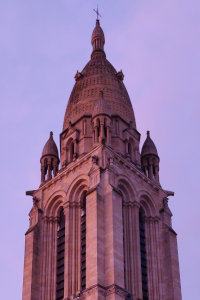
\includegraphics[align=c,width=.2\textwidth]{img/transnetv2/IMG_20200307_191029_edited.jpg}};

    \matrix [table] at (0,0){
|[fill=Xcolor!  16]| & |[fill=Xcolor!   8]| & |[fill=Xcolor!   0]| & |[fill=Xcolor!   0]| & |[fill=Xcolor!   0]| & |[fill=Xcolor!   0]| & |[fill=Xcolor!   0]| & |[fill=Xcolor!   0]| \\
|[fill=Xcolor!  13]| & |[fill=Xcolor!  28]| & |[fill=Xcolor!   5]| & |[fill=Xcolor!   0]| & |[fill=Xcolor!   0]| & |[fill=Xcolor!   0]| & |[fill=Xcolor!   0]| & |[fill=Xcolor!   0]| \\
|[fill=Xcolor!   7]| & |[fill=Xcolor!  32]| & |[fill=Xcolor!  38]| & |[fill=Xcolor!   5]| & |[fill=Xcolor!   1]| & |[fill=Xcolor!   0]| & |[fill=Xcolor!   0]| & |[fill=Xcolor!   0]| \\
|[fill=Xcolor!   1]| & |[fill=Xcolor!  19]| & |[fill=Xcolor!  44]| & |[fill=Xcolor!  30]| & |[fill=Xcolor!   6]| & |[fill=Xcolor!   2]| & |[fill=Xcolor!   0]| & |[fill=Xcolor!   0]| \\
|[fill=Xcolor!   0]| & |[fill=Xcolor!   4]| & |[fill=Xcolor!  27]| & |[fill=Xcolor!  26]| & |[fill=Xcolor!   8]| & |[fill=Xcolor!   7]| & |[fill=Xcolor!   3]| & |[fill=Xcolor!   0]| \\
|[fill=Xcolor!   0]| & |[fill=Xcolor!   0]| & |[fill=Xcolor!   7]| & |[fill=Xcolor!  29]| & |[fill=Xcolor!  12]| & |[fill=Xcolor!   6]| & |[fill=Xcolor!  29]| & |[fill=Xcolor! 100]| \\
|[fill=Xcolor!   0]| & |[fill=Xcolor!   0]| & |[fill=Xcolor!   0]| & |[fill=Xcolor!  11]| & |[fill=Xcolor!  19]| & |[fill=Xcolor!   2]| & |[fill=Xcolor!   5]| & |[fill=Xcolor!  35]| \\
|[fill=Xcolor!   0]| & |[fill=Xcolor!   0]| & |[fill=Xcolor!   0]| & |[fill=Xcolor!   0]| & |[fill=Xcolor!   1]| & |[fill=Xcolor!   0]| & |[fill=Xcolor!   0]| & |[fill=Xcolor!   0]| \\
    };
    
    \node[] at (0, 1.7) {\footnotesize RGB Histogram};
    \node[rotate=90] at (-1.7, 0) {Red};
    \node[] at (0, -1.7) {Blue};
    
        \matrix [table] at (4,0){
|[fill=Xcolor!   0]| & |[fill=Xcolor!   0]| & |[fill=Xcolor!   7]| & |[fill=Xcolor!  17]| & |[fill=Xcolor!  10]| & |[fill=Xcolor!   6]| & |[fill=Xcolor!   2]| & |[fill=Xcolor!   1]| \\
|[fill=Xcolor!   0]| & |[fill=Xcolor!   0]| & |[fill=Xcolor!   0]| & |[fill=Xcolor!   0]| & |[fill=Xcolor!   0]| & |[fill=Xcolor!   0]| & |[fill=Xcolor!   0]| & |[fill=Xcolor!   0]| \\
|[fill=Xcolor!   0]| & |[fill=Xcolor!   0]| & |[fill=Xcolor!   0]| & |[fill=Xcolor!   0]| & |[fill=Xcolor!   0]| & |[fill=Xcolor!   0]| & |[fill=Xcolor!   0]| & |[fill=Xcolor!   0]| \\
|[fill=Xcolor!   0]| & |[fill=Xcolor!  36]| & |[fill=Xcolor! 100]| & |[fill=Xcolor!   4]| & |[fill=Xcolor!   7]| & |[fill=Xcolor!   4]| & |[fill=Xcolor!   1]| & |[fill=Xcolor!   1]| \\
|[fill=Xcolor!   0]| & |[fill=Xcolor!  54]| & |[fill=Xcolor!  63]| & |[fill=Xcolor!  34]| & |[fill=Xcolor!  17]| & |[fill=Xcolor!   9]| & |[fill=Xcolor!   6]| & |[fill=Xcolor!   5]| \\
|[fill=Xcolor!   0]| & |[fill=Xcolor!   2]| & |[fill=Xcolor!  42]| & |[fill=Xcolor!  78]| & |[fill=Xcolor!  40]| & |[fill=Xcolor!  16]| & |[fill=Xcolor!   7]| & |[fill=Xcolor!   6]| \\
|[fill=Xcolor!   0]| & |[fill=Xcolor!   0]| & |[fill=Xcolor!   0]| & |[fill=Xcolor!   0]| & |[fill=Xcolor!   0]| & |[fill=Xcolor!   0]| & |[fill=Xcolor!   0]| & |[fill=Xcolor!   0]| \\
|[fill=Xcolor!   0]| & |[fill=Xcolor!   0]| & |[fill=Xcolor!   0]| & |[fill=Xcolor!   0]| & |[fill=Xcolor!   0]| & |[fill=Xcolor!   0]| & |[fill=Xcolor!   0]| & |[fill=Xcolor!   0]| \\    };

    \node[] at (4, 1.7) {\footnotesize HSV Histogram};
    \node[rotate=90] at (2.3, 0) {Hue};
    \node[] at (4, -1.7) {Saturation};

    \end{tikzpicture}
    \caption[Visualization of RGB and HSV histogram of a single image]{Visualization of RGB and HSV histogram of a single image. The intensity of each bin indicates a number of image pixels with the given color. Third dimension depicting green or value respectively is not shown.}
    \label{fig:colorhist}
\end{figure}

\begin{description}[labelwidth=1em, leftmargin=!]
    \item \textbf{Color histograms.} Widely used technique for shot boundary detection. It is based on computing histograms for each frame and thresholding distance between consecutive histogram representations. Instead of traditional RGB histograms, some works use HSV histograms to reduce disturbance in illumination \cite{LingGeneralMethodforSBD} (comparison shown in Figure \ref{fig:colorhist}) or LAB histograms since they better approximate the way humans perceive color \cite{Fuzzycolorhistogram}. To improve the detection rate, frames can be divided into multiple patches with histograms computed for each patch \cite{Cineast}. Also, instead of a distance-based comparison, $\chi^2$ comparison of color histograms is sometimes used.

    \item \textbf{Feature based methods.} One of the earliest feature-based methods computes changes in edges of subsequent frames \cite{zabih1995feature}. It is based on observation, that during transition, new edges appear far from the locations of old edges and vice versa. However, the work of Rainer Lienhart \cite{LienhartComparison1998} shows that the method brings no significant improvements over color histograms. Nonetheless, edge-like features are utilized in shot boundary detector by Shao et al. \cite{shao15} where histogram of gradients is used as a secondary method to HSV histogram. Apostolidis et al. \cite{apostolidis14} take advantage of scale and rotation invariant SURF descriptors \cite{surf} to measure differences between a pair of frames.
    
    \item \textbf{Clustering.} Given a feature vector for each frame such as a color histogram or more recently a vector computed by a neural network, a clustering algorithm can be run to determine shot boundaries. Verma et al. \cite{VermaClustering} use a special form of hierarchical clustering to join consecutive frames into shots while Baraldi et al. \cite{BaraldiScenes} utilizes clustering to determine which shots belong to a particular scene.

    \item \textbf{Support vector machines} (SVMs)\textbf{.} Given a set of adjacent frame similarities, it may seem arbitrary to select a threshold value that decides whether there is a transition or not, especially for gradual transitions. In the work of Chasanis et al. \cite{ChasanisSVM}, SVMs are trained on a sliding window of neighboring frame similarities to predict shot boundaries instead of using a simple threshold. Tsamoura et al. \cite{TsamouraSVM} increase the chance of detection by adding new similarity/distance metrics based, for example, on Color Coherence Vectors \cite{pass1997comparing} to the SVM's input feature vector.

    \item \textbf{Flash detection.} Commonly, some videos contain either photographic\linebreak[4] flashes or overexposed frames due to change in illumination of a camera sensor, e.g. when a light is turned on. It is not uncommon to perform a post-processing step that compares frames or their features such as luminance values that are adjacent to potential shot boundary \cite{kawai2007shot}. If there is no significant change observed in the adjacent frames, probably a flash occurred.

    \item \textbf{Other false positive suppression methods.} Motion in a scene or motion of a camera can result in many false positives. Camera motion estimation \cite{muhling2007university} or optical flow \cite{ayache2006clips} methods are used to reduce the number of false alarms, especially for gradual transitions. When not using SVMs, a threshold for transition detection has to be set. Work of Yeo et al. \cite{Yeo1995Rapid} sets the threshold adaptively since using the same threshold for different video genres can result in many false positives in one and false negatives in another.
\end{description}

Between years 2001 and 2007 there had been automatic shot boundary detection (SBD) challenge held annually at TRECVid (TREC Video Retrieval Evaluation) \cite{SevenyearsofTRECVid} with teams utilizing many of the described techniques; however, it was discontinued due to no observed improvements over the last years of the challenge. Significant improvements came with deep learning revolution when, for example, the work of Hassanien et al. \cite{Hassanien17} achieved on the RAI dataset F1 score of 0.94 improving previous state-of-the-art by 0.1 from 0.84 \cite{Baraldi15,apostolidis14}. Therefore, the next paragraphs introduce deep learning approaches towards the shot boundary detection.

\subsection{Deep Learning Methods}

\begin{figure}[h]
    \centering
    \begin{tikzpicture}[scale=.33,every node/.style={minimum size=1cm},on grid]
\definecolor{base01}{RGB}{88,110,117}
\definecolor{base02}{RGB}{7,54,66}
\definecolor{base03}{RGB}{0,43,54}
\definecolor{cyan}{RGB}{195, 236, 255}
\definecolor{blue}{RGB}{208, 240, 192}

    \begin{scope}[yshift=-8mm, node/.append style={yslant=0.5,xslant=-0.7},
                    yslant=0.5,xslant=-0.7]
        \draw[step=10mm, base03, dashed, thick] (0,0) grid (4,4);
        \draw[draw=base03, fill=blue, thick] (0,0) rectangle (1,1);
        \draw[draw=base03, fill=blue, thick] (0,1) rectangle (1,2);
        \draw[draw=base03, fill=blue, thick] (0,2) rectangle (1,3);
        \draw[draw=base03, fill=blue, thick] (0,3) rectangle (1,4);
        \draw[draw=base03, fill=blue, thick] (1,0) rectangle (2,1);
        \draw[draw=base03, fill=blue, thick] (1,1) rectangle (2,2);
        \draw[draw=base03, fill=blue, thick] (1,2) rectangle (2,3);
        \draw[draw=base03, fill=blue, thick] (1,3) rectangle (2,4);
        \draw[draw=base03, fill=blue, thick] (2,0) rectangle (3,1);
        \draw[draw=base03, fill=blue, thick] (2,1) rectangle (3,2);
        \draw[draw=base03, fill=blue, thick] (2,2) rectangle (3,3);
        \draw[draw=base03, fill=blue, thick] (2,3) rectangle (3,4);
        \draw[draw=base03, fill=blue, thick] (3,0) rectangle (4,1);
        \draw[draw=base03, fill=blue, thick] (3,1) rectangle (4,2);
        \draw[draw=base03, fill=blue, thick] (3,2) rectangle (4,3);
        \draw[draw=base03, fill=blue, thick] (3,3) rectangle (4,4);


        \foreach \x in { 0,\number\numexpr 0+1,...,\number\numexpr 3-1 } {
            \foreach \y in { 1,\number\numexpr 1+1,...,\number\numexpr 4-1 } {
                \draw[fill=base02, opacity=0.4] (\x,\y) rectangle
                                        (\x+1,\y+1);
            }
        }
        \draw[step=10mm, base03, thick] (0, 1) grid
                                        (3, 4);
        
        \coordinate (BL2) at (0,1);
        \coordinate (TL2) at (0,4);
    \end{scope}

    \begin{scope}[yshift=-4mm, node/.append style={yslant=0.5,xslant=-0.7},
                    yslant=0.5,xslant=-0.7]
        \draw[step=10mm, base03, dashed, thick] (0,0) grid (4,4);
        \draw[draw=base03, fill=blue, thick] (0,0) rectangle (1,1);
        \draw[draw=base03, fill=blue, thick] (0,1) rectangle (1,2);
        \draw[draw=base03, fill=blue, thick] (0,2) rectangle (1,3);
        \draw[draw=base03, fill=blue, thick] (0,3) rectangle (1,4);
        \draw[draw=base03, fill=blue, thick] (1,0) rectangle (2,1);
        \draw[draw=base03, fill=blue, thick] (1,1) rectangle (2,2);
        \draw[draw=base03, fill=blue, thick] (1,2) rectangle (2,3);
        \draw[draw=base03, fill=blue, thick] (1,3) rectangle (2,4);
        \draw[draw=base03, fill=blue, thick] (2,0) rectangle (3,1);
        \draw[draw=base03, fill=blue, thick] (2,1) rectangle (3,2);
        \draw[draw=base03, fill=blue, thick] (2,2) rectangle (3,3);
        \draw[draw=base03, fill=blue, thick] (2,3) rectangle (3,4);
        \draw[draw=base03, fill=blue, thick] (3,0) rectangle (4,1);
        \draw[draw=base03, fill=blue, thick] (3,1) rectangle (4,2);
        \draw[draw=base03, fill=blue, thick] (3,2) rectangle (4,3);
        \draw[draw=base03, fill=blue, thick] (3,3) rectangle (4,4);


        \foreach \x in { 0,\number\numexpr 0+1,...,\number\numexpr 3-1 } {
            \foreach \y in { 1,\number\numexpr 1+1,...,\number\numexpr 4-1 } {
                \draw[fill=base02, opacity=0.4] (\x,\y) rectangle
                                        (\x+1,\y+1);
            }
        }
        \draw[step=10mm, base03, thick] (0, 1) grid
                                        (3, 4);
    \end{scope}
    \begin{scope}[node/.append style={yslant=0.5,xslant=-0.7},
                    yslant=0.5,xslant=-0.7]
        \draw[step=10mm, base03, dashed, thick] (0,0) grid (4,4);
        \draw[draw=base03, fill=blue, thick] (0,0) rectangle (1,1);
        \draw[draw=base03, fill=blue, thick] (0,1) rectangle (1,2);
        \draw[draw=base03, fill=blue, thick] (0,2) rectangle (1,3);
        \draw[draw=base03, fill=blue, thick] (0,3) rectangle (1,4);
        \draw[draw=base03, fill=blue, thick] (1,0) rectangle (2,1);
        \draw[draw=base03, fill=blue, thick] (1,1) rectangle (2,2);
        \draw[draw=base03, fill=blue, thick] (1,2) rectangle (2,3);
        \draw[draw=base03, fill=blue, thick] (1,3) rectangle (2,4);
        \draw[draw=base03, fill=blue, thick] (2,0) rectangle (3,1);
        \draw[draw=base03, fill=blue, thick] (2,1) rectangle (3,2);
        \draw[draw=base03, fill=blue, thick] (2,2) rectangle (3,3);
        \draw[draw=base03, fill=blue, thick] (2,3) rectangle (3,4);
        \draw[draw=base03, fill=blue, thick] (3,0) rectangle (4,1);
        \draw[draw=base03, fill=blue, thick] (3,1) rectangle (4,2);
        \draw[draw=base03, fill=blue, thick] (3,2) rectangle (4,3);
        \draw[draw=base03, fill=blue, thick] (3,3) rectangle (4,4);


        \foreach \x in { 0,\number\numexpr 0+1,...,\number\numexpr 3-1 } {
            \foreach \y in { 1,\number\numexpr 1+1,...,\number\numexpr 4-1 } {
                \draw[fill=base02, opacity=0.4] (\x,\y) rectangle
                                        (\x+1,\y+1);
            }
        }
        \draw[step=10mm, base03, thick] (0, 1) grid
                                        (3, 4);
        \coordinate (BL) at (0,1);
        \coordinate (BR) at (3,1);
        \coordinate (TL) at (0,4);
        \coordinate (TR) at (3,4);
    \end{scope}
    
    \draw (TL) -- (TL2) (BL) -- (BL2);

    \begin{scope}[xshift=0, yshift=5cm,
                    every node/.append style={yslant=0.5,xslant=-0.7},
                    yslant=0.5,xslant=-0.7]
        \draw (BL) -- (0,1) (BR) -- (1,1)
              (TL) -- (0,2) (TR) -- (1,2);
        \draw[fill=cyan] (0,0) rectangle (2,2);
        \draw[step=10mm, base03, thick] (0,0) grid (2,2);
        \draw[fill=base02, opacity=0.4] (0,1) rectangle
                                        (1,2);
        \draw[base03, thick] (0,1) rectangle (1,2);
    \end{scope}
\end{tikzpicture}
\hspace{10pt}
    \begin{tikzpicture}[scale=.33,every node/.style={minimum size=1cm},on grid]
\definecolor{base01}{RGB}{88,110,117}
\definecolor{base02}{RGB}{7,54,66}
\definecolor{base03}{RGB}{0,43,54}
\definecolor{cyan}{RGB}{195, 236, 255}
\definecolor{blue}{RGB}{208, 240, 192}

    \begin{scope}[xshift=-4.5cm, yshift=-2.25cm, node/.append style={yslant=0.5,xslant=-0.7},
                    yslant=0.5,xslant=-0.7]
        \draw[step=10mm, base03, dashed, thick] (0,0) grid (4,4);
        \draw[draw=base03, fill=blue, thick] (0,0) rectangle (1,1);
        \draw[draw=base03, fill=blue, thick] (0,1) rectangle (1,2);
        \draw[draw=base03, fill=blue, thick] (0,2) rectangle (1,3);
        \draw[draw=base03, fill=blue, thick] (0,3) rectangle (1,4);
        \draw[draw=base03, fill=blue, thick] (1,0) rectangle (2,1);
        \draw[draw=base03, fill=blue, thick] (1,1) rectangle (2,2);
        \draw[draw=base03, fill=blue, thick] (1,2) rectangle (2,3);
        \draw[draw=base03, fill=blue, thick] (1,3) rectangle (2,4);
        \draw[draw=base03, fill=blue, thick] (2,0) rectangle (3,1);
        \draw[draw=base03, fill=blue, thick] (2,1) rectangle (3,2);
        \draw[draw=base03, fill=blue, thick] (2,2) rectangle (3,3);
        \draw[draw=base03, fill=blue, thick] (2,3) rectangle (3,4);
        \draw[draw=base03, fill=blue, thick] (3,0) rectangle (4,1);
        \draw[draw=base03, fill=blue, thick] (3,1) rectangle (4,2);
        \draw[draw=base03, fill=blue, thick] (3,2) rectangle (4,3);
        \draw[draw=base03, fill=blue, thick] (3,3) rectangle (4,4);


        \foreach \x in { 0,\number\numexpr 0+1,...,\number\numexpr 3-1 } {
            \foreach \y in { 1,\number\numexpr 1+1,...,\number\numexpr 4-1 } {
                \draw[fill=base02, opacity=0.4] (\x,\y) rectangle
                                        (\x+1,\y+1);
            }
        }
        \draw[step=10mm, base03, thick] (0, 1) grid
                                        (3, 4);
                                        
        \coordinate (BL3) at (0,1);
        \coordinate (BR3) at (3,1);
        \coordinate (TL3) at (0,4);
        \coordinate (TR3) at (3,4);
    \end{scope}
    
    \begin{scope}[xshift=4.5cm, yshift=2.25cm, node/.append style={yslant=0.5,xslant=-0.7},
                    yslant=0.5,xslant=-0.7]
        \draw[step=10mm, base03, dashed, thick] (0,0) grid (4,4);
        \draw[draw=base03, fill=blue, thick] (0,0) rectangle (1,1);
        \draw[draw=base03, fill=blue, thick] (0,1) rectangle (1,2);
        \draw[draw=base03, fill=blue, thick] (0,2) rectangle (1,3);
        \draw[draw=base03, fill=blue, thick] (0,3) rectangle (1,4);
        \draw[draw=base03, fill=blue, thick] (1,0) rectangle (2,1);
        \draw[draw=base03, fill=blue, thick] (1,1) rectangle (2,2);
        \draw[draw=base03, fill=blue, thick] (1,2) rectangle (2,3);
        \draw[draw=base03, fill=blue, thick] (1,3) rectangle (2,4);
        \draw[draw=base03, fill=blue, thick] (2,0) rectangle (3,1);
        \draw[draw=base03, fill=blue, thick] (2,1) rectangle (3,2);
        \draw[draw=base03, fill=blue, thick] (2,2) rectangle (3,3);
        \draw[draw=base03, fill=blue, thick] (2,3) rectangle (3,4);
        \draw[draw=base03, fill=blue, thick] (3,0) rectangle (4,1);
        \draw[draw=base03, fill=blue, thick] (3,1) rectangle (4,2);
        \draw[draw=base03, fill=blue, thick] (3,2) rectangle (4,3);
        \draw[draw=base03, fill=blue, thick] (3,3) rectangle (4,4);


        \foreach \x in { 0,\number\numexpr 0+1,...,\number\numexpr 3-1 } {
            \foreach \y in { 1,\number\numexpr 1+1,...,\number\numexpr 4-1 } {
                \draw[fill=base02, opacity=0.4] (\x,\y) rectangle
                                        (\x+1,\y+1);
            }
        }
        \draw[step=10mm, base03, thick] (0, 1) grid
                                        (3, 4);
                                        
        \coordinate (BL2) at (0,1);
        \coordinate (BR2) at (3,1);
        \coordinate (TL2) at (0,4);
        \coordinate (TR2) at (3,4);
    \end{scope}
    
    \begin{scope}[node/.append style={yslant=0.5,xslant=-0.7},
                    yslant=0.5,xslant=-0.7]
        \draw[step=10mm, base03, dashed, thick] (0,0) grid (4,4);
        \draw[draw=base03, fill=blue, thick] (0,0) rectangle (1,1);
        \draw[draw=base03, fill=blue, thick] (0,1) rectangle (1,2);
        \draw[draw=base03, fill=blue, thick] (0,2) rectangle (1,3);
        \draw[draw=base03, fill=blue, thick] (0,3) rectangle (1,4);
        \draw[draw=base03, fill=blue, thick] (1,0) rectangle (2,1);
        \draw[draw=base03, fill=blue, thick] (1,1) rectangle (2,2);
        \draw[draw=base03, fill=blue, thick] (1,2) rectangle (2,3);
        \draw[draw=base03, fill=blue, thick] (1,3) rectangle (2,4);
        \draw[draw=base03, fill=blue, thick] (2,0) rectangle (3,1);
        \draw[draw=base03, fill=blue, thick] (2,1) rectangle (3,2);
        \draw[draw=base03, fill=blue, thick] (2,2) rectangle (3,3);
        \draw[draw=base03, fill=blue, thick] (2,3) rectangle (3,4);
        \draw[draw=base03, fill=blue, thick] (3,0) rectangle (4,1);
        \draw[draw=base03, fill=blue, thick] (3,1) rectangle (4,2);
        \draw[draw=base03, fill=blue, thick] (3,2) rectangle (4,3);
        \draw[draw=base03, fill=blue, thick] (3,3) rectangle (4,4);


        \foreach \x in { 0,\number\numexpr 0+1,...,\number\numexpr 3-1 } {
            \foreach \y in { 1,\number\numexpr 1+1,...,\number\numexpr 4-1 } {
                \draw[fill=base02, opacity=0.4] (\x,\y) rectangle
                                        (\x+1,\y+1);
            }
        }
        \draw[step=10mm, base03, thick] (0, 1) grid
                                        (3, 4);
        \coordinate (BL) at (0,1);
        \coordinate (BR) at (3,1);
        \coordinate (TL) at (0,4);
        \coordinate (TR) at (3,4);
    \end{scope}
    
    \begin{scope}[xshift=0cm, yshift=5cm,
                    every node/.append style={yslant=0.5,xslant=-0.7},
                    yslant=0.5,xslant=-0.7]
        \draw (BL) -- (0,1) (BR) -- (1,1)
              (TL) -- (0,2) (TR) -- (1,2);
        \draw[fill=cyan] (0,0) rectangle (2,2);
        \draw[step=10mm, base03, thick] (0,0) grid (2,2);
        \draw[fill=base02, opacity=0.4] (0,1) rectangle
                                        (1,2);
        \draw[base03, thick] (0,1) rectangle (1,2);
    \end{scope}

    \begin{scope}[xshift=4.5cm, yshift=7.25cm,
                    every node/.append style={yslant=0.5,xslant=-0.7},
                    yslant=0.5,xslant=-0.7]
        \draw (BL2) -- (0,1) (BR2) -- (1,1)
              (TL2) -- (0,2) (TR2) -- (1,2);
        \draw[fill=cyan] (0,0) rectangle (2,2);
        \draw[step=10mm, base03, thick] (0,0) grid (2,2);
        \draw[fill=base02, opacity=0.4] (0,1) rectangle
                                        (1,2);
        \draw[base03, thick] (0,1) rectangle (1,2);
    \end{scope}
    \begin{scope}[xshift=-4.5cm, yshift=2.75cm,
                    every node/.append style={yslant=0.5,xslant=-0.7},
                    yslant=0.5,xslant=-0.7]
        \draw (BL3) -- (0,1) (BR3) -- (1,1)
              (TL3) -- (0,2) (TR3) -- (1,2);
        \draw[fill=cyan] (0,0) rectangle (2,2);
        \draw[step=10mm, base03, thick] (0,0) grid (2,2);
        \draw[fill=base02, opacity=0.4] (0,1) rectangle
                                        (1,2);
        \draw[base03, thick] (0,1) rectangle (1,2);
    \end{scope}
\end{tikzpicture}

    \begin{tikzpicture}[scale=.33,every node/.style={minimum size=1cm},on grid]
\definecolor{base01}{RGB}{88,110,117}
\definecolor{base02}{RGB}{7,54,66}
\definecolor{base03}{RGB}{0,43,54}
\definecolor{cyan}{RGB}{195, 236, 255}
\definecolor{blue}{RGB}{208, 240, 192}

    \begin{scope}[xshift=-4.5cm, yshift=-2.25cm, node/.append style={yslant=0.5,xslant=-0.7},
                    yslant=0.5,xslant=-0.7]
        \draw[step=10mm, base03, dashed, thick] (0,0) grid (4,4);
        \draw[draw=base03, fill=blue, thick] (0,0) rectangle (1,1);
        \draw[draw=base03, fill=blue, thick] (0,1) rectangle (1,2);
        \draw[draw=base03, fill=blue, thick] (0,2) rectangle (1,3);
        \draw[draw=base03, fill=blue, thick] (0,3) rectangle (1,4);
        \draw[draw=base03, fill=blue, thick] (1,0) rectangle (2,1);
        \draw[draw=base03, fill=blue, thick] (1,1) rectangle (2,2);
        \draw[draw=base03, fill=blue, thick] (1,2) rectangle (2,3);
        \draw[draw=base03, fill=blue, thick] (1,3) rectangle (2,4);
        \draw[draw=base03, fill=blue, thick] (2,0) rectangle (3,1);
        \draw[draw=base03, fill=blue, thick] (2,1) rectangle (3,2);
        \draw[draw=base03, fill=blue, thick] (2,2) rectangle (3,3);
        \draw[draw=base03, fill=blue, thick] (2,3) rectangle (3,4);
        \draw[draw=base03, fill=blue, thick] (3,0) rectangle (4,1);
        \draw[draw=base03, fill=blue, thick] (3,1) rectangle (4,2);
        \draw[draw=base03, fill=blue, thick] (3,2) rectangle (4,3);
        \draw[draw=base03, fill=blue, thick] (3,3) rectangle (4,4);


        \foreach \x in { 0,\number\numexpr 0+1,...,\number\numexpr 3-1 } {
            \foreach \y in { 1,\number\numexpr 1+1,...,\number\numexpr 4-1 } {
                \draw[fill=base02, opacity=0.4] (\x,\y) rectangle
                                        (\x+1,\y+1);
            }
        }
        \draw[step=10mm, base03, thick] (0, 1) grid
                                        (3, 4);
                                        
        \coordinate (BL3) at (0,1);
        \coordinate (BR3) at (3,1);
        \coordinate (TL3) at (0,4);
        \coordinate (TR3) at (3,4);
    \end{scope}
    
        \begin{scope}[xshift=4.5cm, yshift=2.25cm, node/.append style={yslant=0.5,xslant=-0.7},
                    yslant=0.5,xslant=-0.7]
        \draw[step=10mm, base03, dashed, thick] (0,0) grid (4,4);
        \draw[draw=base03, fill=blue, thick] (0,0) rectangle (1,1);
        \draw[draw=base03, fill=blue, thick] (0,1) rectangle (1,2);
        \draw[draw=base03, fill=blue, thick] (0,2) rectangle (1,3);
        \draw[draw=base03, fill=blue, thick] (0,3) rectangle (1,4);
        \draw[draw=base03, fill=blue, thick] (1,0) rectangle (2,1);
        \draw[draw=base03, fill=blue, thick] (1,1) rectangle (2,2);
        \draw[draw=base03, fill=blue, thick] (1,2) rectangle (2,3);
        \draw[draw=base03, fill=blue, thick] (1,3) rectangle (2,4);
        \draw[draw=base03, fill=blue, thick] (2,0) rectangle (3,1);
        \draw[draw=base03, fill=blue, thick] (2,1) rectangle (3,2);
        \draw[draw=base03, fill=blue, thick] (2,2) rectangle (3,3);
        \draw[draw=base03, fill=blue, thick] (2,3) rectangle (3,4);
        \draw[draw=base03, fill=blue, thick] (3,0) rectangle (4,1);
        \draw[draw=base03, fill=blue, thick] (3,1) rectangle (4,2);
        \draw[draw=base03, fill=blue, thick] (3,2) rectangle (4,3);
        \draw[draw=base03, fill=blue, thick] (3,3) rectangle (4,4);


        \foreach \x in { 0,\number\numexpr 0+1,...,\number\numexpr 3-1 } {
            \foreach \y in { 1,\number\numexpr 1+1,...,\number\numexpr 4-1 } {
                \draw[fill=base02, opacity=0.4] (\x,\y) rectangle
                                        (\x+1,\y+1);
            }
        }
        \draw[step=10mm, base03, thick] (0, 1) grid
                                        (3, 4);
                                        
        \coordinate (BL2) at (0,1);
        \coordinate (BR2) at (3,1);
        \coordinate (TL2) at (0,4);
        \coordinate (TR2) at (3,4);
    \end{scope}
    
    \begin{scope}[node/.append style={yslant=0.5,xslant=-0.7},
                    yslant=0.5,xslant=-0.7]
        \draw[step=10mm, base03, dashed, thick] (0,0) grid (4,4);
        \draw[draw=base03, fill=blue, thick] (0,0) rectangle (1,1);
        \draw[draw=base03, fill=blue, thick] (0,1) rectangle (1,2);
        \draw[draw=base03, fill=blue, thick] (0,2) rectangle (1,3);
        \draw[draw=base03, fill=blue, thick] (0,3) rectangle (1,4);
        \draw[draw=base03, fill=blue, thick] (1,0) rectangle (2,1);
        \draw[draw=base03, fill=blue, thick] (1,1) rectangle (2,2);
        \draw[draw=base03, fill=blue, thick] (1,2) rectangle (2,3);
        \draw[draw=base03, fill=blue, thick] (1,3) rectangle (2,4);
        \draw[draw=base03, fill=blue, thick] (2,0) rectangle (3,1);
        \draw[draw=base03, fill=blue, thick] (2,1) rectangle (3,2);
        \draw[draw=base03, fill=blue, thick] (2,2) rectangle (3,3);
        \draw[draw=base03, fill=blue, thick] (2,3) rectangle (3,4);
        \draw[draw=base03, fill=blue, thick] (3,0) rectangle (4,1);
        \draw[draw=base03, fill=blue, thick] (3,1) rectangle (4,2);
        \draw[draw=base03, fill=blue, thick] (3,2) rectangle (4,3);
        \draw[draw=base03, fill=blue, thick] (3,3) rectangle (4,4);


        \foreach \x in { 0,\number\numexpr 0+1,...,\number\numexpr 3-1 } {
            \foreach \y in { 1,\number\numexpr 1+1,...,\number\numexpr 4-1 } {
                \draw[fill=base02, opacity=0.4] (\x,\y) rectangle
                                        (\x+1,\y+1);
            }
        }
        \draw[step=10mm, base03, thick] (0, 1) grid
                                        (3, 4);
        \coordinate (BL) at (0,1);
        \coordinate (BR) at (3,1);
        \coordinate (TL) at (0,4);
        \coordinate (TR) at (3,4);
    \end{scope}
    
    \begin{scope}[xshift=0cm, yshift=5cm,
                    every node/.append style={yslant=0.5,xslant=-0.7},
                    yslant=0.5,xslant=-0.7]
        \draw (BL) -- (0,1) (BR) -- (1,1)
              (TL) -- (0,2) (TR) -- (1,2);
        \draw (BL2) -- (0,1) (BR2) -- (1,1)
              (TL2) -- (0,2) (TR2) -- (1,2);
        \draw (BL3) -- (0,1) (BR3) -- (1,1)
              (TL3) -- (0,2) (TR3) -- (1,2);
        \draw[fill=cyan] (0,0) rectangle (2,2);
        \draw[step=10mm, base03, thick] (0,0) grid (2,2);
        \draw[fill=base02, opacity=0.4] (0,1) rectangle
                                        (1,2);
        \draw[base03, thick] (0,1) rectangle (1,2);
    \end{scope}

    \begin{scope}[xshift=4.5cm, yshift=7.25cm,
                    every node/.append style={yslant=0.5,xslant=-0.7},
                    yslant=0.5,xslant=-0.7]
        \draw[fill=cyan] (0,0) rectangle (2,2);
        \draw[step=10mm, base03, thick] (0,0) grid (2,2);
    \end{scope}
    \begin{scope}[xshift=-4.5cm, yshift=2.75cm,
                    every node/.append style={yslant=0.5,xslant=-0.7},
                    yslant=0.5,xslant=-0.7]
        \draw[fill=cyan] (0,0) rectangle (2,2);
        \draw[step=10mm, base03, thick] (0,0) grid (2,2);
    \end{scope}
\end{tikzpicture}
    \caption[Comparison of early fusion, late fusion and 3D convolutions]{Comparison of early fusion (left), late fusion (middle) and 3D convolutions (right). In the case of late fusion, some aggregation over frames must be done to capture temporal information (not shown).}
    \label{fig:3dFusionApproches}
\end{figure}

Exciting results of Krizhevsky et al. \cite{AlexNet} sparked a great interest in image classification research using convolutional neural networks. These networks, trained in a fully supervised manner, learn a rich semantic representation that can be repurposed to novel generic tasks \cite{donahue2014decaf}.
Therefore, one of the first deep learning SBD works \cite{Xu2016AlexNetForSBD} revolves around utilizing this readily available `deep' representation. It uses FC-6 features from AlexNet neural network \cite{AlexNet} and employs cosine similarity between frames' features in the decision process, whether there is transition.

To utilize temporal information in a neural network directly, many approaches have been developed. The \textit{late fusion} \cite{Karpathy_2014_CVPR} approach extracts features from individual images. The features are then merged, for example, by averaging them over time or concatenating a fixed number of them. Fully connected layers are placed atop the aggregated representation. The \textit{early fusion} approach stacks $N$ (subsequent) frames in channel dimension therefore increasing number of channels in input from three (RGB) to $3\times N$. \textit{Two-stream} architecture \cite{SimonyanTwoStream} utilizes two networks -- one for single frame and another one that processes optical flow information from multiple adjacent frames. Figure \ref{fig:3dFusionApproches} shows a visual comparison between these approaches.

However, all of the above approaches utilize only 2D convolutions. First widely popular network utilizing 3D convolutions C3D (Figure \ref{fig:c3d_network}) introduced in the work of Tran et al. \cite{Tran_2015_C3D} showed modest improvements over 2D approaches. Bigger I3D network \cite{Carreira_2017_CVPR}, closely resembling 2D convolutional network InceptionV1 \cite{Szegedy_2015_CVPR}, brought further improvements and also showed the benefits of the Two-Stream approach still hold even for 3D convolutional networks. Other improvements were achieved by separation of 3D convolutions into spatial-only and temporal-only convolutions \cite{Xie_2018_ECCV, Tran_2018_CVPR}.

\begin{figure}[t]
    \centering
    \begin{tikzpicture}[
    font=\sffamily\scriptsize,
    box/.style={
    	draw,
    	minimum width=0.7cm,
    	minimum height=0.4cm,
    	rounded corners=2, inner sep=2pt, align=center, anchor=north,
    	text width=1.7cm
    }, pil/.style={
    	-{Stealth[scale=.5]},
    	rounded corners=5pt,
    	line width=1pt
    }]
    \definecolor{my-green}{RGB}{208, 240, 192}
    \definecolor{my-yellow}{RGB}{247, 231, 206}
    \definecolor{my-blue}{RGB}{195, 236, 255}

    \begin{scope}[rotate=90,box/.append style={rotate=90}]

    \node[box, fill=my-green] (layer1) at (0,0)    {Conv 3$\times$3$\times$3\\[-2pt]{\tiny 64 filters}};
    \node[box, fill=my-yellow] (pool1) at (0,-0.8) {Max pooling\\1$\times$2$\times$2};
    \node[box, fill=my-green] (layer2) at (0,-1.7) {Conv 3$\times$3$\times$3\\[-2pt]{\tiny 128 filters}};
    \node[box, fill=my-yellow] (pool2) at (0,-2.5) {Max pooling\\2$\times$2$\times$2};
    \node[box, fill=my-green] (layer3) at (0,-3.4) {Conv 3$\times$3$\times$3\\[-2pt]{\tiny 256 filters}};
    \node[box, fill=my-green] (layer4) at (0,-4.2) {Conv 3$\times$3$\times$3\\[-2pt]{\tiny 256 filters}};
    \node[box, fill=my-yellow] (pool3) at (0,-5.0) {Max pooling\\2$\times$2$\times$2};
    \node[box, fill=my-green] (layer5) at (0,-5.9) {Conv 3$\times$3$\times$3\\[-2pt]{\tiny 512 filters}};
    \node[box, fill=my-green] (layer6) at (0,-6.7) {Conv 3$\times$3$\times$3\\[-2pt]{\tiny 512 filters}};
    \node[box, fill=my-yellow] (pool4) at (0,-7.5) {Max pooling\\2$\times$2$\times$2};
    \node[box, fill=my-green] (layer7) at (0,-8.4) {Conv 3$\times$3$\times$3\\[-2pt]{\tiny 512 filters}};
    \node[box, fill=my-green] (layer8) at (0,-9.2) {Conv 3$\times$3$\times$3\\[-2pt]{\tiny 512 filters}};
    \node[box, fill=my-yellow] (pool5) at (0,-10) {Max pooling\\2$\times$2$\times$2};
    \node[box, anchor=north, fill=my-blue] (dense1) at (0,-10.9) {Dense 4096};
    \node[box, anchor=north, fill=my-blue] (dense2) at (0,-11.5) {Dense 4096};
    \node[box, anchor=north, text width=1.2cm] (softmax) at (0,-12.1) {Softmax};
    
    \draw[pil] (layer1) -- (pool1);
    \draw[pil] (pool1) -- (layer2);
    
    \draw[pil] (layer2) -- (pool2);
    \draw[pil] (pool2) -- (layer3);
    
    \draw[pil] (layer3) -- (layer4);
    \draw[pil] (layer4) -- (pool3);
    \draw[pil] (pool3) -- (layer5);
    
    \draw[pil] (layer5) -- (layer6);
    \draw[pil] (layer6) -- (pool4);
    \draw[pil] (pool4) -- (layer7);
    
    \draw[pil] (layer7) -- (layer8);
    \draw[pil] (layer8) -- (pool5);
    \draw[pil] (pool5) -- (dense1);
    
    \draw[pil] (dense1) -- (dense2);
    \draw[pil] (dense2) -- (softmax);
    \end{scope}
    \end{tikzpicture}
    \caption[C3D architecture]{C3D architecture by Tran et al. \cite{Tran_2015_C3D}. C3D net has 8~convolution, 5~max-pooling, and 2~fully connected layers, followed by a softmax output layer.}
    \label{fig:c3d_network}
\end{figure}

% introduced in the work of Tran et al. \cite{Learning Spatiotemporal Features with 3D Convolutional Networks} learns features with 3D convolutions showing modest improvements over 2D approaches. Further improvements were achieved by bigger I3D network. While C3D network can be thought of as 3D version of AlexNet, I3D network resembles Inception V1 architecture. Authors of I3D show that even when using 3D convolutions the Two-Stream aproach is still beneficial.


Using 3D convolutions for shot boundary detection has been popularized by Gygli \cite{Gygli18} and Hassanien et al. \cite{Hassanien17}. The later work introduces DeepSBD framework consisting of a CNN-based classification step, a merging step, and a post-processing step. The network, based on C3D architecture, takes 16 subsequent frames and predicts whether the segment contains sharp or gradual transition. The logits are, however, not used directly, but they are fed to an SVM classifier to give a labeling estimate. Further, consecutive segments with the same labeling are merged, and Bhattacharyya distance between color histograms of the first and the last frame of the proposed transition segment is computed. If the distance is small, the segment is considered as false positive and removed from a set of transitions.

The work of Gygli removes all post-processing steps by using only predictions from a 3D convolutional network. The network consists of 5 convolutional layers with a much smaller number of parameters than C3D. It takes 10 subsequent frames and predicts whether there is a transition between the middle frames. Because of the fully convolutional nature, the network can be stretched to take $N$ frames and produce output for the middle $N-9$ frames eliminating the need for processing most of the frames multiple times.  Further, this approach can localize the exact position of a transition, which is impossible in DeepSBD. However, reported performance is worse than the one reported by Hassanien et al.

\subsection{Datasets}
The above mentioned deep learning methods all rely on large annotated datasets. Since most of the available datasets are small and also used for evaluation, both Gygli \cite{Gygli18} and Hassanien et al. \cite{Hassanien17} overcome the need for the large dataset by generating synthetic training examples. Both works generate sharp transitions (hard cuts), dissolves, and simple horizontal wipes. The DeepSBD system further enriches a set of possible transitions by non-linearly interleaving dissolves and more complex wipes. Gygli adds artificial flashes to the non-transition sequences to make the network invariant to these kinds of changes.

For evaluation TRECVid SBD datasets are commonly used; however, they are old and publicly unavailable. A small, manually annotated dataset of broadcasting videos, mainly documentaries and talk shows from the archive of Italian TV station Rai Scuola \cite{Baraldi15}, has been used by many works. Further, the same authors released manually annotated shot and scene boundaries for all 11 episodes of the BBC educational TV series Planet Earth \cite{BaraldiScenes}. The whole dataset contains around 4900 shots and 670 scenes. Recently, new database ClipShots \cite{Tang2018} was released containing 4039 online videos with manually double annotated 128636 cut transitions and 38120 gradual transitions. The dataset contains videos from Youtube and Weibo covering more than 20 categories, including sports, TV shows, animals, etc. with hand-held camera vibrations, large object motions, and occlusion. Its test set consists of 500 videos with 5876 cut transitions and 2422 gradual transitions.

The authors of the ClipShots dataset also introduce their system based on a three-step pipeline. Firstly, SqueezeNet \cite{SqueezeNet} features for each frame are used to compute similarities between frames to reduce the number of candidates for transitions. A cut detector is applied to the transition candidates, and, in the end, if no cut transition is detected, a gradual detector is applied. For the cut detector, either C3D network or 2D ResNet-50 with the input of 6 concatenated subsequent frames is used, with the latter achieving better results. For gradual transition detection, both the DeepSBD-like system and a 3D version of ResNet-18 \cite{Hara_2018_CVPR} are tested. The version with ResNet performs per-frame classification as well as transition regression similar to region proposal in object detection. According to the authors, their ResNet based system outperforms DeepSBD\footnote{However, the only code provided by the authors is the reimplementation of DeepSBD, which contains an evaluation script that does not account for double detection of transitions and possibly other errors. Therefore, the reported results should be taken with a grain of salt.}.

%The goal of the shot boundary detection is to temporally segment a video into shots. To determine the shot boundary, one of the first methods utilized thresholded pixel differences \cite{zhang93} effective for stationary shots with a small number of moving objects. Since then, more robust techniques to compare images were developed based on local color histograms, color coherence vectors \cite{Pass1997} or SIFT features. The work of Shao et al. \cite{shao15} utilizes HSV and gradient histograms for shot boundary detection, Apostolidis et al. \cite{apostolidis14} use not only the histogram but also a set of SURF descriptors to detect the differences between a pair of frames. Other approaches revolve around edge information \cite{Huan2008} or motion vectors \cite{amel10}. 
%With the advent of deep learning, new methods for shot detection using convolutional neural networks (CNN) emerged. Baraldi et al. \cite{Baraldi15} utilize spectral clustering given a set of features for every frame extracted by a deep siamese network. Recently, Gygli \cite{Gygli18} used a relatively shallow neural network with 3D convolutions with the third dimension over time. Even though 3D convolutions significantly increase computational complexity and memory requirements over standard 2D convolutions due to the added dimension, Gygli has beaten the previous approach in accuracy and speed as well. Another approach by Hassanien et al. \cite{Hassanien17} also uses 3D CNN however its output is fed through SVM classifier and further postprocessing is done to reduce false alarms of gradual transitions through a histogram-driven temporal differencing.
%Our work partially overcomes problem of computationally hungry 3D convolutions when a large field of view is required to cope with long gradual transitions by using dilated convolutions over the time dimension, which had been proven useful in speech generation task \cite{oord16}.
%The deep learning approaches revolve around the need for large annotated datasets. Until recently \cite{Tang2018}, the size of publicly available datasets for SBD was the limiting factor. Fortunately, synthetic training data can be easily generated from virtually any video content by interleaving randomly selected sequences from different videos as is done in \cite{Gygli18} and others. The downside of this method is, however, that the real data can contain cuts between shots of the same scene which rarely occur in the synthetic data sets due to the nature how they are generated.







\clearpage
\section{TransNet}\label{sec:transnetv1}
This section introduces TransNet, scalable architecture for shot boundary detection introduced in \cite{soucek2019transnet,LokocMM2019}. The network features multiple dilated 3D convolutional operations per layer and achieves state-of-the-art results on the RAI data\-set~\cite{Baraldi15}. Firstly, we describe the model architecture, then we introduce performed experiments and report their results. Further, in the next section, improvements to the TransNet are presented. Some texts in this section overlap with our paper~\cite{soucek2019transnet}. These texts were written by the author of this thesis.


\subsection{Model Architecture}

The proposed TransNet architecture (Figure \ref{fig:nn_architecture}) is inspired by many very successful convolutional architectures for image classification \cite{AlexNet} or action recognition~\cite{Tran_2015_C3D}. Commonly these architectures feature a layer or a cell that consists of a single or multiple convolutional operations, each with different parameters. These cells are stacked to form the whole network. To reduce the spatial and temporal resolution of the network, reduction cells are included in between some of the standard cells. These consist of either pooling operations or convolutions with greater strides. TransNet is built upon these concepts with the only exception of temporal pooling, which is not applied to precisely localize shot boundaries on the level of individual frames. In general, the network takes a sequence of $N$ consecutive video frames and applies series of 3D convolutions returning a prediction for every frame in the input. Each prediction expresses how likely a given frame is a shot boundary.

Convolutional neural networks for video-related tasks such as C3D \cite{Tran_2015_C3D} introduced for action recognition employ many 3D convolution layers. However, a big problem with 3D convolutions is that even minimal $3\times 3\times 3$ convolutions can be prohibitively expensive. Yet it is not uncommon for a transition to span across dozens of frames; therefore, it is necessary to ensure a wide temporal field of view for the convolution operations, which is computationally even more expensive. Also, the larger the convolutional kernels are, the bigger the number of parameters is, which can result in over-fitting, especially since shot boundary datasets are rather small compared to, for example, large image classification datasets such as ImageNet.

TransNet solves this problem by utilizing dilated convolutions that have been successfully applied to many tasks ranging from image segmentation \cite{yu2015multi} to audio generation \cite{WaveNet}. The main building layer of the model, dubbed Dilated Deep CNN (DDCNN) cell, is designed to have a large field of view with a minimal number of parameters while still maintaining the ability to capture a change in two consecutive frames. The cell consists of four 3D $3\times3\times3$ convolutional operations each with $N_{in}\times 3\times 3\times 3\times N_{out} / 4$ learnable parameters where $N_{in}$ is number of filters from the previous layer and $N_{out}$ is number of filters outputted by the cell. Each of the four convolutions employs different dilation rates for the temporal dimension. The rates are 1, 2, 4, and 8, i.e. the first convolution is standard $3\times3\times3$ convolution that looks one frame to the left and one frame to the right, the last convolution looks at the eighth frame to the left and the eighth frame to the right.
The four convolutional outputs are concatenated, creating a representation with $N_{out}$ filters. Compared to standard convolution with the same number of output filters and the same field of view, the DDCNN cell achieves more than a six-fold reduction in the number of learnable parameters.

Multiple DDCNN cells on top of each other, followed by spatial max pooling, form a Stacked DDCNN block. The TransNet consists of multiple SDDCNN blocks, every next block operating on smaller spatial resolution but with a larger number of filters, further increasing the expressive power and the receptive field of the network.
Two fully connected layers refine the features extracted by the convolutional layers and predict a possible shot boundary for every frame representation independently (layer weights are shared). ReLU activation function is used in all layers, with the only exception of the last fully connected layer with softmax output. Stride 1 and the `same' padding is employed in all convolutional layers.


\begin{figure}[t]
    \centering
    \begin{tikzpicture}[
    font=\sffamily\scriptsize,
    box/.style={
    	draw,
    	minimum width=0.7cm,
    	minimum height=0.4cm,
    	rounded corners=2, inner sep=2pt, align=center, anchor=north,
    	text width=1.7cm
    }, pil/.style={
    	-{Stealth[scale=.5]},
    	rounded corners=5pt,
    	line width=1pt
    }]
    \definecolor{my-green}{RGB}{208, 240, 192}
    \definecolor{my-yellow}{RGB}{247, 231, 206}
    \definecolor{my-blue}{RGB}{195, 236, 255}
    \definecolor{my-gray}{RGB}{251, 251, 251}
    \definecolor{my-gray2}{RGB}{245, 245, 245}
    
    
    \node[box, draw=none, text width=3cm] (input) at (0,3.5) {Input\\$N \times width \times height \times 3$};
    
    \node[box, draw=lightgray, text width=8.2cm, text height=2.9cm, fill=my-gray] at (0,2.6) {};

    \node[box, draw=lightgray, text width=8cm, text height=1.7cm, fill=my-gray2] at (0,2.5) {};
    
    %%% DDCNN cell
    \node[box, fill=my-green] (layer1-1) at (-3,2) {Conv 3$\times$3$\times$3\\[-2pt]{\tiny dilation 1}};
    \node[box, fill=my-green] (layer1-2) at (-1,2) {Conv 3$\times$3$\times$3\\[-2pt]{\tiny dilation 2}};
    \node[box, fill=my-green] (layer1-3) at (1,2) {Conv 3$\times$3$\times$3\\[-2pt]{\tiny dilation 4}};
    \node[box, fill=my-green] (layer1-4) at (3,2) {Conv 3$\times$3$\times$3\\[-2pt]{\tiny dilation 8}};
    
    \node[box, text width=1.2cm] (layer1-out) at (0,1.3) {Concat};
    
    \node[anchor=south west] at (-4.1,.6) {\tiny \textit{DDCNN cell}};%, each conv with $2^{i-1}F$ filters}};
    \node[anchor=south east, align=right] at (4.1,.6) {S$\times$};
    %%% DDCNN cell
    
    \node[box, anchor=north, fill=my-yellow] (max-pool) at (0,0.4) {Max pooling\\1$\times$2$\times$2};
    
    \node[anchor=south west] at (-4.2,-0.5) {\tiny \textit{SDDCNN block}};
    \node[anchor=south east, align=right] at (4.2,-0.5) {L$\times$};
    
    
    \node[box, anchor=north, fill=my-blue] (dense1) at (0,-.6) {Dense D};
    \node[box, anchor=north, fill=my-blue] (dense2) at (0,-1.2) {Dense 2};
    \node[box, anchor=north, text width=1.2cm] (softmax) at (0,-1.8) {Softmax};
    \node[box, draw=none] (x) at (0,-2.4) {$N \times 2$};
    
    %%% EDGES
    \draw[rounded corners=5pt, line width=1pt] (input) -- (0,2.3);
    
    \draw[pil] (0,2.3) -| (layer1-1);
    \draw[pil] (0,2.3) -| (layer1-2);
    \draw[pil] (0,2.3) -| (layer1-3);
    \draw[pil] (0,2.3) -| (layer1-4);
    
    \draw[pil] (layer1-1) |- (layer1-out);
    \draw[pil] (layer1-2) |- (layer1-out);
    \draw[pil] (layer1-3) |- (layer1-out);
    \draw[pil] (layer1-4) |- (layer1-out);
    
    \draw[pil] (layer1-out) -- (max-pool);
    \draw[pil] (max-pool) -- (dense1);
    \draw[pil] (dense1) -- (dense2);
    \draw[pil] (dense2) -- (softmax);
    \draw[pil] (softmax) -- (x);
    %%% EDGES
    
    \end{tikzpicture}
    \caption[TransNet shot boundary detection network architecture]{TransNet shot boundary detection network architecture \cite{soucek2019transnet}. Note that $N$ represents the length of a video sequence, not batch size.}
    \label{fig:nn_architecture}
\end{figure}


\subsection{Datasets and Evaluation Metric}\label{sec:transnetV1Eval}

Following the works of Gygli \cite{Gygli18} and Hassanien et al. \cite{Hassanien17}, we generate the dataset synthetically. Unlike Hassanien et al. who generates the transitions prior to the training, we create transitions on the fly during training, i.e. each network is trained with slightly different shots. This approach does not require to store pre-generated combinations of a first shot, a transition, and a second shot and allows for completely arbitrary shots joined with any transition. We take predefined temporal segments from the TRECVid IACC.3 dataset \cite{2017trecvidawad}. The dataset contains approximately 4600 Internet Archive videos with a mean duration of almost 7.8 minutes. During training, pairs of the predefined video segments are randomly selected from a pool of available ones. More specifically, we consider segments of 3000 IACC.3 randomly selected videos. Segments with less than 5 frames were excluded, and from the remaining set, only every other segment was picked, resulting in selected 54884 segments.

The validation dataset consists of additional 100 IACC.3 videos not present in the training set that were manually labeled by Moravec \cite{soucek2019transnet}. The dataset contains approximately 3800 shots. For testing, the RAI dataset \cite{Baraldi15} of ten manually annotated videos is used. The videos are mainly short documentaries or talk shows from an archive of an Italian TV station.

Following the work of Baraldi et al. \cite{Baraldi15}, we use the F1 score as the evaluation metric\footnote{The original source code of the evaluation method from Baraldi et al. is available at \url{http://imagelab.ing.unimore.it/imagelab/researchActivity.asp?idActivity=19}}. Baraldi et al. report the F1 score as an average of individual F1 scores for each video. We rather use the standard F1 score -- a function of true/false positives and false negatives from all the videos but report both where appropriate. In Figure \ref{fig:metricVis}, we show some cases of detected transitions considered to be true positives, false positives, or false negatives. A true positive is detected only if the detected shot transition overlaps with the ground truth transition (3, 4 in green). A false positive is detected, if the predicted transition has no overlap with the ground truth (1, 4 in red) or the transition is detected for the second time (3 in red). A false negative is detected if there is no transition overlapping with the ground truth (1, 2 dotted) -- the ground truth transition is missed.

\begin{figure}[ht]
    \centering

    \begin{tikzpicture}
    \definecolor{myred}{RGB}{255,51,76}
    \definecolor{SeaGreen}{RGB}{63,188,157}
    %\definecolor{SeaGreen}{RGB}{208, 240, 192}
    %\definecolor{myred}{RGB}{247, 183, 183}
    
    \draw[decorate,decoration={brace,mirror}] (3.75,.15) -- (1.65,.15) node[midway, anchor=center,sloped, above=0.1, font=\tiny, align=center] {shot $s$};
    \draw[decorate,decoration={brace,mirror}] (8.35,.15) -- (6.25,.15) node[midway, anchor=center,sloped, above=0.1, font=\tiny, align=center] {shot $s+1$};
    
    \draw[>->, thick] (1.5,0) -- (8.5,0);
    \node[draw=black, fill=white, inner sep=0pt, align=center, rectangle,
    minimum width=2.2cm,minimum height=0.25cm, font=\scriptsize] at (5,0) {GT transition};
    
    \node[inner sep=0pt, align=center, font=\scriptsize] at (1.25,-.3) {(1)};
    \draw[>->, thick] (1.5,-.3) -- (8.5,-.3);
    \node[draw=black, fill=myred, inner sep=0pt, align=center, rectangle,
    minimum width=1cm,minimum height=0.25cm, font=\scriptsize] at (3,-.3) {FP};
    \node[draw=black, fill=myred, inner sep=0pt, align=center, rectangle,
    minimum width=1cm,minimum height=0.25cm, font=\scriptsize] at (7,-.3) {FP};
    \node[draw=black, dotted, fill=white, inner sep=0pt, align=center, rectangle,
    minimum width=2.2cm,minimum height=0.25cm, font=\scriptsize] at (5,-.3) {FN};
    
    \node[inner sep=0pt, align=center, font=\scriptsize] at (1.25,-.6) {(2)};
    \draw[>->, thick] (1.5,-.6) -- (8.5,-.6);
    \node[draw=black, dotted, fill=white, inner sep=0pt, align=center, rectangle,
    minimum width=2.2cm,minimum height=0.25cm, font=\scriptsize] at (5,-.6) {FN};
    
    \node[inner sep=0pt, align=center, font=\scriptsize] at (1.25,-.9) {(3)};
    \draw[>->, thick] (1.5,-.9) -- (8.5,-.9);
    \node[draw=black, fill=SeaGreen, inner sep=0pt, align=center, rectangle,
    minimum width=1.5cm,minimum height=0.25cm, font=\scriptsize] at (4,-.9) {TP};
    \node[draw=black, fill=myred, inner sep=0pt, align=center, rectangle,
    minimum width=1cm,minimum height=0.25cm, font=\scriptsize] at (6,-.9) {FP};
    
    \node[inner sep=0pt, align=center, font=\scriptsize] at (1.25,-1.2) {(4)};
    \draw[>->, thick] (1.5,-1.2) -- (8.5,-1.2);
    \node[draw=black, fill=SeaGreen, inner sep=0pt, align=center, rectangle,
    minimum width=1cm,minimum height=0.25cm, font=\scriptsize] at (5.5,-1.2) {TP};
    \node[draw=black, fill=myred, inner sep=0pt, align=center, rectangle,
    minimum width=1cm,minimum height=0.25cm, font=\scriptsize] at (2.5,-1.2) {FP};
    
    
    \draw[decorate,decoration={brace,mirror}] (8.7,-1.3) -- (8.7,-.15) node[midway, anchor=center,sloped, below=0.1, font=\tiny, align=center] {possible\\ predictions};
    
    \end{tikzpicture}

    \caption[Visualization of the evaluation approach]{Visualization of the evaluation approach. Predicted transitions shown with solid and missed with dotted rectangles. Figure taken from \cite{soucek2019transnet}.}
    \label{fig:metricVis}
\end{figure}

\subsection{Training Details}\label{sec:transnetv1TrainDetails}
The training samples are generated on demand by randomly sampling two videos, taking first not yet selected shot from both videos, and joining the shots by a random type of a transition. Only transitions considered for training are hard cuts and dissolves. The position of the transition is generated randomly. For dissolves, also its length is generated randomly from the interval $[5, 30]$.  The length of each training sequence $N$ is selected to be 100 frames. The size of the input frames is set to $48\times 27$ pixels. 

For each frame, the network learns to predict whether there is a transition between the current frame and the next frame. Even in the case of dissolves, when the transition is over multiple frames, the network is trained to predict only the middle frame as a shot boundary. Negative training samples with no transition are not used since the network learns it from the no-transition segments of the input sequence.


The proposed architecture contains the following meta-parameters. We instigate the best meta-parameter setting by a grid search and report the results in Section \ref{sec:transnetV1results}.

\begin{enumerate}
\item $S$ -- the number of DDCNN cells in a SDDCNN block,
\item $L$ -- the number of SDDCNN blocks,
\item $F$ -- the number of filters in the first SDDCNN block (doubled in each following SDDCNN block),
\item $D$ -- the number of neurons in the dense layer.
\end{enumerate}

Prior training, weights are initialized by Glorot initializer \cite{Xavier_Glorot_init}, biases are initialized by zeros. A batch size of 20 was used for all investigated networks. To prevent over-fitting to synthetically generated transitions, the networks are trained only for 30 epochs, each with 300 batches resulting in 180,000 transitions in total. The best model is selected according to its performance on the validation set. We use Adam optimizer \cite{Adam14} with the default learning rate $0.001$ and cross-entropy loss function. Depending on the architecture, the whole training takes approximately two to four hours to complete on a single Tesla V100 GPU.


\subsection{Prediction Details}
The network predicts the likelihood of a transition for all $N=100$ input frames. During validation and testing, only predictions for middle 50 frames are used due to incomplete temporal information for the first/last frames. Therefore, when processing a video, the input window is shifted by 50 frames between individual forward passes through the network. At the start and the end of a video, the first frame and the last frame respectively are duplicated 25 times to pad the video to ensure no unexpected transitions are generated at the video's ends.

For a video, a list of shots is constructed in the following way: A shot starts at the first frame when the predicted likelihood of a transition drops below a threshold $\theta$ and ends at the first frame when the predicted likelihood exceeds~$\theta$. Since the network is trained to predict only one transition frame per any transition, even in case of long dissolves, we lower the acceptance threshold $\theta$ to $0.1$ instead of using the common $0.5$ in all our experiments as it performed reasonably well for most of the models. 


\subsection{Results}\label{sec:transnetV1results}

\begin{table}[b]
	\centering
	\setlength{\tabcolsep}{2.9pt}
	\footnotesize
	\sisetup{detect-weight=true,detect-inline-weight=math}
	\begin{tabular}{l@{\hspace{0.2cm}}S[table-format=2.1]S[table-format=2.1]S[table-format=2.1]S[table-format=2.1]S[table-format=2.1]S[table-format=2.1]S[table-format=2.1]S[table-format=2.1]S[table-format=2.1]S[table-format=2.1]S[table-format=2.1]S[table-format=2.1]S[table-format=2.1]S[table-format=2.1]S[table-format=2.1]}
		\toprule
		\multirow{1}{*}[-1cm]{\textbf{Dataset}} & 
            \multicolumn{1}{c}{\rotatebox[origin=c]{90}{F8 L2 S1 D128}} & 
            \multicolumn{1}{c}{\rotatebox[origin=c]{90}{F8 L2 S2 D128}} & 
            \multicolumn{1}{c}{\rotatebox[origin=c]{90}{F8 L2 S3 D128}} & 
            \multicolumn{1}{c}{\rotatebox[origin=c]{90}{F8 L3 S1 D128}} & 
            \multicolumn{1}{c}{\rotatebox[origin=c]{90}{F8 L3 S2 D128}} & 
            \multicolumn{1}{c}{\rotatebox[origin=c]{90}{F8 L3 S3 D128}} & 
            \multicolumn{1}{c}{\rotatebox[origin=c]{90}{F8 L4 S1 D128}} & 
            \multicolumn{1}{c}{\rotatebox[origin=c]{90}{F8 L4 S2 D128}} & 
            \multicolumn{1}{c}{\rotatebox[origin=c]{90}{F8 L4 S3 D128}} & 
            \multicolumn{1}{c}{\rotatebox[origin=c]{90}{F16 L2 S1 D256}} & 
            \multicolumn{1}{c}{\rotatebox[origin=c]{90}{F16 L2 S2 D256}} & 
            \multicolumn{1}{c}{\rotatebox[origin=c]{90}{F16 L3 S1 D256}} & 
            \multicolumn{1}{c}{\rotatebox[origin=c]{90}{F16 L3 S2 D256}} & 
            \multicolumn{1}{c}{\rotatebox[origin=c]{90}{F16 L4 S1 D256}} & 
            \multicolumn{1}{c}{\rotatebox[origin=c]{90}{F16 L4 S2 D256}} \\
		\midrule
		IACC.3 & 71.0 & 70.9 & 72.0 & 72.0 & 71.7 & 71.6 & 70.4 & 71.4 & 69.5 & \bftabnum 73.4 & 71.6 & \bftabnum 72.7 & \bftabnum 73.1 & 71.6 & 69.9 \\
		RAI    & 92.9 & \bftabnum 94.4 & 93.6 & 93.4 & 93.1 & 93.8 & 93.4 & \bftabnum 94.4 & 91.9 & 92.2 & 93.6 & 91.4 & \bftabnum 94.0 & 91.8 & 92.9 \\
		\bottomrule
	\end{tabular}
	\caption[Meta-parameter grid search results]{Meta-parameter grid search results on validation (IACC.3) and test (RAI) datasets. Reported values are the F1 score in percents with three top-performing models in bold. Data taken from \cite{LokocMM2019}.}
	\label{tb:grid_search_scores}
\end{table}

As already mentioned in Section \ref{sec:transnetv1TrainDetails}, the grid search is performed on four main meta-parameters of the architecture. In Table \ref{tb:grid_search_scores} F1 scores of investigated models are reported for validation (IACC.3) and test (RAI) datasets. Based on the evaluations, the best performing model is considered the one with 16 output filters in every convolution operation in the first SDDCNN block, two DDCNN cells in every one of the three SDDCNN blocks, and with 256 neurons in the dense layer (F=16, L=3 S=2, D=256).

Since the validation dataset contains various sequences of frames where even annotators are not sure whether there is a shot transition, the reported scores for the validation data are lower. Besides, even the top-performing TransNet models face problems with the detection of some transitions, for example, false positives in dynamic shots and false negatives in gradual transitions.
On the validation dataset, the selected model detected 1058 false positives and 679 false negatives with respect to the annotation. This is in contrast to the RAI dataset results reported in Table \ref{tb:resultsRAI}, where the network achieves a lower number of false positives than false negatives. Based on manual inspection of the videos, we conclude that the RAI videos do not contain many highly dynamic shots (i.e. resulting in false positives) compared to the IACC.3 validation set while containing difficult dissolves spanning over dozens of frames (i.e. resulting in false negatives).

The performance comparison of related works is shown in Table \ref{tb:shotDetectors}. The average F1 score $94\%$ of our top-performing model on the RAI dataset is on par with the score reported by Hassanien et al. \cite{Hassanien17}. The overall F1 score even slightly outperforms the work of Hassanien et al., even though they proposed a network with more than 40 times as many parameters trained for a larger set of transition types. Furthermore, our model has the advantage that no additional post-processing is needed.

\begin{figure}
    \centering
    
    \begin{tikzpicture}[/pgfplots/width=\linewidth, /pgfplots/height=\linewidth]
    \begin{axis}[% Axis labels
                 ymin=.8,ymax=1,xmin=0,xmax=1,
    			 % Axis labels
    			 table/col sep=comma,
        		 xlabel={Recall / Threshold},
        		 ylabel={Precision / F1},
         		 xlabel shift={-2pt},
        		 ylabel shift={-3pt},
         		 % General appearance
		         font=\small,
		         axis equal image=true,
		         enlargelimits=false,
		         clip=true,
		         nodes near coords, % Place nodes near each coordinate
		         point meta=explicit symbolic,
		         % Grids 
        	     grid style=dotted, grid=both,
                 major grid style={white!65!black},
        		 minor grid style={white!85!black},
		 		 xtick={0,0.1,...,1.1},
        		 ytick={0,0.1,...,1.1},
         		 minor xtick={0,0.02,...,1},
		         minor ytick={0,0.02,...,1},
        		 % Legend
        		 legend style={at={(0,0)},
                 		       anchor=south west}]
    
    \definecolor{my-red}{RGB}{255,51,76}
    \definecolor{my-blue}{RGB}{25,116,210}

	
	% Human partitions leave-one-out evaluation
    \addplot[my-red,mark size=1.7,thick,mark repeat=10, mark phase=10,mark=*,font=\scriptsize] table[x=Recall,y=Precision, meta index=0] {data/transnetv1-prcurve.txt};
    \addlegendentry{P/R curve}
    \addplot[my-blue,mark size=1.7,thick] table[x=Thr,y=F1] {data/transnetv1-prcurve.txt};
    \addlegendentry{F1/Thr curve}

    \end{axis}
    \end{tikzpicture}
    
    \caption[Performance of the best TransNet model]{Precision/Recall curve for the best performing model with corresponding thresholds $\theta$ next to the points (in red) and F1 score dependency on the threshold (in blue). Measured on the RAI dataset. Figure taken from \cite{soucek2019transnet}.}
    \label{fig:prcurve}
\end{figure}

\begin{table}[b]
    \centering
    \begin{tabular}{|c|c|c|c|c|c|c|c|}
        \hline
        \textbf{Video} & \textbf{\#T}   & \textbf{TP}    & \textbf{FP}    & \textbf{FN}    & \textbf{P}     & \textbf{R}     & \textbf{F1}   \\
        \hline
        V1       &    80 &    57 &     2 &    23 & 96.6 & 71.3 & 82.0\\
        V2       &   146 &   132 &     5 &    14 & 96.4 & 90.4 & 93.3\\
        V3       &   112 &   111 &     4 &     1 & 96.5 & 99.1 & 97.8\\
        V4       &    60 &    59 &     5 &     1 & 92.2 & 98.3 & 95.2\\
        V5       &   104 &   101 &     8 &     3 & 92.7 & 97.1 & 94.8\\
        V6       &    54 &    53 &     3 &     1 & 94.6 & 98.1 & 96.4\\
        V7       &   109 &   103 &     1 &     6 & 99.0 & 94.5 & 96.7\\
        V8       &   196 &   181 &     4 &    15 & 97.8 & 92.3 & 95.0\\
        V9       &    61 &    55 &     2 &     6 & 96.5 & 90.2 & 93.2\\
        V10      &    63 &    57 &     0 &     6 &100.0 & 90.5 & 95.0\\
        \hline
        Overall  &   985 &   909 &    34 &    76 & 96.4 & 92.3 & 94.3\\
        \hline
    \end{tabular}
    
    \caption[Per video results on the RAI dataset]{Per video results on the RAI dataset. For each video, the total number of transitions (\#T), true positives (TP), false positives (FP), false negatives (FN), precision (P), recall (R) and F1 score (F1) are shown. Table taken from \cite{soucek2019transnet}.}
    \label{tb:resultsRAI}
\end{table}


\begin{table}
    \centering
    \begin{tabular}{r|c|c|c|c}
        & Baraldi et al. & Gygli & Hassanien et al. & ours \\
        \hline
        average & 84 \cite{Baraldi15} & 88 \cite{Gygli18} & $\mathbf{94}$ \cite{Hassanien17} & $\mathbf{94}$ \\
        overall & - & - & 93.4 \cite{Hassanien17} & $\mathbf{94.3}$ \\
    \end{tabular}
    
    \caption[Performance comparison of related works on the RAI dataset]{The Average and overall F1 scores for the RAI test dataset of the best architectures. The overall F1 scores are computed by calculating precision and recall over the whole dataset, not just a single video. Table taken from \cite{soucek2019transnet}.}
    \label{tb:shotDetectors}
\end{table}

\section{TransNet V2}\label{sec:transnetv2}

The original TransNet network, as described in the previous section, has a set of limitations. In this section, we discuss them in detail and propose changes to mitigate them. In the next section, we thoroughly evaluate and discuss the proposed solutions. The contributions in this Section are presented in paper \cite{soucek2020transnetv2}.

\subsection{Limitations of TransNet}\label{sec:limitsoftransnet}
Shots for TransNet training are created artificially without taking into account their real distribution in the wild, aside from focusing on the most prevalent types of transitions. Even though it is convenient, automatically constructing training samples has multiple downsides. Commonly, in the real videos, subsequent shots share the same scene only captured from a different angle by another camera or at a different time. These shots can have very similar features such as color histograms, which makes them impossible to detect by such simple features. In TransNet training, as shots are concatenated randomly, the concatenated shots often do not share semantic meaning across the shots -- the shots can be completely arbitrary -- which does not force the network to learn more advanced features needed for difficult transitions in the real distribution. Another problem is the selection of the segments/shots. In the case of the IACC.3 dataset, they are detected automatically by a shot detection algorithm, which itself has false negatives and false positives. The false negatives do not present a challenge since they are scarce, and the probability of sampling undetected transitions is low as the actual shots are usually many seconds long. However, false positives in high dynamic scenes mean that such hard negatives are missing in the dataset. Since the dynamic scenes are probably the hardest for any detection algorithm, it may be needed to manually label at least some dynamic scenes and use them as hard negatives. This approach was taken, for example, by Hassanien et al. Finally, the last problem is that the artificially created dataset contains only a fixed set of selected transition types. However, not many types of transitions are commonly used, so this does not present a big problem.

% - train data. however convenient, automatically constructing training samples has multiple downsides - the dataset contains only contains the selected types of transitions selected by author (which is probably not a big deal since not many types of transitions are used in the wild). as the shots are concatenated randomly, the concatenated shots often do not share semantic meaning across shots - the shots can by completely arbitrary which makes it easier task that it is actually in the wild. we need the segments to join - these need to be selected automatically eg. by trivial shot detection algorithm - that means the segments contain transitions undetected by the detection algorithm - which in general is not a problem since it occurs not often since actual shots are usually dozen seconds long so the probability of sampling undetected transitions is low. however the bigger problem is that highly dynamic scenes - that are actually caused by sparse sampling of an action eg. 30fps - they are probably the hardest for any detection algorithm - they are split in multiple shots and we do not see them in our dataset as hard negatives. ----- with clipshots larger native dataset however worse?? - presented in the end of the chapter

The datasets used for TransNet validation and testing are very limited in size as well as very limited in transition types presented in the data. Also, the validation dataset is created by a single person without any peer review or independent verification, and the videos themselves contain mostly user-generated content of poor quality that no longer reflects the current state of user-generated videos. Nowadays, many cell phones contain high-resolution cameras with high dynamic range (HDR) support and image stabilization. HDR suppresses over-exposures and under-exposures that commonly resulted in false positives. Optical image stabilization and advanced digital stabilization \cite{PixelStabilization} reduces handshake very prevalent in content from older devices. Further, professional video equipment that produces even less of such artifacts is becoming ubiquitous in amateur video production. Our validation and test sets should also reflect that.

%- validation and test data. Rai dataset used for testing is very limited in size as well very limited in transitions presented in the data. our validation dataset is created by single person without any pier review or independent verification. the data themselves contain mostly user generated content with poor quality with no longer reflect the state of user generated content now with modern cell phone cameras with crisp high resolution content with high dynamic range and suppressed over exposures and underexposures that commonly resulted into false positives. also optical image stabilization and advanced digital stabilization \cite{google digital stabilization in Google Pixel} reduces hand shakes very common in content from older device. cinematic content contains unusually even less of such artefacts. Our validation and test sets should also reflect that.


With the automatically precisely generated transitions without any compression and resizing artifacts, we see rapid over-fitting even already after a few hundred batches, and the technique of early stopping needs to be employed. That means the model is not trained until convergence, but only until the performance on the validation set stops improving. While training the model further improves loss and performance on the synthetically generated datasets, it harms performance on the real data. To mitigate the over-fitting, there have been developed many techniques such as L2 regularization or dropout \cite{dropout}. These techniques impose restrictions preventing the model from being stuck in bad local minima and forcing the model to focus on all activation values instead of only a small discriminative set that is sensitive to noise.

Another approach to over-fitting is to vary input data to make models robust to such changes. In the image domain, there have been developed many techniques for data augmentation revolving around contrast, color or brightness changes, input masking \cite{cutout}, and others. Recently, even reinforcement algorithms were used to create the best augmentation methods for a certain task \cite{autoaugment}. In our work, however, it is necessary to augment not only video frames but also the transition generation process itself. Such augmentation is unique to shot boundary detection task, and not much work has been done in this area since only a handful of works use automatically generated datasets. We discuss our solutions for the input data generation and augmentation in the next paragraphs.


% There have been developed multiple ways to mitigate the over-fitting. Some methods intentionally force the model not to focus only on certain features and not to rely on certain small set of weights (rewrite) such as dropout, L2 regularization (as MAP?), batch normalization.. On the other hand over fitting can be mitigated by data augmentation - the input data is varied in order to make the network robust to such changes. In image domain these often revolve around contrast, brightness changes, changes in color - such as saturation and hue. in recent years reinforcement algorithms were used to create the best augmentation methods for certain task and certain datasets \cite{autoaugment}. we however also need to augment the transition themselves, such augmentation is unique to shot boundary detection task and not much work has been done towards it since only handful of works use automatically generated datasets.


\subsection{Datasets and Data Augmentation}\label{sec:transnetv2DatasetsAugm}
Unlike Hassanien et al. \cite{Hassanien17}, we refrain from a fixed pre-generated dataset, which enables us to employ various types of augmentation. We also utilize recently published large manually annotated shot boundary dataset ClipShots. We describe the dataset and augmentation methods, including their technical details, in this Section.


\subsubsection{Large Dataset}
With the introduction of ClipShots \cite{Tang2018}, a dataset purposefully collected for shot boundary detection, we no longer have to rely on automatic transition generation since the dataset contains 166,756 manually annotated transitions. Hard cuts consist of 77 percent of the dataset, while the rest is gradual transitions, including dissolves and wipes. For training, we extract 160 frames long segments, each with a transition in the middle, then during training, a randomly cropped segment of length $N=100$ is used. This way we ensure each training segment contains a transition. We assume hard negatives are contained in these segments, and we do not explicitly train the network on sequences without any transition.

However, as reported in the results section, interestingly, training only on real data does not achieve the best performance. We therefore also utilize both IACC.3 and ClipShot datasets for automatic transition generation. Note the manual annotation of ClipShots does not have the problem of false positives in dynamic scenes, as discussed in Section \ref{sec:limitsoftransnet}; therefore, we could also benefit from that fact compared to training only on IACC.3. For the train set, we extract 300 frames long segments from each scene from the start, the middle, and the end of the scene while skipping some, if the scene is shorter. For scenes shorter than 300 frames, we store the whole scene. During training, we select two random segments and randomly crop them to the length of 100 frames and join them by a random transition at a random position. If a segment is shorter than 100 frames and the position of the transition means the final transition sample would be shorter than 100 frames, the sample is discarded and not used for training.

Aside from our original IACC.3 100 video validation set, we use 457 videos from the official ClipShots train set for validation. For testing the official ClipShots test set \cite{Tang2018}, BBC Planet Earth documentary series \cite{BaraldiScenes} and RAI \cite{Baraldi15} datasets are used. Again only predictions for 50 middle frames from the whole 100 frame input sequence are used to eliminate errors due to limited context.

\subsubsection{Shot Augmentation}
We apply standard image augmentation to each shot with all images in the shot being augmented the same way in order not to create random color changes in a single shot. When generating transition artificially, we augment the shot prior to the shot joining. Firstly shot frames are flipped left to right with probability $0.5$ and top to bottom with probability $0.1$. Further, standard TensorFlow image operations adjusting saturation, contrast, brightness, and hue are utilized. Saturation and contrast of a shot are changed by a random factor from range $\left[0.8,1.2\right]$. Brightness and hue are changed by random delta from range $\left[-0.1,0.1\right]$. We also use \textit{Equalize}, \textit{Posterize} and \textit{Color} operations from Python image library PIL\footnote{\url{https://pillow.readthedocs.io}, re-implemented in TensorFlow at \url{https://github.com/tensorflow/tpu/blob/master/models/official/efficientnet/autoaugment.py}.}. Each operation is applied with probability $0.05$, \textit{Posterize} randomly keeps four to seven bits of the original color, \textit{Color} is applied with random factor from range $\left[0.5,1.5\right]$.

\begin{figure}[b]
    \centering
    \newcolumntype{C}[1]{>{\centering\arraybackslash}p{#1}}
    \begin{tabular}{cC{0.7cm}cC{0.7cm}c}
    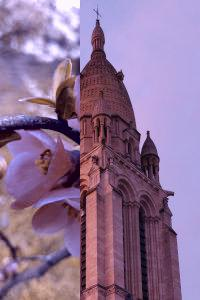
\includegraphics[align=c,width=.2\textwidth]{img/transnetv2/noslide.jpg}
    &
    &
    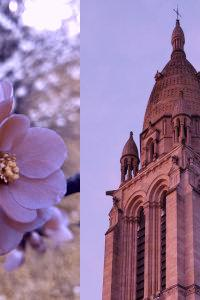
\includegraphics[align=c,width=.2\textwidth]{img/transnetv2/slide_both.jpg}
    &
    &
    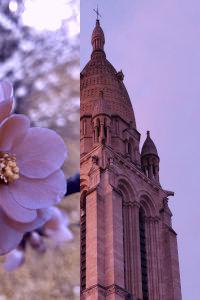
\includegraphics[align=c,width=.2\textwidth]{img/transnetv2/slide_one.jpg}
    \end{tabular}
    \caption[Examples of additional transition types]{Examples of additional transition types. Standard wipe (left), flower scene sliding in while church scene sliding out (middle) and flower scene sliding in while church scene stationary (right).}
    \label{fig:types_of_wipe}
\end{figure}
\subsubsection{Transition Types}
Similarly to the original TransNet, we generate hard cuts and dissolves. We generate 50\% of hard cuts and 50\% of dissolves, the length of each dissolve is randomly uniformly selected from the set of even lengths $\{2,4,\dots, 28, 30\}$. We generate only even lengths of dissolve transitions so that the ground truth position of the transition is exactly defined (for each frame we predict whether there is a transition from the current frame to the next frame, i.e. in case of odd lengths the transition can be either to the left or to the right of the middle frame).

As the ClipShots test set contains also wipes, we experiment with adding wipes into possible transition types. In 5\% of dissolves, we generate wipe instead of the dissolve. We consider both horizontal and vertical wipes. We also consider sliding in the entering scene, sliding out the exiting scene, or both. See Figure \ref{fig:types_of_wipe} for illustrations of different types of wipes. However, we observe no improvement in performance with wipes in the train set; therefore, we refrain from generating them.

\subsubsection{Color Transfer}
To force the network to learn more advanced local features instead of simple global features, we introduce shot color augmentation technique we call color transfer. Given two shots we transfer color from one shot $s_1$ to the other shot $s_2$ by first transforming both shots to CIE Lab color space, then we compute the new shot $s_2'$ by the following equation:
\begin{equation*}
    s_2' = \frac{\sigma_1}{\sigma_2} (s_2 - \hat{s}_2) + \hat{s}_1
\end{equation*}
where $\hat{s}_i$ is mean and $\sigma_i$ standard deviation of pixel values for respective shots. The equation is applied pixel-wise on each of the three Lab channels independently. Finally, we transform the new shot back to RGB color space. An example of the color transfer can be seen in Figure \ref{fig:color_transfer}. During training, the color transfer is applied randomly to 10\% of generated input sequences.


\begin{figure}[h]
    \centering
    \newcolumntype{C}[1]{>{\centering\arraybackslash}p{#1}}
    \begin{tabular}{cC{0.7cm}cC{0.7cm}c}
    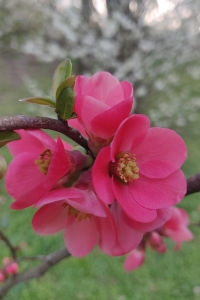
\includegraphics[align=c,width=.2\textwidth]{img/transnetv2/IMG_20190404_180509_edited.jpg}
    &
    $+$
    &
    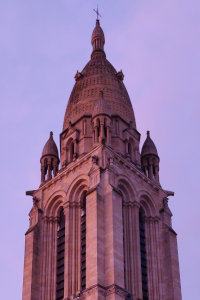
\includegraphics[align=c,width=.2\textwidth]{img/transnetv2/IMG_20200307_191029_edited.jpg}
    &
    $\rightarrow$
    &
    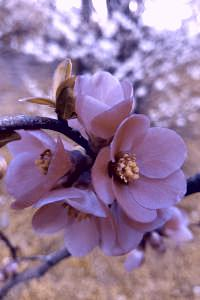
\includegraphics[align=c,width=.2\textwidth]{img/transnetv2/IMG_20190404_180509_transfered.jpg}
    \end{tabular}
    \caption[Color transfer augmentation technique between two shots]{Example of color transfer augmentation technique between two shots.}
    \label{fig:color_transfer}
\end{figure}

\subsubsection{Suppressing False Positives}
We consider adding two types of special augmentation to reduce false positives caused by handshake and rapid change of illumination e.g. by a passing object in front of a light source. Handshake is applied to five percent of train sequences by randomly removing the top (or bottom) $k\in\{1, \dots, 5\}$ pixels from the first $m$ frames and removing bottom (or top respectively) $k$ pixels from the subsequent $N-m$ frames. Finally, the frames are bilinearly resized to their original shape. Illumination change is applied to five percent of train sequences by performing the standard shot augmentation to only part of the sequence.

As the RAI dataset contains multiple sequences where color is changed between two subsequent frames, the illumination augmentation slightly improves the results. However, the opposite is seen on ClipShots and BBC datasets, where the addition of this type of augmentation creates more false negatives than it creates true negatives since these phenomena are not prevalent in these test sets.
Therefore in the final model training, we use neither artificial illumination changes nor handshake augmentation. Also, further manual inspection reveals the network can learn to suppress flashes purely from unaugmented data (Figure \ref{fig:transnetv2_predicted_transitions}A).




\subsection{Architecture Improvements}
Our TransNet V2 is based on the original TransNet network with three SDDCNN blocks, each with two DDCNN cells. However, we make a wide range of changes that substantially improve the network's performance. A schema of the TransNet V2 network is shown in Figure \ref{fig:nn_architecture_v2}, and all the changes are described in detail in the following paragraphs.

\begin{figure}
    \centering
    \begin{tikzpicture}[
    font=\sffamily\scriptsize,
    box/.style={
    	draw,
    	minimum width=0.7cm,
    	minimum height=0.4cm,
    	rounded corners=2, inner sep=2pt, align=center, anchor=north,
    	text width=1.7cm
    }, pil/.style={
    	-{Stealth[scale=.5]},
    	rounded corners=2pt,
    	line width=1pt
    }, pil2/.style={
    	rounded corners=2pt,
    	line width=1pt
    }]
    \definecolor{my-green}{RGB}{208, 240, 192}
    \definecolor{my-yellow}{RGB}{247, 231, 206}
    \definecolor{my-blue}{RGB}{195, 236, 255}
    \definecolor{my-red}{RGB}{247, 183, 183}
    
    \node[box, draw=none, text width=1cm] (input) at (0,3.3) {Input};
    \node[box, fill=my-red] (colorhist) at (2.5,-6.6) {RGB hist.\\similarities};
    \draw[pil2] (input) |- (1.5, 2.75);
    \draw[pil] (1.5, 2.75) -| (colorhist);
    
    
    \node[box, fill=my-green, text width=3cm] (layer1a) at (0,2.5) {DDCNN V2 cell\\[-2pt]{\tiny 64 filters}};
    \node[box, fill=my-green, text width=3cm] (layer1b) at (1.7,1.6) {DDCNN V2 cell\\[-2pt]{\tiny 64 filters}};
    \node[draw, circle, inner sep=1pt, align=center, anchor=north] (add1) at (0,0.9) {\textbf{+}};
    \node[box, anchor=north, fill=my-yellow] (avg-pool1) at (0,0.2) {Avg pooling\\1$\times$2$\times$2};
    
    \path[pil] (input) edge node[anchor=east] {\tiny\textit{N$\times$48$\times$27$\times$3}} (layer1a);
    \draw[pil2] (layer1a) |- (1, 1.8);
    \draw[pil] (1, 1.8) -| (layer1b);
    \draw[pil] (layer1a) -- (add1);
    \draw[pil] (layer1b) |- (add1);
    \path[pil] (add1) edge node[anchor=west] {\tiny\textit{N$\times$48$\times$27$\times$64}} (avg-pool1);
    

    \node[box, fill=my-green, text width=3cm] (layer2a) at (0,-.9) {DDCNN V2 cell\\[-2pt]{\tiny 128 filters}};
    \node[box, fill=my-green, text width=3cm] (layer2b) at (1.7,-1.8) {DDCNN V2 cell\\[-2pt]{\tiny 128 filters}};
    \node[draw, circle, inner sep=1pt, align=center, anchor=north] (add2) at (0,-2.5) {\textbf{+}};
    \node[box, anchor=north, fill=my-yellow] (avg-pool2) at (0,-3.2) {Avg pooling\\1$\times$2$\times$2};
    
    \path[pil] (avg-pool1) edge node[anchor=west] {\tiny\textit{N$\times$24$\times$13$\times$64}} (layer2a);
    \draw[pil2] (layer2a) |- (1, -1.6);
    \draw[pil] (1, -1.6) -| (layer2b);
    \draw[pil] (layer2a) -- (add2);
    \draw[pil] (layer2b) |- (add2);
    \path[pil] (add2) edge node[anchor=west] {\tiny\textit{N$\times$24$\times$13$\times$128}} (avg-pool2);

    
    \node[box, fill=my-green, text width=3cm] (layer3a) at (0,-4.3) {DDCNN V2 cell\\[-2pt]{\tiny 256 filters}};
    \node[box, fill=my-green, text width=3cm] (layer3b) at (1.7,-5.2) {DDCNN V2 cell\\[-2pt]{\tiny 256 filters}};
    \node[draw, circle, inner sep=1pt, align=center, anchor=north] (add3) at (0,-5.9) {\textbf{+}};
    \node[box, anchor=north, fill=my-yellow] (avg-pool3) at (0,-6.6) {Avg pooling\\1$\times$2$\times$2};
    
    \path[pil] (avg-pool2) edge node[anchor=west] {\tiny\textit{N$\times$12$\times$6$\times$128}} (layer3a);
    \draw[pil2] (layer3a) |- (1, -5);
    \draw[pil] (1, -5) -| (layer3b);
    \draw[pil] (layer3a) -- (add3);
    \draw[pil] (layer3b) |- (add3);
    \path[pil] (add3) edge node[anchor=west] {\tiny\textit{N$\times$12$\times$6$\times$256}} (avg-pool3);
    
    
    \node[box, text width=1.2cm] (flatten) at (0,-7.7) {Flatten};
    \path[pil] (avg-pool3) edge node[anchor=west] {\tiny\textit{N$\times$6$\times$3$\times$256}} (flatten);
    
    \node[box, text width=1.2cm] (concat) at (0,-8.5) {Concat};
    \path[pil] (flatten) edge node[anchor=west] {\tiny\textit{N$\times$4608}} (concat);
    
    \path[pil2] (colorhist) edge node[anchor=east] {\tiny\textit{N$\times$128}} (2.5, -8.5);
    \draw[pil] (2.5, -8.5) |- (concat);

    \node[box, anchor=north, fill=my-red] (framesim) at (-2.5,-6.6) {Learnable\\similarities};
    
    \draw[pil2] (avg-pool1) |- (-1, -0.65);
    \draw[pil] (-1, -0.65) -| (-2.7,-6.6);
    \draw[pil2] (avg-pool2) |- (-1, -4.05);
    \draw[pil] (-1, -4.05) -| (-2.5,-6.6);
    \draw[pil2] (avg-pool3) |- (-1, -7.45);
    \draw[pil2] (-1, -7.45) -| (-1.25, -7);
    \draw[pil2] (-1.25, -7) |- (-1.5, -6.1);
    \draw[pil] (-1.5, -6.1) -| (-2.3, -6.6);
    
    \path[pil2] (framesim) edge node[anchor=west] {\tiny\textit{N$\times$128}} (-2.5, -8.5);
    \draw[pil] (-2.5, -8.5) |- (concat);
    
    \node[box, fill=my-blue, text width=2.2cm] (dense1) at (0,-9.3) {Dense + ReLU};
    \node[box] (dropout) at (0,-10.1) {Dropout\\[-2pt]{\tiny rate 0.5}};
    \node[box, fill=my-blue] (dense2) at (-1.4,-11) {Dense};
    \node[box] (sigmoid) at (-1.4,-11.8) {Sigmoid};
    \node[box, fill=my-blue] (dense2-multihead) at (1.4,-11) {Dense};
    \node[box] (sigmoid-multihead) at (1.4,-11.8) {Sigmoid};
    
    \path[pil] (concat) edge node[anchor=west] {\tiny\textit{N$\times$4864}} (dense1);
    \path[pil] (dense1) edge node[anchor=west] {\tiny\textit{N$\times$1024}} (dropout);
    \draw[pil2] (dropout) |- (-1,-10.8);
    \draw[pil] (-1,-10.8) -| (dense2);
    \draw[pil2] (dropout) |- (1,-10.8);
    \draw[pil] (1,-10.8) -| (dense2-multihead);
    \path[pil] (dense2) edge node[anchor=west] {\tiny\textit{N$\times$1}} (sigmoid);
    \path[pil] (dense2-multihead) edge node[anchor=west] {\tiny\textit{N$\times$1}} (sigmoid-multihead);
    
    \draw[decorate,decoration={brace}] (-2.4,-12.2) -- (-2.4,-11) node[midway, anchor=center,sloped, above=0.1, font=\sffamily\tiny, align=center] {Single transition\\frame prediction};
    \draw[decorate,decoration={brace}] (2.4,-11) -- (2.4,-12.2) node[midway, anchor=center,sloped, above=0.1, font=\sffamily\tiny, align=center] {All transition\\frames prediction};

    %
    %
    
    \end{tikzpicture}
    \caption[TransNet V2 shot boundary detection network architecture]{TransNet V2 shot boundary detection network architecture. Note that $N$ represents the length of a video sequence, not batch size.}
    \label{fig:nn_architecture_v2}
\end{figure}


\subsubsection{Convolution Kernel Factorization}
The TransNet benefits from using four decoupled convolutions instead of a single one since the decoupling reduces the number of parameters and the network is less prone to over-fitting, and also speeds up the computation. We further investigate how to factorize the convolution kernel to reduce over-fitting while preserving the benefits of a large field of view. In the image domain, depthwise separable convolutions have been introduced. The depthwise spatial convolution acts on each input channel separately and is followed by a pointwise (the standard $1\times 1$) convolution, which combines the resulting output channels. This way, the network is limited to learn only factorizable kernels; however, Chollet \cite{Chollet_2017_CVPR} shows it improves classification performance of InceptionV3 network \cite{Szegedy_2016_InceptionV3} on ImageNet \cite{imagenet}.

In video domain, Xie et al. \cite{Xie_2018_ECCV} disentangles 3D $k \times k \times k$ convolutions into 2D $k\times k$ spatial convolution and 1D temporal convolution with kernel size $k$ to improve I3D's \cite{Carreira_2017_CVPR} performance on multiple datasets. Practically the separable 3D convolution can be implemented by two standard 3D convolutions with kernel shapes $1 \times k \times k$ for the spatial and $k \times 1 \times 1$ for the temporal convolution. This factorization of the convolutional kernel forces the network to learn to extract image features in the first step and to compare them temporarily in the second step. It also potentially reduces number of trainable parameters -- $N_{in}\times k^2\times F$ for the spatial kernel and $F\times k\times N_{out}$ for the temporal kernel compared to standard $N_{in}\times k^3\times N_{out}$. If the number of input filters $N_{in}$ is the same as output filters $N_{out}$, then if the number of filters $F$ in between the spatial and temporal convolution is smaller than $N_{out}\cdot k^3 / (k^2 + k)$, the number of trainable parameters of the separable 3D convolution is lower than the number of parameters of the standard convolution. For kernel size $k=3$ we may select any $F < 2.25 N_{out}$ while still lowering the parameter count.

In our case, we observe that setting $F=N_{out}$ is too extreme parameter reduction, hampering the performance of the model. However, setting $F=2 N_{out}$ improves the performance substantially. Figure \ref{fig:ddcnnv2} shows the new version of the DDCNN block with factorized convolutions.

\begin{figure}
    \centering
    \begin{tikzpicture}[
    font=\sffamily\scriptsize,
    box/.style={
    	draw,
    	minimum width=0.7cm,
    	minimum height=0.4cm,
    	rounded corners=2, inner sep=2pt, align=center, anchor=north,
    	text width=1.7cm
    }, pil/.style={
    	-{Stealth[scale=.5]},
    	rounded corners=2pt,
    	line width=1pt
    }]
    \definecolor{my-green}{RGB}{208, 240, 192}
    \definecolor{my-yellow}{RGB}{247, 231, 206}
    \definecolor{my-blue}{RGB}{195, 236, 255}

    
    \node[box, draw=none, text width=1cm] (input) at (0,3) {Input};
    
    %%% DDCNN cell
    \node[box, fill=my-green] (layer1-1) at (-3,2) {Conv 1$\times$3$\times$3};
    \node[box, fill=my-green] (layer1-2) at (-1,2) {Conv 1$\times$3$\times$3};
    \node[box, fill=my-green] (layer1-3) at (1,2) {Conv 1$\times$3$\times$3};
    \node[box, fill=my-green] (layer1-4) at (3,2) {Conv 1$\times$3$\times$3};
    
    \node[box, fill=my-green] (layer2-1) at (-3,1.2) {Conv 3$\times$1$\times$1\\[-2pt]{\tiny dilation 1}};
    \node[box, fill=my-green] (layer2-2) at (-1,1.2) {Conv 3$\times$1$\times$1\\[-2pt]{\tiny dilation 2}};
    \node[box, fill=my-green] (layer2-3) at (1,1.2) {Conv 3$\times$1$\times$1\\[-2pt]{\tiny dilation 4}};
    \node[box, fill=my-green] (layer2-4) at (3,1.2) {Conv 3$\times$1$\times$1\\[-2pt]{\tiny dilation 8}};
    
    \node[box, text width=1.2cm] (layer-out) at (0,0.4) {Concat};
    
    \node[box, anchor=north, fill=my-yellow, text width=3cm] (bn) at (0,-0.4) {Batch Normalization};
    
    \node[box, text width=1.2cm] (relu) at (0,-1.) {ReLU};

    %%% EDGES
    \draw[rounded corners=2pt, line width=1pt] (input) |- (-0.3,2.3);
    \draw[rounded corners=2pt, line width=1pt] (input) |- (0.3,2.3);
    
    \draw[pil] (-0.3,2.3) -| (layer1-1);
    \draw[pil] (-0.3,2.3) -| (layer1-2);
    \draw[pil] (0.3,2.3) -| (layer1-3);
    \draw[pil] (0.3,2.3) -| (layer1-4);

    \draw[pil] (layer1-1) edge node[anchor=east] {\tiny 2F filters} (layer2-1);
    \draw[pil] (layer1-2) edge node[anchor=east] {\tiny 2F filters} (layer2-2);
    \draw[pil] (layer1-3) edge node[anchor=west] {\tiny 2F filters} (layer2-3);
    \draw[pil] (layer1-4) edge node[anchor=west] {\tiny 2F filters} (layer2-4);
    
    \draw[line width=1pt] (layer2-1) edge node[anchor=east,near end] {\tiny F filters} (-3, 0.32);
    \draw[line width=1pt] (layer2-2) edge node[anchor=east,near end] {\tiny F filters} (-1, 0.32);
    \draw[line width=1pt] (layer2-3) edge node[anchor=west,near end] {\tiny F filters} (1, 0.32);
    \draw[line width=1pt] (layer2-4) edge node[anchor=west,near end] {\tiny F filters} (3, 0.32);
    
    \draw[pil] (-3, 0.32) |- (layer-out);
    \draw[pil] (-1, 0.32) |- (layer-out);
    \draw[pil] (1, 0.32) |- (layer-out);
    \draw[pil] (3, 0.32) |- (layer-out);
    
    \draw[pil] (layer-out) edge node[anchor=west] {\tiny 4F filters} (bn);
    \draw[pil] (bn) -- (relu);
    

    \end{tikzpicture}
    \caption[DDCNN V2 cell with 4F filters]{DDCNN V2 cell with 4F filters.}
    \label{fig:ddcnnv2}
\end{figure}

\subsubsection{Frame Similarities as Features}
As already discussed in the related work section, many methods extract individual frame features and use them to compute similarity scores between consequent frames. The scores are then used as an input to a machine learning model such as SVM that predicts the likelihood of transition purely from the similarity scores. Similarly, we improve the performance of TransNet's final fully-connected classifier by enriching the convolutional features by frame similarities. We consider frame similarities computed both from handcrafted and learnable features. A simple RGB color histogram with $8^3=512$ bins is used for the handcrafted features. For the learnable features, we take outputs of all SDDCNN blocks. Those outputs of shape $N\times H_l \times W_l \times C_l$ are spatially averaged into vectors of shape $N \times C_l$ and vectors from different levels $l$ are concatenated thus every one of the $N$ frames is represented by vector $v_i$ of length $\sum_{l=0}^L C_l$. A single linear layer without activation function is applied to reduce the dimension of the vector $v_i$ to 128.

For each frame, we compute cosine similarities of its handcrafted or learned features with fifty frames preceding the frame and fifty frames following the frame. The similarities are transformed by a single fully connected layer with the ReLU activation function into 128-dimensional space and are concatenated with the convolutional features. If not all of the fifty preceding or following frames are available due to the limited length $N$ of the input sequence zeros are used instead. Figure \ref{fig:frame_sim} depicts such computation for the learned features.

\begin{figure}
    \centering
    \begin{tikzpicture}[
    font=\sffamily\scriptsize,
    box/.style={
    	draw,
    	minimum width=0.7cm,
    	minimum height=0.4cm,
    	rounded corners=2, inner sep=2pt, align=center, anchor=north,
    	text width=1.7cm
    }, pil/.style={
    	-{Stealth[scale=.5]},
    	rounded corners=2pt,
    	line width=1pt
    }, pil2/.style={
    	rounded corners=2pt,
    	line width=1pt
    }, table/.style={
        matrix of nodes,
        row sep=-\pgflinewidth,
        column sep=-\pgflinewidth,
        nodes={
            rectangle,
            draw=black,
            align=center,
            inner sep=0pt,
            minimum height=0.35cm,
            text width=0.35cm,
        },
        font=\sffamily\tiny,
        nodes in empty cells,
    }]
    \definecolor{my-gray}{RGB}{251, 251, 251}
    \definecolor{my-yellow}{RGB}{247, 231, 206}
    \definecolor{my-blue}{RGB}{195, 236, 255}
    \definecolor{my-red}{RGB}{247, 183, 183}
    \definecolor{my-green}{RGB}{208, 240, 192}

    
    \node[box, draw=none, text width=1cm] (input) at (0,3) {Inputs};
    
    %%% DDCNN cell
    \node[box, fill=my-yellow, text width=1.2cm] (avg1) at (-1.5,2) {Spatial\\average};
    \node[box, fill=my-yellow, text width=1.2cm] (avg2) at (0,2) {Spatial\\average};
    \node[box, fill=my-yellow, text width=1.2cm] (avg3) at (1.5,2) {Spatial\\average};
    
    \path[pil] (-1.5, 2.4) edge node[anchor=east] {\tiny\textit{N$\times$24$\times$13$\times$64}} (avg1);
    \path[pil] (-.4, 2.4) edge node[anchor=west] {\tiny\textit{N$\times$12$\times$6$\times$128}} (-.4,2);
    \path[pil] (1.5, 2.4) edge node[anchor=west] {\tiny\textit{N$\times$6$\times$3$\times$256}} (avg3);
    
    \node[box, text width=1.2cm] (concat) at (0,0.9) {Concat};
    \node[box, fill=my-blue] (dense1) at (0,0.1) {Dense};
    
    \node[box, draw=lightgray, text width=3.4cm, text height=1.9cm, fill=my-gray] at (0.35,-0.65) {};
    \node[rotate=90, text=gray] at (-1.2, -1.7) {Cosine Sim};
    \node[box, fill=my-yellow] (normalize) at (0,-0.7) {Normalize};
    \node[box] (transpose) at (1.1,-1.4) {Transpose};
    \node[box] (matmul) at (0,-1.9) {Matrix\\Multiplication};
    
    \node[box, text width=2.2cm, fill=my-red] (gather) at (0,-3) {Pad + Gather};
    \node[box, fill=my-blue, text width=2.2cm] (dense2) at (0,-3.8) {Dense + ReLU};
    
    \path[pil2] (avg1) edge node[anchor=east] {\tiny\textit{N$\times$64}} (-1.5, 0.9);
    \path[pil] (avg2) edge node[anchor=west] {\tiny\textit{N$\times$128}} (concat);
    \path[pil2] (avg3) edge node[anchor=west] {\tiny\textit{N$\times$256}} (1.5, 0.9);
    \draw[pil] (-1.5, 0.95) |- (concat);
    \draw[pil] (1.5, 0.95) |- (concat);
    
    \path[pil] (concat) edge node[anchor=west] {\tiny\textit{N$\times$448}} (dense1);
    \path[pil] (dense1) edge node[anchor=west] {\tiny\textit{N$\times$128}} (normalize);
    \path[pil] (matmul) edge node[anchor=west] {\tiny\textit{N$\times$N}} (gather);
    \path[pil] (gather) edge node[anchor=west] {\tiny\textit{N$\times$101}} (dense2);
    \path[pil] (dense2) edge node[anchor=west] {\tiny\textit{N$\times$128}} (0,-4.6);
    
    \draw[pil2] (normalize) |- (0.5, -1.2);
    \draw[pil] (0.5, -1.2) -| (transpose);
    
    \draw[pil] (transpose) |- (matmul);
    \draw[pil] (normalize) -- (matmul);
    

    \matrix (table1) [table] at (6,-0.1){
    |[fill=my-green!100]|1  & |[fill=my-green!70]|.8 & |[fill=my-green!35]|.6 & .6 & .4 \\
    |[fill=my-green!70]|.8 &  |[fill=my-green!100]|1 & |[fill=my-green!70]|.7 & |[fill=my-green!35]|.7 & .5 \\
    |[fill=my-green!35]|.6 & |[fill=my-green!70]|.7 &  |[fill=my-green!100]|1 & |[fill=my-green!70]|.9 & |[fill=my-green!35]|.6 \\
    .6 & |[fill=my-green!35]|.7 & |[fill=my-green!70]|.9 &  |[fill=my-green!100]|1 & |[fill=my-green!70]|.7 \\
    .4 & .5 & |[fill=my-green!35]|.6 & |[fill=my-green!70]|.7 &  |[fill=my-green!100]|1 \\
    };
    
    \node[box, text width=2.2cm, fill=my-red, anchor=center] (gather2) at (6,-1.5) {Pad + Gather};
    
    \matrix (table2) [table] at (6,-2.9){
    0  &  0 & |[fill=my-green!100]|1  & |[fill=my-green!70]|.8 & |[fill=my-green!35]|.6 \\
    0  & |[fill=my-green!70]|.8 & |[fill=my-green!100]|1  & |[fill=my-green!70]|.7 & |[fill=my-green!35]|.7 \\
    |[fill=my-green!35]|.6 & |[fill=my-green!70]|.7 & |[fill=my-green!100]|1  & |[fill=my-green!70]|.9 & |[fill=my-green!35]|.6 \\
    |[fill=my-green!35]|.7 & |[fill=my-green!70]|.9 & |[fill=my-green!100]|1  & |[fill=my-green!70]|.7 & 0  \\
    |[fill=my-green!35]|.6 & |[fill=my-green!70]|.7 & |[fill=my-green!100]|1  & 0  & 0  \\
    };

    \path[pil] (6, -0.98) edge (gather2);
    \path[pil] (gather2) edge (6, -2.02);

    \end{tikzpicture}
    \caption[Learnable frame similarities computation with visualization of Pad + Gather operation]{Learnable frame similarities computation with visualization of Pad + Gather operation (right).}
    \label{fig:frame_sim}
\end{figure}

\subsubsection{Shortcuts}
Some transitions are easy to detect by simple differencing in a minimal number of layers, others need the full depth of the network to be detected. We add a residual connection in each Stacked DDCNN block from the output of the first DDCNN cell in the block to the input of the spatial pooling operation.% Intuitively we think of the residual connections as short paths for easy transitions.

\subsubsection{Batch Normalization}
Neural network training is dependent on the initialization of the network's parameters. If parameters are not initialized carefully, activations inside the network can rise to extreme values, which in turn can result in getting stuck in poor local minima. We employ batch normalization technique \cite{BatchNormalization} that normalizes outputs of each layer by mean and variance computed from the input batch. It allows us to worry less about the learning rate and be less careful about parameter initialization. More importantly, it also acts as a regularizer, so the network is less prone to over-fitting.

\subsubsection{Multiple Classification Heads}
The original TransNet predicts every transition as a single frame transition, no matter the length. This representation has its benefit that (almost) every frame belongs to a scene -- no frames are `inside' a transition. Further, if two transitions are very close to each other, there is no ambiguity if it is a single long transition or two separate transitions. However, this representation does not provide information on transition length. Therefore we add a second prediction head that predicts all in-transition frames instead of only the middle one. 
In some of our preliminary experiments adding the second head slightly improves performance. We hypothesize the network can learn more easily what constitutes as a transition and how long the transition is. Note that even though the information on the length of a transition is readily available, we do not use it in any way in the evaluation phase. However, we believe utilizing this information could, for example, eliminate many double detections when a single long transition is detected multiple times.


\subsection{Other Changes}

\subsubsection{Optimizer}
In recent years there have been countless efforts to improve the standard stochastic gradient descent optimization method. RMSProp \cite{tieleman2012lecture} and Adam \cite{Adam14} have become some of the most widely adopted optimizers with both utilizing estimates of gradients' second moments. However, many state-of-the-art works in the image domain \cite{autoaugment, EfficientNet} refrain from using them and instead use rather primitive stochastic gradient descent with momentum while achieving better results. In our task, we observe that Adam optimizer is more effective in minimizing the loss than SGD with momentum; however, we see performance improvements on validation and test sets when using SGD with momentum compared to Adam.

\subsubsection{Regularization}
Artificially generated training data distribution is inherently different from the real data distribution. To reduce generalization error, we restrict the model's parameter space by also minimizing the square of $L_2$ norm of the parameters. Such action increases error on artificially generated validation data; however, it greatly reduces error on real data. Given the work of Loshchilov et al. \cite{FixingWeightDecay}, we also investigate whether decoupling the $L_2$ regularization from optimizer step computation -- a technique known as weight decay -- affects model's performance. While $L_2$ regularization and weight decay are (after hyper-parameter re-scaling) equivalent in the case of vanilla SGD, in more advanced optimizers, gradient moments estimations are affected by the square of $L_2$ norm of parameters in the loss. Loshchilov et al. argue this phenomenon is responsible for the inferior performance of Adam. However, in our case, when using SGD with momentum, we do not see any significant difference between $L_2$ regularization and weight decay.

Another form of regularization we employ is Dropout \cite{dropout}. It addresses the over-fitting problem by randomly dropping units from the neural network during training. In TransNet V2, we drop activations of the first fully-connected layer with a probability $0.5$.

\subsubsection{Class Imbalance}
The main classification head of the network is trained with only one frame labeled as transition and the other frames as no transition. In the case of long dissolve transitions, missing the middle transition frame even by a single position results in a large penalty; therefore, the network is inclined not to predict these transitions with high confidence at all. The original TransNet solves the problem by adjusting the decision threshold to $0.1$. We look at the problem more generally and weight the positive class by $\gamma$. Based on the exact task and dataset at hand, we may increase or decrease $\gamma$ to increase recall or precision respectively. For example, in retrieval, 100\% recall is crucial, whereas high precision may be preferred elsewhere. %in commercial shot detection applications as false positives are right in front of user's eyes wheres undetected transition will likely remain undiscovered by the user therefore not damaging user's satisfaction with the product {\color{red} TODO - to bych asi netvrdil}.
In our experiments, $\gamma = 5$ is used.

\subsubsection{Loss Function}
To train both classification heads we use the standard cross entropy loss (Equation~\ref{eq:transnetv2_cross_entropy}) with sequence predictions $\hat{y}$, sequence ground truth $y$ and possibly a weight $w$ of the positive \textit{is-a-transition} class. Since we predict likelihood of a transition for every frame in an input frame sequence $\bm{x}$ of length $N$, the length of $\hat{y}$ and $y$ vectors is also $N$.
\begin{equation}
  \mathcal{L}(\hat{y}, y, w)=-\sum_{i=1}^{N} \big[ w y_i\log \hat{y}_i + (1-y_i)\log(1-\hat{y}_i) \big]
  \label{eq:transnetv2_cross_entropy}
\end{equation}
The joint objective is shown in Equation \ref{eq:transnetv2_loss}. The first term is the loss of the classification head $f^s$ predicting single transition frame for arbitrarily long transition, the second term is the loss of the classification head $f^a$ predicting all transition frames and is weighted by $\lambda_a=0.1$. These loss terms are averaged over the batch. Last term of the objective is $L_2$ regularization of model's parameters $\theta$ weighted by $\lambda_p=0.0001$.
\begin{equation}
    \min \frac{1}{|\mathcal{B}|} \sum_{\left(\bm{x},y^s,y^m\right)\in\mathcal{B}} \Big[ \mathcal{L}\big(f^s(\bm{x};\theta), y^s, \gamma\big) + \lambda_a \mathcal{L}\big(f^a(\bm{x};\theta), y^a, 1\big) \Big] + \frac{\lambda_p}{2} \sum_{\vartheta\in\theta}\|\vartheta\|^2_2 
    \label{eq:transnetv2_loss}
\end{equation}
In Figure \ref{fig:input_sample} we show a sample frame sequence $\bm{x}$ with both immediate and gradual transition and its two types of ground truth vectors $y^s$ and $y^a$ for the two classification heads. Note that artificially generated train frame sequences contain only a single transition per sequence; however, when training with real data, it is possible to have multiple transitions in a single frame sequence if the transitions are close to each other.

\begin{figure}
    \centering
    \begin{tikzpicture}[
    box/.style={
    	draw,
    	minimum width=1cm,
    	minimum height=0.6cm,
    	align=center,
    	anchor=center
    },
    element1/.style={
        draw,
        minimum width=0.4cm,
    	minimum height=0.4cm,
    	align=center,
    	anchor=center,
    	circle
    },
    element2/.style={
        draw,
    	inner sep=2.8pt,
    	align=center,
    	anchor=center,
    	diamond
    }]
    \definecolor{g1}{RGB}{220, 220, 220}
    \definecolor{g2}{RGB}{180, 180, 180}
    \definecolor{g3}{RGB}{140, 140, 140}
    \definecolor{g4}{RGB}{70, 70, 70}

    \node[align=center,anchor=center] at (-2.,0) {$\bm{x}$};
    \node[align=center,anchor=center] at (-2.,-0.7) {$y^s$};
    \node[align=center,anchor=center] at (-2.,-1.3) {$y^a$};
    \node[align=center,anchor=center] at (-1.2,0) {$=$};
    \node[align=center,anchor=center] at (-1.2,-0.7) {$=$};
    \node[align=center,anchor=center] at (-1.2,-1.3) {$=$};
   
    \node[align=center,anchor=center] at (0,-0.7) {$0$};
    \node[align=center,anchor=center] at (1.2,-0.7) {$0$};
    \node[align=center,anchor=center] at (2.4,-0.7) {$1$};
    \node[align=center,anchor=center] at (3.6,-0.7) {$0$};
    \node[align=center,anchor=center] at (4.8,-0.7) {$0$};
    \node[align=center,anchor=center] at (6,-0.7) {$0$};
    \node[align=center,anchor=center] at (7.2,-0.7) {$1$};
    \node[align=center,anchor=center] at (8.4,-0.7) {$0$};
    
    \node[align=center,anchor=center] at (0,-1.3) {$0$};
    \node[align=center,anchor=center] at (1.2,-1.3) {$1$};
    \node[align=center,anchor=center] at (2.4,-1.3) {$1$};
    \node[align=center,anchor=center] at (3.6,-1.3) {$1$};
    \node[align=center,anchor=center] at (4.8,-1.3) {$1$};
    \node[align=center,anchor=center] at (6,-1.3) {$0$};
    \node[align=center,anchor=center] at (7.2,-1.3) {$1$};
    \node[align=center,anchor=center] at (8.4,-1.3) {$0$};
    
    \node[box] (img1) at (0,0) {};
    \node[box] (img2) at (1.2,0) {};
    \node[box] (img3) at (2.4,0) {};
    \node[box] (img4) at (3.6,0) {};
    \node[box] (img5) at (4.8,0) {};
    \node[box] (img6) at (6,0) {};
    \node[box] (img7) at (7.2,0) {};
    \node[box] (img8) at (8.4,0) {};
    
    \node[element1] at (img1) {};
    \node[element1, g4] at (img2) {};
    \node[element1, g3] at (img3) {};
    \node[element1, g2] at (img4) {};
    \node[element1, g1] at (img5) {};
    \node[element1] at (img8) {};


    \node[element2, g1] at (img2) {};
    \node[element2, g2] at (img3) {};
    \node[element2, g3] at (img4) {};
    \node[element2, g4] at (img5) {};
    \node[element2] at (img6) {};
    \node[element2] at (img7) {};

    \end{tikzpicture}
    \caption[Frame sequence with its ground truth]{Frame sequence with its two types of ground truth.}
    \label{fig:input_sample}
\end{figure}




\clearpage
\section{Experiments}\label{sec:transnetv2_evaluation}
In this section, we describe in detail the training process of the TransNet V2 model. Further, we compare our model to related works, also detailing our reevaluation process for it. Lastly, an ablation study is made to justify our decisions in making TransNet V2.

\subsection{Training Details}
We initialize weights of all convolution operations by He normal initializer~\cite{He_2015_ICCV}. Fully connected layers are initialized by TensorFlow's default Glorot initiali\-zer~\cite{Xavier_Glorot_init}. Biases are initialized by zeros.
We optimize the loss function (Equation \ref{eq:transnetv2_loss}) by stochastic gradient descent with momentum set to $0.9$ and fixed learning rate~$0.01$.

The standard TransNet V2 model is trained only by artificially generated sequences from IACC.3 and ClipShots datasets as described in Section \ref{sec:transnetv2DatasetsAugm}. Fifty percent of transitions we generate are hard cuts and fifty percent are dissolves of max length 30 frames. Besides, we consider training TransNet V2 by 15\% of real transitions from the ClipsShots dataset, 35\% of automatically generated hard cuts, and 50\% of automatically generated dissolves. Input to the network is frame sequences of length $N=100$ with each frame of size 48$\times$27.

We train the network for 30 epochs, each with 750 batches of size 16. In case the network is trained also in part by real manually annotated transitions from the ClipShots dataset, we add 20 additional epochs, i.e. the network is trained in total by 600,000 transitions. Training by artificial data only longer than 30 epochs is unnecessary since the network then overfits. The best performing model on our ClipShots validation set is selected. Together with validation, the training takes approximately 17 hours on a single Tesla V100 16GB GPU. TensorFlow deep learning library has been used for all the experiments.

\subsection{Results}
We report results of TransNet V2 trained both with artificial data only and with 15\% of real data. Additionally, we report the results of the original TransNet retrained by our data generation pipeline (Section \ref{sec:transnetv2DatasetsAugm}). For each network we show mean F1 scores\footnote{The same evaluation metric as in Section \ref{sec:transnetV1Eval} is used. However, due to minor errors in ground truth of some test sets, we also count correctly any detection that misses ground truth by at most two frames. With correct ground truth its effect compared to the original metric is minimal.\label{fn:metric}} and their standard deviations on the test sets in Table \ref{tb:transnets_results}. The statistics are computed from three best epochs from each of three independent runs as measured on the ClipShots validation dataset. We see a clear dominance of TransNet V2, especially on the ClipShots dataset. Utilizing real transitions improves results on BBC Planet Earth dataset while it harms performance on ClipShots and especially on RAI. We further discuss this phenomenon of better results with artificially generated data compared to the real data in the next section.

\begin{table}[h]
	\centering
	\begin{tabular}{l@{\hspace{1cm}}cccc}
		\toprule
		\textbf{Model} & ClipShots & BBC  & RAI \\
		\midrule
		TransNet                             & $71.9 \pm 3.5$ & $94.0 \pm 0.6$ & $93.1 \pm 0.6$ \\
		TransNet V2                          & $\bm{77.5} \pm 0.3$ & $95.1 \pm 0.5$ & $\bm{93.2} \pm 0.9$ \\
		TransNet V2 (15\% real transitions)  & $77.0 \pm 0.8$ & $\bm{96.5} \pm 0.5$ & $91.2 \pm 1.1$ \\
		\bottomrule
	\end{tabular}
	\caption[Comparison of the original TransNet and TransNet V2]{Comparison of the original TransNet and TransNet V2. Mean F1 scores and standard deviations in percents. Computed from 9 model instances (3 best epochs of 3 independent runs as measured on ClipShots validation set).}
	\label{tb:transnets_results}
\end{table}

We compare TransNet V2 to related work in Table \ref{tb:transnet_related_work}. For TransNet models, we report the F1 score of the best model selected out of the nine instances based on its performance on the ClipShot validation set. To best of our knowledge, the best shot boundary detectors available, as reported by their authors, are DeepSBD by Hassanien et al., DSM by Tang et al., and our original TransNet. On RAI dataset these methods report F1 score 93.4\%, 93.5\%, and 94.3\% respectively. However, Hassanien et al. report results on neither ClipShots nor BBC dataset. Tang et al. report results on ClipShots but their validation method differs from our method\footref{fn:metric} described in Section \ref{sec:transnetV1Eval} and for example incorrectly counts double detection. Therefore we reevaluate both shot boundary detection models and report only these results. We discuss reevaluation details in Section \ref{sec:transnetv2Reevaluation}.

\begin{table}[h]
	\centering
	\sisetup{detect-weight=true,detect-inline-weight=math}
	\begin{tabular}{l@{\hspace{1cm}}S[table-format=2.1]S[table-format=2.1]S[table-format=2.1]}
		\toprule
		\textbf{Model} & \multicolumn{1}{c}{ClipShots} & \multicolumn{1}{c}{BBC}  & \multicolumn{1}{c}{RAI} \\
		\midrule
		TransNet                             & 74.8 & 94.6 & 93.4 \\
		TransNet V2                          & 77.5 & 95.8 & \bftabnum 94.4 \\
		TransNet V2 (15\% real transitions)  & \bftabnum 77.9 & \bftabnum 96.2 & 93.9 \\
		\midrule
		TransNet\textsuperscript{$\dagger$}        & 73.5 & 92.9 &  94.3 \\
        Hassanien et al. \cite{Hassanien17}             & 75.9\textsuperscript{$*$} & 92.6\textsuperscript{$*$} & 93.9\textsuperscript{$*$} \\
        Tang et al. \cite{Tang2018}, ResNet baseline & 76.1\textsuperscript{$*$} & 89.3\textsuperscript{$*$} & 92.8\textsuperscript{$*$} \\
		\bottomrule
		\multicolumn{4}{l}{\footnotesize \textsuperscript{$\dagger$} The original TransNet as reported in Chapter \ref{sec:transnetv1} and in \cite{soucek2019transnet}. Reevaluated.} \\
		\multicolumn{4}{l}{\footnotesize \textsuperscript{$*$} Our reevaluation with the best threshold. See Section \ref{sec:transnetv2Reevaluation} for more details.}  \\
	\end{tabular}
	\caption[Comparison of TransNet V2 with related work]{Comparison of TransNet V2 with related work. F1 scores in percents. In the case of TransNet entries, the model with the best F1 score on the validation set is shown.}
	\label{tb:transnet_related_work}
\end{table}


TransNet V2 clearly outperforms related work on both ClipShots and BBC Planet Earth datasets, on the latter almost halving the error achieved by the previous state-of-the-art. On the RAI dataset, all methods perform comparably. Relative low performance on ClipShots can be attributed to the fact that it contains multiple seemingly unannotated videos or video parts. Further, in many cases, a frame is annotated as a transition incorrectly. We show some interesting transitions with our predictions in Figure \ref{fig:transnetv2_predicted_transitions} to illustrate our model's strengths and weaknesses, in Figure \ref{fig:transnet_v1_v2_visualization_comparison} raw predictions are shown on a long video sequence comparing the original TransNet and TransNet V2. Here we list some of the main takeaways:
\begin{itemize}
    \item Many times the ground truth incorrectly labels flash as a transition; however, the model can correctly ignore it. Nonetheless, if there is an illumination change in multiple subsequent frames, the model struggles (Figure \ref{fig:transnetv2_predicted_transitions}A).
    \item Long transitions with custom animations or fade-ins with uncommon colors are usually missed by the model (Figure \ref{fig:transnetv2_predicted_transitions}B, only selected frames from the transition shown).
    \item It can happen that the model misses a transition that is easily distinguishable for humans. However, sometimes these transitions are missing in the ground truth data (Figure \ref{fig:transnetv2_predicted_transitions}C).
    \item The model struggles with heavy motion blur (Figure \ref{fig:transnetv2_predicted_transitions}D).
    \item Many times it is subjective whether there is a transition (Figure \ref{fig:transnetv2_predicted_transitions}E).
\end{itemize}
All in all, on ClipShots dataset the best instance of TransNet V2 achieves 5.7k true positives, 1.7k false positives, and 1.5k false negatives. This is in stark contrast to BBC Planet Earth dataset, where the model achieves almost six times as many false negatives as false positives (exactly 4537 true positives, 55 false positives, and 307 false negatives). Such discrepancy can be attributed to already mentioned missing annotations and many long, difficult, and sometimes ambiguous transitions in ClipShots dataset.

Concerning the RAI dataset, all models perform comparably with a slight exception of Tang et al. However, we refrain from making any conclusions as the dataset contains mainly TV shows with visual effects that account for possibly many ambiguities in the ground truth. For example, the frame sequence in Figure \ref{fig:ambiguous_sequence_rai} is contained with slight variations in the dataset more than 20 times, and classifying it as transitions can result in almost doubling the number of false positives achieved by our method.

\begin{figure}[h]
    \centering
    \begin{tikzpicture}

    \node[inner sep=0pt] at (-5.2,0)
    {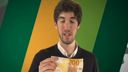
\includegraphics[width=2.4cm]{img/transnetv2/rai_scene/000.jpg}};
    \node[inner sep=0pt] at (-2.6,0)
    {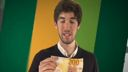
\includegraphics[width=2.4cm]{img/transnetv2/rai_scene/001.jpg}};
    \node[inner sep=0pt] at (0,0)
    {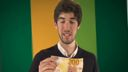
\includegraphics[width=2.4cm]{img/transnetv2/rai_scene/002.jpg}};
    \node[inner sep=0pt] at (2.6,0)
    {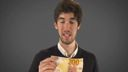
\includegraphics[width=2.4cm]{img/transnetv2/rai_scene/003.jpg}};
    \node[inner sep=0pt] at (5.2,0)
    {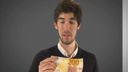
\includegraphics[width=2.4cm]{img/transnetv2/rai_scene/004.jpg}};
    
    %\draw[-{to reversed[scale=.4]}, thick] (-6.4, -0.85) -- (-2.6, -0.85);
    %\draw[{to reversed[scale=.4]}-, thick] (0, -0.85) -- (6.4, -0.85);
    %\draw[dotted] (-6.4, -1) -- (6.4, -1);
    %\node at (0, -1.1) {};
    \end{tikzpicture}
    \caption[Ambiguous frame sequence from the RAI dataset]{Ambiguous frame sequence from the RAI dataset labeled as \textit{no-transition} in the ground truth data.}
    \label{fig:ambiguous_sequence_rai}
\end{figure}


There are many more ambiguities similar to Figure \ref{fig:ambiguous_sequence_rai}; therefore we conclude it is necessary to adjust the model's threshold or even training data to compensate for particularities of a task at hand in case the reader's definition of a transition differs from our train and test data. For that reason, we show precision-recall curves and F1 scores as a function of the model's threshold for our best model TransNet V2 trained with 15\% real transitions on all test sets (Figure \ref{fig:transnetv2_prcurve}).

\begin{figure}[h]
    \centering
    \definecolor{my-red}{RGB}{255,51,76}
    \definecolor{my-green}{RGB}{63,188,157}
    \definecolor{my-blue}{RGB}{25,116,210}
    
    \begin{tikzpicture}[/pgfplots/width=\linewidth, /pgfplots/height=\linewidth]
    \begin{axis}[% Axis labels
                 ymin=.6,ymax=1,xmin=0,xmax=1,
    			 % Axis labels
    			 table/col sep=comma,
        		 xlabel={Recall / Threshold},
        		 ylabel={Precision / F1},
         		 xlabel shift={-2pt},
        		 ylabel shift={-3pt},
         		 % General appearance
		         font=\small,
		         axis equal image=true,
		         enlargelimits=false,
		         clip=true,
		         nodes near coords, % Place nodes near each coordinate
		         point meta=explicit symbolic,
		         % Grids 
        	     grid style=dotted, grid=both,
                 major grid style={white!65!black},
        		 minor grid style={white!85!black},
		 		 xtick={0,0.1,...,1.1},
        		 ytick={0,0.1,...,1.1},
         		 minor xtick={0,0.02,...,1},
		         minor ytick={0,0.02,...,1},
        		 % Legend
        		 legend style={at={(0,0)},
                 		       anchor=south west}]
        
	\addlegendimage{/pgfplots/refstyle=plot:prplot,black}\addlegendentry{P/R curve}
    \addlegendimage{/pgfplots/refstyle=plot:f1plot,black}\addlegendentry{F1/Thr curve}
    \addlegendimage{my-green}\addlegendentry{ClipShots}
    \addlegendimage{my-blue}\addlegendentry{BBC}
    \addlegendimage{my-red}\addlegendentry{RAI}

    \addplot[my-green,mark size=1.7,thick,mark repeat=5, mark phase=5,mark=*,font=\scriptsize] table[x=Recall,y=Precision, meta index=0] {data/transnetv2-prcurve-clip.txt};\label{plot:prplot};
    \addplot[dashed,my-green,mark size=1.7,thick] table[x=Thr,y=F1] {data/transnetv2-prcurve-clip.txt};\label{plot:f1plot};

    \addplot[my-blue,mark size=1.7,thick,mark repeat=5, mark phase=5,mark=*,font=\scriptsize] table[x=Recall,y=Precision, meta index=0] {data/transnetv2-prcurve-bbc.txt};
    \addplot[dashed,my-blue,mark size=1.7,thick] table[x=Thr,y=F1] {data/transnetv2-prcurve-bbc.txt};

	% Human partitions leave-one-out evaluation
    \addplot[my-red,mark size=1.7,thick,mark repeat=5, mark phase=5,mark=*,font=\scriptsize] table[x=Recall,y=Precision, meta index=0] {data/transnetv2-prcurve-rai.txt};
    \addplot[dashed,my-red,mark size=1.7,thick] table[x=Thr,y=F1] {data/transnetv2-prcurve-rai.txt};

    \end{axis}
    \end{tikzpicture}
    
    \caption[Performance of the best TransNet V2 model]{Precision/Recall curve with corresponding thresholds next to the points (solid) and F1 score dependency on the threshold (dashed) for the best performing TransNet V2 model on all test sets.}
    \label{fig:transnetv2_prcurve}
\end{figure}



\begin{figure}
    \centering
    \begin{tikzpicture}
\definecolor{incorrect}{RGB}{255,51,76}
\definecolor{correct}{RGB}{63,188,157}

\node[inner sep=0pt] at (-7.8, 0) {A)};

\node[inner sep=0pt] at (-7.0, 0.52) {\scriptsize GT};
\node[fill=incorrect, inner sep=1.5pt] at (-7.0, 0.22) {\scriptsize NOK};

\node[inner sep=0pt] at (-7.0, -0.18) {\scriptsize Model};
\node[fill=correct, inner sep=1.5pt] at (-7.0, -0.48) {\scriptsize OK};

\node[inner sep=0pt] at (-5.2,0)
{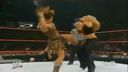
\includegraphics[width=2.4cm]{img/transnetv2/example_detections/0EXCdXUN_fk_001_07058.jpg}};
\node[inner sep=0pt] at (-2.6,0)
{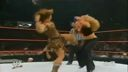
\includegraphics[width=2.4cm]{img/transnetv2/example_detections/0EXCdXUN_fk_001_07059.jpg}};
\node[inner sep=0pt] at (0,0)
{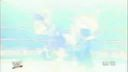
\includegraphics[width=2.4cm]{img/transnetv2/example_detections/0EXCdXUN_fk_001_07060.jpg}};
\node[inner sep=0pt] at (2.6,0)
{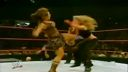
\includegraphics[width=2.4cm]{img/transnetv2/example_detections/0EXCdXUN_fk_001_07061.jpg}};
\node[inner sep=0pt] at (5.2,0)
{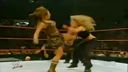
\includegraphics[width=2.4cm]{img/transnetv2/example_detections/0EXCdXUN_fk_001_07062.jpg}};

\draw[-{to reversed[scale=.4]}, thick] (-6.4, -0.85) -- (-2.6, -0.85);
\draw[{to reversed[scale=.4]}-, thick] (0, -0.85) -- (6.4, -0.85);

\draw[dotted] (-6.4, -1) -- (6.4, -1);

\node at (0, -1.1) {};
\end{tikzpicture}



\begin{tikzpicture}
\definecolor{incorrect}{RGB}{255,51,76}
\definecolor{correct}{RGB}{63,188,157}

\node[inner sep=0pt] at (-7.8, 0) {A)};

\node[inner sep=0pt] at (-7.0, 0.52) {\scriptsize GT};
\node[fill=incorrect, inner sep=1.5pt] at (-7.0, 0.22) {\scriptsize NOK};

\node[inner sep=0pt] at (-7.0, -0.18) {\scriptsize Model};
\node[fill=correct, inner sep=1.5pt] at (-7.0, -0.48) {\scriptsize OK};


\node[inner sep=0pt] at (-5.2,0)
{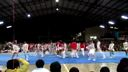
\includegraphics[width=2.4cm]{img/transnetv2/example_detections/Zoj_-rPnxGw_000_00144.jpg}};
\node[inner sep=0pt] at (-2.6,0)
{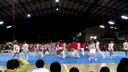
\includegraphics[width=2.4cm]{img/transnetv2/example_detections/Zoj_-rPnxGw_000_00145.jpg}};
\node[inner sep=0pt] at (0,0)
{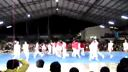
\includegraphics[width=2.4cm]{img/transnetv2/example_detections/Zoj_-rPnxGw_000_00146.jpg}};
\node[inner sep=0pt] at (2.6,0)
{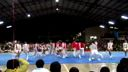
\includegraphics[width=2.4cm]{img/transnetv2/example_detections/Zoj_-rPnxGw_000_00147.jpg}};
\node[inner sep=0pt] at (5.2,0)
{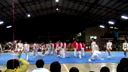
\includegraphics[width=2.4cm]{img/transnetv2/example_detections/Zoj_-rPnxGw_000_00148.jpg}};

\draw[-{to reversed[scale=.4]}, thick] (-6.4, -0.85) -- (-2.6, -0.85);
\draw[{to reversed[scale=.4]}-, thick] (0, -0.85) -- (6.4, -0.85);

\draw[dotted] (-6.4, -1) -- (6.4, -1);

\node at (0, -1.1) {};

\end{tikzpicture}

\begin{tikzpicture}
\definecolor{incorrect}{RGB}{255,51,76}
\definecolor{correct}{RGB}{63,188,157}

\node[inner sep=0pt] at (-7.8, 0) {A)};

\node[inner sep=0pt] at (-7.0, 0.52) {\scriptsize GT};
\node[fill=correct, inner sep=1.5pt] at (-7.0, 0.22) {\scriptsize OK};

\node[inner sep=0pt] at (-7.0, -0.18) {\scriptsize Model};
\node[fill=incorrect, inner sep=1.5pt] at (-7.0, -0.48) {\scriptsize NOK};



\node[inner sep=0pt] at (-5.2,0)
{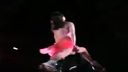
\includegraphics[width=2.4cm]{img/transnetv2/example_detections/7v_BpmoGuPI_000_02058.jpg}};
\node[inner sep=0pt] at (-2.6,0)
{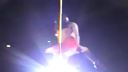
\includegraphics[width=2.4cm]{img/transnetv2/example_detections/7v_BpmoGuPI_000_02059.jpg}};
\node[inner sep=0pt] at (0,0)
{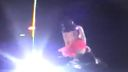
\includegraphics[width=2.4cm]{img/transnetv2/example_detections/7v_BpmoGuPI_000_02063.jpg}};
\node[inner sep=0pt] at (2.6,0)
{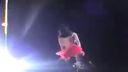
\includegraphics[width=2.4cm]{img/transnetv2/example_detections/7v_BpmoGuPI_000_02067.jpg}};
\node[inner sep=0pt] at (5.2,0)
{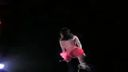
\includegraphics[width=2.4cm]{img/transnetv2/example_detections/7v_BpmoGuPI_000_02069.jpg}};

\draw[thick] (-6.4, -0.85) -- (6.4, -0.85);

\draw[dotted] (-6.4, -1) -- (6.4, -1);

\draw[line width=0.05cm] (-4.6, -1) -- (-3.2, -1);
\draw[line width=0.05cm] (4.6, -1) -- (3.2, -1);


\draw[] (-4.6, -0.92) -- (-4.6, -1.08);
\draw[] (-3.2, -0.92) -- (-3.2, -1.08);
\draw[] (4.6, -0.92) -- (4.6, -1.08);
\draw[] (3.2, -0.92) -- (3.2, -1.08);

\node at (0, -1.1) {};

\end{tikzpicture}


\begin{tikzpicture}
\definecolor{incorrect}{RGB}{255,51,76}
\definecolor{correct}{RGB}{63,188,157}

\node[inner sep=0pt] at (-7.8, 0) {B)};

\node[inner sep=0pt] at (-7.0, 0.52) {\scriptsize GT};
\node[fill=correct, inner sep=1.5pt] at (-7.0, 0.22) {\scriptsize OK};

\node[inner sep=0pt] at (-7.0, -0.18) {\scriptsize Model};
\node[fill=incorrect, inner sep=1.5pt] at (-7.0, -0.48) {\scriptsize NOK};


\node[inner sep=0pt] at (-5.2,0)
{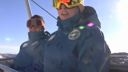
\includegraphics[width=2.4cm]{img/transnetv2/example_detections/-629gOGM1Ic_000_00286.jpg}};
\node[inner sep=0pt] at (-2.6,0)
{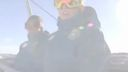
\includegraphics[width=2.4cm]{img/transnetv2/example_detections/-629gOGM1Ic_000_00289.jpg}};
\node[inner sep=0pt] at (0,0)
{
\includegraphics[width=2.4cm]{img/transnetv2/example_detections/-629gOGM1Ic_000_00291.jpg}};
\node[inner sep=0pt] at (2.6,0)
{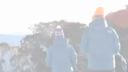
\includegraphics[width=2.4cm]{img/transnetv2/example_detections/-629gOGM1Ic_000_00294.jpg}};
\node[inner sep=0pt] at (5.2,0)
{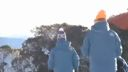
\includegraphics[width=2.4cm]{img/transnetv2/example_detections/-629gOGM1Ic_000_00296.jpg}};

\draw[-{to reversed[scale=.4]}, thick] (-6.4, -0.85) -- (-5.2, -0.85);
\draw[{to reversed[scale=.4]}-, thick] (5.2, -0.85) -- (6.4, -0.85);

\draw[dotted] (-6.4, -1) -- (6.4, -1);

\node at (0, -1.1) {};

\end{tikzpicture}


\begin{tikzpicture}
\definecolor{incorrect}{RGB}{255,51,76}
\definecolor{correct}{RGB}{63,188,157}

\node[inner sep=0pt] at (-7.8, 0) {B)};

\node[inner sep=0pt] at (-7.0, 0.52) {\scriptsize GT};
\node[fill=correct, inner sep=1.5pt] at (-7.0, 0.22) {\scriptsize OK};

\node[inner sep=0pt] at (-7.0, -0.18) {\scriptsize Model};
\node[fill=incorrect, inner sep=1.5pt] at (-7.0, -0.48) {\scriptsize NOK};



\node[inner sep=0pt] at (-5.2,0)
{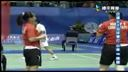
\includegraphics[width=2.4cm]{img/transnetv2/example_detections/5cUViKlaXS8_001_11719.jpg}};
\node[inner sep=0pt] at (-2.6,0)
{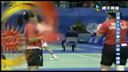
\includegraphics[width=2.4cm]{img/transnetv2/example_detections/5cUViKlaXS8_001_11723.jpg}};
\node[inner sep=0pt] at (0,0)
{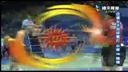
\includegraphics[width=2.4cm]{img/transnetv2/example_detections/5cUViKlaXS8_001_11730.jpg}};
\node[inner sep=0pt] at (2.6,0)
{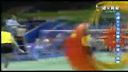
\includegraphics[width=2.4cm]{img/transnetv2/example_detections/5cUViKlaXS8_001_11740.jpg}};
\node[inner sep=0pt] at (5.2,0)
{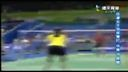
\includegraphics[width=2.4cm]{img/transnetv2/example_detections/5cUViKlaXS8_001_11745.jpg}};


\draw[-{to reversed[scale=.4]}, thick] (-6.4, -0.85) -- (-5.2, -0.85);
\draw[{to reversed[scale=.4]}-, thick] (5.2, -0.85) -- (6.4, -0.85);

\draw[dotted] (-6.4, -1) -- (6.4, -1);

\node at (0, -1.1) {};

\end{tikzpicture}

% \begin{tikzpicture}
% \definecolor{incorrect}{RGB}{255,51,76}
% \definecolor{correct}{RGB}{63,188,157}
% 
% 
% \node[inner sep=0pt] at (-7.0, 0.52) {\scriptsize GT};
% \node[fill=incorrect, inner sep=1.5pt] at (-7.0, 0.22) {\scriptsize NOK};
% 
% \node[inner sep=0pt] at (-7.0, -0.18) {\scriptsize Model};
% \node[fill=correct, inner sep=1.5pt] at (-7.0, -0.48) {\scriptsize OK};
% 
% \node[inner sep=0pt] at (-5.2,0)
% {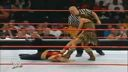
\includegraphics[width=2.4cm]{img/transnetv2/example_detections/0EXCdXUN_fk_000_06299.jpg}};
% \node[inner sep=0pt] at (-2.6,0)
% {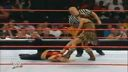
\includegraphics[width=2.4cm]{img/transnetv2/example_detections/0EXCdXUN_fk_000_06300.jpg}};
% \node[inner sep=0pt] at (0,0)
% {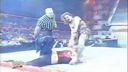
\includegraphics[width=2.4cm]{img/transnetv2/example_detections/0EXCdXUN_fk_000_06301.jpg}};
% \node[inner sep=0pt] at (2.6,0)
% {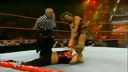
\includegraphics[width=2.4cm]{img/transnetv2/example_detections/0EXCdXUN_fk_000_06302.jpg}};
% \node[inner sep=0pt] at (5.2,0)
% {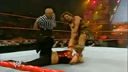
\includegraphics[width=2.4cm]{img/transnetv2/example_detections/0EXCdXUN_fk_000_06303.jpg}};
% 
% \draw[thick] (-6.4, -0.85) -- (6.4, -0.85);
% 
% \draw[dotted] (-6.4, -1) -- (6.4, -1);
% 
% \draw[line width=0.05cm] (0.6, -1) -- (2, -1);
% 
% \draw[] (0.6, -0.92) -- (0.6, -1.08);
% \draw[] (2, -0.92) -- (2, -1.08);
% 
% \node at (0, -1.1) {};
% \end{tikzpicture}

    

\begin{tikzpicture}
\definecolor{incorrect}{RGB}{255,51,76}
\definecolor{correct}{RGB}{63,188,157}

\node[inner sep=0pt] at (-7.8, 0) {C)};

\node[inner sep=0pt] at (-7.0, 0.52) {\scriptsize GT};
\node[fill=incorrect, inner sep=1.5pt] at (-7.0, 0.22) {\scriptsize NOK};

\node[inner sep=0pt] at (-7.0, -0.18) {\scriptsize Model};
\node[fill=correct, inner sep=1.5pt] at (-7.0, -0.48) {\scriptsize OK};


\node[inner sep=0pt] at (-5.2,0)
{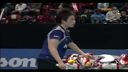
\includegraphics[width=2.4cm]{img/transnetv2/example_detections/1qAzo9Gdw1k_001_00965.jpg}};
\node[inner sep=0pt] at (-2.6,0)
{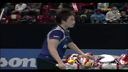
\includegraphics[width=2.4cm]{img/transnetv2/example_detections/1qAzo9Gdw1k_001_00966.jpg}};
\node[inner sep=0pt] at (0,0)
{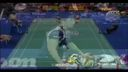
\includegraphics[width=2.4cm]{img/transnetv2/example_detections/1qAzo9Gdw1k_001_00967.jpg}};
\node[inner sep=0pt] at (2.6,0)
{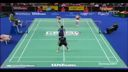
\includegraphics[width=2.4cm]{img/transnetv2/example_detections/1qAzo9Gdw1k_001_00968.jpg}};
\node[inner sep=0pt] at (5.2,0)
{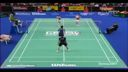
\includegraphics[width=2.4cm]{img/transnetv2/example_detections/1qAzo9Gdw1k_001_00969.jpg}};

\draw[thick] (-6.4, -0.85) -- (6.4, -0.85);

\draw[dotted] (-6.4, -1) -- (6.4, -1);

\draw[line width=0.05cm] (0.6, -1) -- (2, -1);

\draw[] (0.6, -0.92) -- (0.6, -1.08);
\draw[] (2, -0.92) -- (2, -1.08);

\node at (0, -1.1) {};

\end{tikzpicture}
    

% \begin{tikzpicture}
% \definecolor{incorrect}{RGB}{255,51,76}
% \definecolor{correct}{RGB}{63,188,157}
% 
% 
% \node[inner sep=0pt] at (-7.0, 0.52) {\scriptsize GT};
% \node[fill=incorrect, inner sep=1.5pt] at (-7.0, 0.22) {\scriptsize NOK};
% 
% \node[inner sep=0pt] at (-7.0, -0.18) {\scriptsize Model};
% \node[fill=correct, inner sep=1.5pt] at (-7.0, -0.48) {\scriptsize OK};
% 
% 
% \node[inner sep=0pt] at (-5.2,0)
% {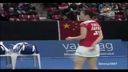
\includegraphics[width=2.4cm]{img/transnetv2/example_detections/1qAzo9Gdw1k_000_00084.jpg}};
% \node[inner sep=0pt] at (-2.6,0)
% {\includegraphics[width=2.4cm]{img/transnetv2/example_detections/1qAzo9Gdw1k_000_00085.jpg}};
% \node[inner sep=0pt] at (0,0)
% {\includegraphics[width=2.4cm]{img/transnetv2/example_detections/1qAzo9Gdw1k_000_00086.jpg}};
% \node[inner sep=0pt] at (2.6,0)
% {\includegraphics[width=2.4cm]{img/transnetv2/example_detections/1qAzo9Gdw1k_000_00087.jpg}};
% \node[inner sep=0pt] at (5.2,0)
% {\includegraphics[width=2.4cm]{img/transnetv2/example_detections/1qAzo9Gdw1k_000_00088.jpg}};
% 
% \draw[thick] (-6.4, -0.85) -- (6.4, -0.85);
% 
% \draw[dotted] (-6.4, -1) -- (6.4, -1);
% 
% \draw[line width=0.05cm] (0.6, -1) -- (2, -1);
% 
% \draw[] (0.6, -0.92) -- (0.6, -1.08);
% \draw[] (2, -0.92) -- (2, -1.08);
% 
% \node at (0, -1.1) {};
% \end{tikzpicture}
    

    

\begin{tikzpicture}
\definecolor{incorrect}{RGB}{255,51,76}
\definecolor{correct}{RGB}{63,188,157}

\node[inner sep=0pt] at (-7.8, 0) {C)};

\node[inner sep=0pt] at (-7.0, 0.52) {\scriptsize GT};
\node[fill=correct, inner sep=1.5pt] at (-7.0, 0.22) {\scriptsize OK};

\node[inner sep=0pt] at (-7.0, -0.18) {\scriptsize Model};
\node[fill=incorrect, inner sep=1.5pt] at (-7.0, -0.48) {\scriptsize NOK};



\node[inner sep=0pt] at (-5.2,0)
{\includegraphics[width=2.4cm]{img/transnetv2/example_detections/5cUViKlaXS8_000_02242.jpg}};
\node[inner sep=0pt] at (-2.6,0)
{\includegraphics[width=2.4cm]{img/transnetv2/example_detections/5cUViKlaXS8_000_02244.jpg}};
\node[inner sep=0pt] at (0,0)
{\includegraphics[width=2.4cm]{img/transnetv2/example_detections/5cUViKlaXS8_000_02245.jpg}};
\node[inner sep=0pt] at (2.6,0)
{\includegraphics[width=2.4cm]{img/transnetv2/example_detections/5cUViKlaXS8_000_02246.jpg}};
\node[inner sep=0pt] at (5.2,0)
{\includegraphics[width=2.4cm]{img/transnetv2/example_detections/5cUViKlaXS8_000_02248.jpg}};

\draw[-{to reversed[scale=.4]}, thick] (-6.4, -0.85) -- (-2.6, -0.85);
\draw[{to reversed[scale=.4]}-, thick] (2.6, -0.85) -- (6.4, -0.85);

\draw[dotted] (-6.4, -1) -- (6.4, -1);

\node at (0, -1.1) {};

\end{tikzpicture}

% \begin{tikzpicture}
% \definecolor{incorrect}{RGB}{255,51,76}
% \definecolor{correct}{RGB}{63,188,157}
% 
% 
% \node[inner sep=0pt] at (-7.0, 0.52) {\scriptsize GT};
% \node[fill=incorrect, inner sep=1.5pt] at (-7.0, 0.22) {\scriptsize NOK};
% 
% \node[inner sep=0pt] at (-7.0, -0.18) {\scriptsize Model};
% \node[fill=correct, inner sep=1.5pt] at (-7.0, -0.48) {\scriptsize OK};
% 
% \node[inner sep=0pt] at (-5.2,0)
% {\includegraphics[width=2.4cm]{img/transnetv2/example_detections/0nZQWIxsLB8_000_01417.jpg}};
% \node[inner sep=0pt] at (-2.6,0)
% {\includegraphics[width=2.4cm]{img/transnetv2/example_detections/0nZQWIxsLB8_000_01418.jpg}};
% \node[inner sep=0pt] at (0,0)
% {\includegraphics[width=2.4cm]{img/transnetv2/example_detections/0nZQWIxsLB8_000_01419.jpg}};
% \node[inner sep=0pt] at (2.6,0)
% {\includegraphics[width=2.4cm]{img/transnetv2/example_detections/0nZQWIxsLB8_000_01420.jpg}};
% \node[inner sep=0pt] at (5.2,0)
% {\includegraphics[width=2.4cm]{img/transnetv2/example_detections/0nZQWIxsLB8_000_01421.jpg}};
% 
% \draw[thick] (-6.4, -0.85) -- (6.4, -0.85);
% 
% \draw[dotted] (-6.4, -1) -- (6.4, -1);
% 
% \draw[line width=0.05cm] (0.6, -1) -- (2, -1);
% 
% \draw[] (0.6, -0.92) -- (0.6, -1.08);
% \draw[] (2, -0.92) -- (2, -1.08);
% 
% \node at (0, -1.1) {};
% 
% \end{tikzpicture}

\begin{tikzpicture}
\definecolor{incorrect}{RGB}{255,51,76}
\definecolor{correct}{RGB}{63,188,157}

\node[inner sep=0pt] at (-7.8, 0) {D)};

\node[inner sep=0pt] at (-7.0, 0.52) {\scriptsize GT};
\node[fill=correct, inner sep=1.5pt] at (-7.0, 0.22) {\scriptsize OK};

\node[inner sep=0pt] at (-7.0, -0.18) {\scriptsize Model};
\node[fill=incorrect, inner sep=1.5pt] at (-7.0, -0.48) {\scriptsize NOK};


\node[inner sep=0pt] at (-5.2,0)
{\includegraphics[width=2.4cm]{img/transnetv2/example_detections/0kzuXD0PmNg_000_06005.jpg}};
\node[inner sep=0pt] at (-2.6,0)
{\includegraphics[width=2.4cm]{img/transnetv2/example_detections/0kzuXD0PmNg_000_06006.jpg}};
\node[inner sep=0pt] at (0,0)
{\includegraphics[width=2.4cm]{img/transnetv2/example_detections/0kzuXD0PmNg_000_06007.jpg}};
\node[inner sep=0pt] at (2.6,0)
{\includegraphics[width=2.4cm]{img/transnetv2/example_detections/0kzuXD0PmNg_000_06008.jpg}};
\node[inner sep=0pt] at (5.2,0)
{\includegraphics[width=2.4cm]{img/transnetv2/example_detections/0kzuXD0PmNg_000_06009.jpg}};

\draw[thick] (-6.4, -0.85) -- (6.4, -0.85);

\draw[dotted] (-6.4, -1) -- (6.4, -1);

\draw[line width=0.05cm] (-0.6, -1) -- (-2, -1);

\draw[] (-0.6, -0.92) -- (-0.6, -1.08);
\draw[] (-2, -0.92) -- (-2, -1.08);

\node at (0, -1.1) {};

\end{tikzpicture}

    

\begin{tikzpicture}
\definecolor{incorrect}{RGB}{255,51,76}
\definecolor{correct}{RGB}{63,188,157}

\node[inner sep=0pt] at (-7.8, 0) {D)};

\node[inner sep=0pt] at (-7.0, 0.52) {\scriptsize GT};
\node[fill=correct, inner sep=1.5pt] at (-7.0, 0.22) {\scriptsize OK};

\node[inner sep=0pt] at (-7.0, -0.18) {\scriptsize Model};
\node[fill=incorrect, inner sep=1.5pt] at (-7.0, -0.48) {\scriptsize NOK};



\node[inner sep=0pt] at (-5.2,0)
{\includegraphics[width=2.4cm]{img/transnetv2/example_detections/-17hVQk3wXI_000_03859.jpg}};
\node[inner sep=0pt] at (-2.6,0)
{\includegraphics[width=2.4cm]{img/transnetv2/example_detections/-17hVQk3wXI_000_03861.jpg}};
\node[inner sep=0pt] at (0,0)
{\includegraphics[width=2.4cm]{img/transnetv2/example_detections/-17hVQk3wXI_000_03862.jpg}};
\node[inner sep=0pt] at (2.6,0)
{\includegraphics[width=2.4cm]{img/transnetv2/example_detections/-17hVQk3wXI_000_03863.jpg}};
\node[inner sep=0pt] at (5.2,0)
{\includegraphics[width=2.4cm]{img/transnetv2/example_detections/-17hVQk3wXI_000_03864.jpg}};

\draw[thick] (-6.4, -0.85) -- (6.4, -0.85);

\draw[dotted] (-6.4, -1) -- (6.4, -1);

\draw[line width=0.05cm] (0.6, -1) -- (2, -1);

\draw[] (0.6, -0.92) -- (0.6, -1.08);
\draw[] (2, -0.92) -- (2, -1.08);

\node at (0, -1.1) {};

\end{tikzpicture}
    
    

\begin{tikzpicture}
\definecolor{incorrect}{RGB}{255,51,76}
\definecolor{correct}{RGB}{63,188,157}
\definecolor{unknown}{RGB}{180,180,180}

\node[inner sep=0pt] at (-7.8, 0) {E)};

\node[inner sep=0pt] at (-7.0, 0.52) {\scriptsize GT};
\node[fill=unknown, inner sep=1.5pt] at (-7.0, 0.22) {\scriptsize ??};

\node[inner sep=0pt] at (-7.0, -0.18) {\scriptsize Model};
\node[fill=unknown, inner sep=1.5pt] at (-7.0, -0.48) {\scriptsize ??};


\node[inner sep=0pt] at (-5.2,0)
{\includegraphics[width=2.4cm]{img/transnetv2/example_detections/6e2-G6CXeT0_000_01253.jpg}};
\node[inner sep=0pt] at (-2.6,0)
{\includegraphics[width=2.4cm]{img/transnetv2/example_detections/6e2-G6CXeT0_000_01254.jpg}};
\node[inner sep=0pt] at (0,0)
{\includegraphics[width=2.4cm]{img/transnetv2/example_detections/6e2-G6CXeT0_000_01255.jpg}};
\node[inner sep=0pt] at (2.6,0)
{\includegraphics[width=2.4cm]{img/transnetv2/example_detections/6e2-G6CXeT0_000_01256.jpg}};
\node[inner sep=0pt] at (5.2,0)
{\includegraphics[width=2.4cm]{img/transnetv2/example_detections/6e2-G6CXeT0_000_01257.jpg}};

\draw[thick] (-6.4, -0.85) -- (6.4, -0.85);

\draw[dotted] (-6.4, -1) -- (6.4, -1);

\draw[line width=0.05cm] (0.6, -1) -- (2, -1);

\draw[] (0.6, -0.92) -- (0.6, -1.08);
\draw[] (2, -0.92) -- (2, -1.08);

\node at (0, -1.1) {};

\end{tikzpicture}

    

\begin{tikzpicture}
\definecolor{incorrect}{RGB}{255,51,76}
\definecolor{correct}{RGB}{63,188,157}
\definecolor{unknown}{RGB}{180,180,180}

\node[inner sep=0pt] at (-7.8, 0) {E)};

\node[inner sep=0pt] at (-7.0, 0.52) {\scriptsize GT};
\node[fill=unknown, inner sep=1.5pt] at (-7.0, 0.22) {\scriptsize ??};

\node[inner sep=0pt] at (-7.0, -0.18) {\scriptsize Model};
\node[fill=unknown, inner sep=1.5pt] at (-7.0, -0.48) {\scriptsize ??};

\node[inner sep=0pt] at (-5.2,0)
{\includegraphics[width=2.4cm]{img/transnetv2/example_detections/-629gOGM1Ic_001_02421.jpg}};
\node[inner sep=0pt] at (-2.6,0)
{\includegraphics[width=2.4cm]{img/transnetv2/example_detections/-629gOGM1Ic_001_02422.jpg}};
\node[inner sep=0pt] at (0,0)
{\includegraphics[width=2.4cm]{img/transnetv2/example_detections/-629gOGM1Ic_001_02423.jpg}};
\node[inner sep=0pt] at (2.6,0)
{\includegraphics[width=2.4cm]{img/transnetv2/example_detections/-629gOGM1Ic_001_02424.jpg}};
\node[inner sep=0pt] at (5.2,0)
{\includegraphics[width=2.4cm]{img/transnetv2/example_detections/-629gOGM1Ic_001_02425.jpg}};

\draw[-{to reversed[scale=.4]}, thick] (-6.4, -0.85) -- (0, -0.85);
\draw[{to reversed[scale=.4]}-, thick] (2.6, -0.85) -- (6.4, -0.85);

\draw[dotted] (-6.4, -1) -- (6.4, -1);

\node at (0, -1.1) {};

\end{tikzpicture}

    \caption[Example TransNet V2 predictions compared to ground truth]{Example TransNet V2 predictions compared to ground truth from the ClipShots test set. The first line below a frame sequence indicates ground truth scenes. The second line indicates the model's prediction (transitions are represented by thick solid line segments, the dotted line means no transition). We indicate the correctness of the ground truth or the predictions by OK/NOK on the left. Some frames were dropped for clarity.}
    \label{fig:transnetv2_predicted_transitions}
\end{figure}




\subsection{Related Work Reevaluation Details}\label{sec:transnetv2Reevaluation}
Hassanien et al. train a neural network with an input of 16 subsequent frames to predict the likelihood of transition anywhere in between the input frames. The network is trained to distinguish between no transition, cut transition, and gradual transition. The network's logit predictions are fed through SVM to predict transitions and color histograms are used to suppress false positives. However, the publicly available code\footnote{Available at \url{https://github.com/melgharib/DSBD}.} only contains the neural network model; therefore, we only use the model without any post-processing. As we do not distinguish between a cut and a gradual transition, we sum their probabilities into one class. To generate per-frame predictions, we assign the predicted transition probability to the middle 8 frames of the 16 frame input sequence and shift the input window every time by 8 frames. Note that our metric is independent of the length of predicted or ground truth transition as long as the prediction overlaps with ground truth at least at one frame. We compute the F1 score for thresholds $\{0.1, 0.2, \dots, 0.9\}$ and use $0.9$ as it produces on average the best F1 score on the test sets. Our method of generating transitions from the predictions achieves a similar result on the RAI dataset as the authors' SVM and color histogram method (93.4\% vs. 93.9\%); therefore, we are confident that its results on ClipShots and BBC datasets objectively represent work of Hassanien et al. Note it is scientifically questionable to select the decision threshold directly on a test set as the achieved results can overestimate the actual model's performance. However, we want to compare ourselves to the best model available; therefore, we accept possible bias in the results. 

Tang et al. utilize a multi-step process for shot boundary detection. However, the only publicly available code\footnote{Available at \url{https://github.com/Tangshitao/ClipShots_basline}.} contains only their ResNet-18 baseline similar to the work of Hassanien et al. When confronting the authors about the code and questionable validation method, we were only pointed to the baseline code; therefore, we evaluate the ResNet-18 baseline and report its results. As the network's input and output are the same as in the case of DeepSBD, the same evaluation method was used with the threshold of $0.8$ achieving the best results.


\subsection{Ablation Study}
We thoroughly investigate our individual design decisions in the following ablation study. Firstly we examine the effect of different types of training data. When conducting the first experiments with TransNet V2, we trained it purely with ClipShots dataset's manually annotated transitions. However, such an approach results in a huge performance drop on both ClipShots and RAI datasets compared to the artificially generated dataset with 50/50 split between hard cuts and dissolves. Therefore, we investigate which type of transition is the most responsible for the performance drop. We substitute half of the real transitions from the training set by hard cuts or dissolves. As can be seen in Table \ref{tb:transnetv2_train_data}, training the model on 50\% real data and 50\% artificially generated hard cuts has almost no effect on the performance while training on real data and artificially generated dissolves bring the model's performance close to the artificial-data-only model. Based on this finding, we conclude it is important for any future work to concentrate efforts on ensuring dissolves are appropriately represented in a train set. Such a conclusion is consistent with the findings of Tang et al., who deliberately extended the ClipShots dataset with additional gradual transitions after observing a weak performance of their model on these transitions.

\begin{table}[h]
	\centering
	\begin{tabular}{l@{\hspace{1cm}}cccc}
		\toprule
		\textbf{Training data} & ClipShots & BBC  & RAI \\
		\midrule
		100\% real transitions                       & $66.4 \pm 1.3$ & $\bm{96.3} \pm 0.5$ & $86.4 \pm 1.2$ \\
		50\% real, 50\% cuts                         & $68.2 \pm 0.7$ & $\bm{96.6} \pm 0.7$ & $84.4 \pm 0.6$ \\
		50\% real, 50\% dissolves                    & $75.3 \pm 0.8$ & $\bm{96.3} \pm 0.5$ & $90.7 \pm 0.7$ \\
		15\% real, 35\% cuts, 50\% dissolves         & $77.0 \pm 0.8$ & $\bm{96.5} \pm 0.5$ & $91.2 \pm 1.1$ \\
		50\% cuts, 50\% dissolves                    & $\bm{77.5} \pm 0.3$ & $95.1 \pm 0.5$ & $\bm{93.2} \pm 0.9$ \\
		\bottomrule
	\end{tabular}
	\caption[Effects of real and artificially generated transitions on TransNet V2 performance]{Effects of real and artificially generated transitions on TransNet V2 performance. Mean F1 scores and standard deviations in percents.}% Computed from 9 model instances (3 best epochs of 3 independent runs as measured on ClipShots validation set).}
	\label{tb:transnetv2_train_data}
\end{table}

Interestingly in Table \ref{tb:transnetv2_train_data} we also see that manually annotated transitions improve performance of the model on BBC Planet Earth -- the dataset that contains high-quality content mostly with plain hard cuts without any peculiar gradual transitions, visual banners or animations commonly present in TV studio broadcast. This is in stark contrast to our initial assumption that real manually annotated transitions would be necessary to detect exotic types of animated transitions as in Figure \ref{fig:transnetv2_predicted_transitions}B but less useful for hard cuts. However, we conclude these exotic transitions are quite uncommon even in the ClipShots dataset, and the added benefit of the real data revolves rather around improving the model's performance on difficult hard cuts.
Even though BBC Planet Earth dataset does not contain extremely dynamic shots, surprisingly, the dataset still includes many difficult hard cuts, as can be seen in Figure \ref{fig:ambiguous_sequence_bbc}. Therefore we train TransNet V2 with 15\% of real transitions, 35\% of artificial hard cuts, and 50\% of artificial dissolves, which still significantly improves model's performance on BBC Planet Earth while achieving similar performance as the artificial-data-only model on the other test sets.


\begin{figure}[h]
    \centering
    \begin{tikzpicture}
    \node[inner sep=0pt] at (-5.2,0)
    {\includegraphics[width=2.4cm]{img/transnetv2/bbc_scene/000.jpg}};
    \node[inner sep=0pt] at (-2.6,0)
    {\includegraphics[width=2.4cm]{img/transnetv2/bbc_scene/001.jpg}};
    \node[inner sep=0pt] at (0,0)
    {\includegraphics[width=2.4cm]{img/transnetv2/bbc_scene/002.jpg}};
    \node[inner sep=0pt] at (2.6,0)
    {\includegraphics[width=2.4cm]{img/transnetv2/bbc_scene/003.jpg}};
    \node[inner sep=0pt] at (5.2,0)
    {\includegraphics[width=2.4cm]{img/transnetv2/bbc_scene/004.jpg}};
    \node at (0, -0.7) {};
    \end{tikzpicture}
    \begin{tikzpicture}
    \node[inner sep=0pt] at (-5.2,0)
    {\includegraphics[width=2.4cm]{img/transnetv2/bbc_scene/100.jpg}};
    \node[inner sep=0pt] at (-2.6,0)
    {\includegraphics[width=2.4cm]{img/transnetv2/bbc_scene/101.jpg}};
    \node[inner sep=0pt] at (0,0)
    {\includegraphics[width=2.4cm]{img/transnetv2/bbc_scene/102.jpg}};
    \node[inner sep=0pt] at (2.6,0)
    {\includegraphics[width=2.4cm]{img/transnetv2/bbc_scene/103.jpg}};
    \node[inner sep=0pt] at (5.2,0)
    {\includegraphics[width=2.4cm]{img/transnetv2/bbc_scene/104.jpg}};
    \node at (0, -0.7) {};
    \end{tikzpicture}
    \begin{tikzpicture}
    \node[inner sep=0pt] at (-5.2,0)
    {\includegraphics[width=2.4cm]{img/transnetv2/bbc_scene/200.jpg}};
    \node[inner sep=0pt] at (-2.6,0)
    {\includegraphics[width=2.4cm]{img/transnetv2/bbc_scene/201.jpg}};
    \node[inner sep=0pt] at (0,0)
    {\includegraphics[width=2.4cm]{img/transnetv2/bbc_scene/202.jpg}};
    \node[inner sep=0pt] at (2.6,0)
    {\includegraphics[width=2.4cm]{img/transnetv2/bbc_scene/203.jpg}};
    \node[inner sep=0pt] at (5.2,0)
    {\includegraphics[width=2.4cm]{img/transnetv2/bbc_scene/204.jpg}};
    %\node at (0, -1.1) {};
    \end{tikzpicture}
    \caption[Difficult hard cuts from BBC Planet Earth dataset]{Difficult hard cuts from BBC Planet Earth dataset. Mind the resolution of the displayed frames is still more than 7 times larger than the network's inputs size ($48\times 27$).}
    %  Courtesy of British Broadcasting Corporation.
    \label{fig:ambiguous_sequence_bbc}
\end{figure}

A natural question is whether our design changes to the original TransNet network are needed to achieve better performance. To answer this, we investigate multiple design decisions -- namely the addition of frame similarity features to the final classifier, shortcuts that effectively halve the shortest path through the convolutional layers, and separable convolutions that factorize large $3\times 3\times 3$ convolution kernels into spatial-only and temporal-only kernels. As seen in Table \ref{tb:key_components_removed}, all design decisions prove to be valuable, especially on more challenging ClipShots dataset where the original TransNet struggles (Table \ref{tb:transnets_results}).

\begin{table}[h]
	\centering
	\begin{tabular}{l@{\hspace{1cm}}cccc}
		\toprule
		\textbf{Model} & ClipShots & BBC  & RAI \\
		\midrule
		TransNet V2                    & $\bm{77.5} \pm 0.3$ & $\bm{95.1} \pm 0.5$ & $93.2 \pm 0.9$ \\
		\midrule
		Without frame similarity       & $77.1 \pm 0.5$ & $94.8 \pm 0.8$ & $\bm{93.5} \pm 0.6$ \\
		Without shortcuts              & $76.9 \pm 0.7$ & $94.8 \pm 0.9$ & $\bm{93.4} \pm 0.5$ \\
		Without separable convolutions & $76.9 \pm 0.6$ & $94.8 \pm 1.4$ & $93.0 \pm 1.2$ \\
		\bottomrule
	\end{tabular}
	\caption[Effect of individual components on the performance of TransNet V2]{Effect of individual components on the performance of TransNet V2. Mean F1 scores and standard deviations in percents computed from 9 model instances.}% Computed from 9 model instances (3 best epochs of 3 independent runs as measured on ClipShots validation set).}
	\label{tb:key_components_removed}
\end{table}

Similarly to the original TransNet, we investigate the effect of the network's depth on performance (Table \ref{tb:transnetv2_depth}). TransNet V2 consists of three SDDCNN V2 blocks, each with two DDCNN V2 cells with skip connection and ended by spatial average pooling, i.e. in total $3\times 2$ DDCNN V2 cells. We increase the depth by adding one more SDDCNN V2 block with twice as many filters as the previous block (512 filters). We also test adding one DDCNN V2 cell in each of three SDDCNN V2 blocks while keeping the number of filters in all SDDCNN V2 blocks the same. Both variants do not perform as well as the $3\times 2$ variant. We hypothesize it is caused by easier over-fitting to the artificial train data -- a phenomenon consistently seen in many of our tests when the number of parameters was increased.

\begin{table}[h]
	\centering
	\begin{tabular}{l@{\hspace{1cm}}cccc}
		\toprule
		\textbf{Model} & ClipShots & BBC  & RAI \\
		\midrule
		TransNet V2                    & $\bm{77.5} \pm 0.3$ & $\bm{95.1} \pm 0.5$ & $\bm{93.2} \pm 0.9$ \\
		\midrule
		$4\times 2$ DDCNN V2 cells     & $77.2 \pm 0.6$ & $94.9 \pm 1.1$ & $91.5 \pm 1.1$ \\
		$3\times 3$ DDCNN V2 cells     & $76.8 \pm 0.8$ & $94.2 \pm 1.3$ & $92.6 \pm 0.9$ \\
		\bottomrule
	\end{tabular}
	\caption[Effect of network's depth on performance]{Effect of network's depth on performance. Mean F1 scores and standard deviations in percents computed from 9 model instances.}
	\label{tb:transnetv2_depth}
\end{table}

As already mentioned in Section \ref{sec:transnetv2DatasetsAugm}, we train the model with additional augmentation techniques to see whether they are necessary to achieve good performance (Table \ref{tb:transnetv2_augmentation}). We observe that the addition of artificial camera shake yields more false negatives than it reduces false positives. Similarly, we see that it is not necessary to generate more types of transitions than the standard hard cuts and dissolves to reach our state-of-the-art results. Finally, we test applying a random color transformation to part of the input frame sequence with a probability of five percent. We see slight improvement on the RAI dataset; however, there is no to a negative effect on ClipShots and BBC Planet Earth.

\begin{table}[h]
	\centering
	\begin{tabular}{l@{\hspace{1cm}}cccc}
		\toprule
		\textbf{Model} & ClipShots & BBC  & RAI \\
		\midrule
		TransNet V2                    & $\bm{77.5} \pm 0.3$ & $\bm{95.1} \pm 0.5$ & $93.2 \pm 0.9$ \\
		\midrule
		%augment all              & $76.5 \pm 0.9$ & $93.8 \pm 1.1$ & $92.9 \pm 1.1$ \\
		Camera shake                   & $76.9 \pm 1.1$ & $94.0 \pm 0.8$ & $93.2 \pm 1.1$ \\
		Wipe transitions               & $76.6 \pm 0.6$ & $94.5 \pm 0.5$ & $92.9 \pm 1.0$ \\
		Random color change            & $77.2 \pm 1.0$ & $94.5 \pm 1.0$ & $\bm{93.8} \pm 0.3$ \\
		\bottomrule
	\end{tabular}
	\caption[Effect of augmentation methods on the performance]{Effect of augmentation methods on the performance. Mean F1 scores and standard deviations in percents computed from 9 model instances.}
	\label{tb:transnetv2_augmentation}
\end{table}

\begin{figure}[h]
    \centering
    \includegraphics[align=c,width=.49\textwidth]{img/pred_transnetv1.jpg}
    \includegraphics[align=c,width=.49\textwidth]{img/pred.jpg}
    \caption[Visual comparison of TransNet and TransNet V2]{Visual comparison of TransNet (left) and TransNet V2 (right). Predictions are shown in green, in blue are shown predictions of the second head of TransNet V2. For example, a transition on the ninth line is detected by TransNet V2 but not by TransNet. The original video authored by Blender Foundation licensed under CC-BY. Some frames skipped due to limited space.}
    \label{fig:transnet_v1_v2_visualization_comparison}
\end{figure}

\chapter{Text-Based Video Retrieval}
With the inception and steady rise of large video collections containing a diverse range of video topics comes the need for fast efficient retrieval. However, even small to medium-size collections are impossible for humans to be browsed manually, especially in a timely manner. Over the years, many sketch-based methods, operating with various visual features, were developed to ease retrieval in these collections \cite{KlausWikiView,BlazekAdam2015,KlausVBS2019_sketchsearch,LokocVBS2019_Nasnet}. Nonetheless, it is inherently difficult, especially for a non-skilled end user, to correctly reproduce a searched object by color, edge, or another sketch. Therefore, recently with advances in deep learning, an option to describe the searched object in natural language gained popularity \cite{SOMHunterVBS2020,LokocVBS2020_VIRET}. %{\color{red} Nonetheless the larger the collections less likely the searched scene is visually distinct to be exactly rememberable and reproducible by a human interacting with the collection. In these cases of zero visual example usually the only option is to describe a query in natural language  COZE ???}.
%We should note that even though an example image can be obtained for example from Google Images it can be completely dissimilar to the searched object in the collection since plethora of images can fit the same description.


Retrieval in video collections by textual queries, also called ad-hoc video search (AVS), represents a great challenge as it is necessary to semantically understand the content of queries and videos. %AVS differs from classical concept detection because in many cases interactions between objects needs to be captured, e.g.
For example, a query \textit{`a person talking behind a podium wearing a suit outdoors after sunset'} requires the system to understand that person is not on the podium and \textit{after sunset} means at night not while the sun is setting. Further, the same information needs to be extracted from the video to retrieve the scene. This example illustrates how AVS differs from classical concept-based retrieval -- rather, it is a combination of concept and action detection, relation modeling, and text understanding.

Since 2016 the ad-hoc video search task is annually held at TRECVid with a goal to model the end-user search use-case. Each year's task consists of 30 one-sentence queries for segments of video containing persons, objects, activities, locations, etc. and combinations of the former.
Until 2018 IACC.3 dataset \cite{2017trecvidawad} of approximately 4600 Internet Archive videos with 600 hours of content was used. In 2019 a larger high-resolution V3C1 dataset \cite{V3C1dataset} of 7475 Vimeo videos with 1000 hours of content was introduced and used onward.

In this chapter, the winning solutions of TRECVid Ad-hoc Video Search 2018 and 2019 are discussed, and a new system built upon work of the 2018 winner Li et al. \cite{XirongW2VVpp} is proposed achieving results on par with the state-of-the-art on TRECVid AVS competition data from years 2016 and 2018. On TRECVid AVS 2017 data, the proposed system improves state-of-art by ten percent showing promising future research direction. Further, the proposed system also outperforms Li et al. on our in-house dataset with over two hundred challenging queries.

\section{Related Work}\label{sec:chap2relatedwork}
%For years content-based retrieval dominated zero-example retrieval... (concept-based video retrieval vs. natural language query)
With the introduction and broad availability of convolutional neural networks for image classification \cite{AlexNet,vgg,Szegedy_2016_InceptionV3}, many works repurposed those networks for concept extraction. 
For example, team NII-HITACHI-UIT \cite{le2016nii}, the winner of TRECVid AVS 2016, utilizes multiple readily available networks for concept detection, scene description as well as dense captioning; therefore, the AVS task is reduced into text-based retrieval task in which similarity scores between query text and video semantic features are computed using inverted index structure and TF-IDF weighting.
These so-called concept-based retrieval systems are, however, limited to only fixed sets of concepts and cannot capture relations between the concepts as the only information available is \textit{present} or \textit{not present} with some confidence measure.

One of the early works that tries to learn directly the matching between images and text is by Wang et al. \cite{Wang2019}. It encodes images into 4096-dimensional vectors using VGG network \cite{vgg}. Sentences are encoded using Word2Vec \cite{word2vec} vectors transformed into 18000-dimensional space using Fisher Vectors. A set of weights is then trained to minimize the distance between these two representations.
Other work by Dong et al. \cite{Dong2018} encodes sentences by concatenating their Bag-of-Words representations, Word2Vec vectors, and RNN outputs. These vectors are then passed through a multi-layer perceptron that is trained together with the RNN to project them into visual feature space created by e.g. ResNet-152. Aside from the text-to-image-space model trained and tested using Flickr30K dataset~\cite{Flickr30k} (containing over 30 thousand images collected from the Flickr website with five captions each), the authors try to learn a text-to-video-space model utilizing MSVD dataset. The video features are extracted using the C3D network and averaged over time; however, better results are achieved by image-based ResNet-152 network instead of the 3D video network.

The above-mentioned approaches represent an image by a single vector that is considered as an aggregation of the important image regions. However, in the process of aggregation, some important information about individual regions can be lost. Lee et al. \cite{Lee_2018_ECCV} introduce Stacked Cross Attention (SCAN), which performs text to image matching by combining similarities between individual image regions and a weighted sum of individual word vectors. Image region vectors are extracted using Faster R-CNN \cite{FasterRCNN} pre-trained on Visual Genomes dataset \cite{krishna2017visual} and one linear trainable layer is added to project the fixed region representations. Word vectors are produced by a trainable bi-directional GRU layer.

\begin{figure}
    \centering
    \includegraphics[width=0.95\textwidth]{img/vlbert_converted.pdf}
    \caption[ViLBERT model for image/description matching]{ViLBERT model \cite{ViLBERT} operates over image regions and text segments. Each stream is a series of transformer and co-attentional transformer layers enabling information exchange between modalities.}
    \label{fig:vlbert}
\end{figure}
ViLBERT \cite{ViLBERT} network by Lu et al. (shown in Figure \ref{fig:vlbert}) takes attention-based approach a step further by repurposing BERT attention-based bidirectional language model \cite{bert}. The original BERT processes each word (token) of an input sentence independently -- the only context is obtained through dozens of attention layers. With pretraining on a large language corpus, BERT and its variants achieved state-of-the-art results in many natural language processing tasks via transfer learning. ViLBERT's input consists of image description and set of image region features that are extracted the same way as in the work Lee et al. The network is pre-trained on large Conceptual Captions \cite{sharma2018conceptual} dataset to predict alignment score i.e. whether an image description matches a set of image regions' features. In the end, the network is finetuned on a manually annotated high-quality Flickr30K dataset. The finetuning is performed by computing the alignment score for the correct image-text pair and other three sampled incorrect pairs. The scores are passed through softmax, and cross-entropy loss is computed. The twelve attention layers in ViLBERT outperform SCAN with only one attention in image retrieval on the Flickr30K dataset by almost 20\% in terms of Recall@1 (recall at the first position) and by over 7\% in Recall@10.

As mentioned by Dong et al., simply exchanging 2D features from networks such as ResNet for 3D features extracted by e.g. C3D is not sufficient to perform video retrieval. Moreover, they imply that video retrieval can be performed with better results by extracting only 2D features. However, it is unfortunate that, by operating only on single frames, some information about actions, etc. is inevitably lost. Work of Mithun et al. \cite{Mithun2018} argues that 3D video features such as I3D and 2D image features produced by e.g. ResNet focus on different characteristics and are complementary in some sense. The first focuses on action identification and the later on identifying objects in the frames. Therefore the authors introduce two spaces: activity-text space and object-text space. A text query is then evaluated in both spaces independently, and the fusion of those two rankings is performed. Nonetheless, work of Yu et al. \cite{Yu_2018_ECCV} utilizing again only image-based ResNet-152 for feature extraction outperforms Mithun et al. by 45\% for both Recall@1 and Recall@10 in video retrieval task on MSR-VTT \cite{Xu_2016_CVPR} dataset (containing 10 thousand web video videos with 200 thousand short clips each paired with text descriptions).

\subsection{Weakly Supervised Approaches}
\begin{figure}
    \centering
    \begin{equation}\label{eg:maxmarginrankingloss}
        \begin{split}
        \min\sum_{i=1}^{|\mathcal{B}|} \left( \sum_{j\in \mathcal{N}(i)}\right. [\delta & + S(V_i,C_j) - S(V_i,C_i)]_+ \\
        & \left. + \sum_{j\in \mathcal{N}(i)} [\delta + S(V_j,C_i) - S(V_i,C_i)]_+ \right)
        \end{split}
        % \min\sum_{j\in \mathcal{N}(i)}\left(\left[\delta + S(V_i,C_j) - S(V_i,C_i)\right]_+ + \left[\delta + S(V_j,C_i) - S(V_i,C_i)\right]_+\right)
    \end{equation}
    \begin{equation}
        \max\ \sum_{i=1}^{|\mathcal{B}|} \log \left(\frac{e^{S(V_i, C_i)}}{e^{S(V_i, C_i)}+\sum_{j \in \mathcal{N}(i)} \left[e^{S(V_i, C_j)} + e^{S(V_j, C_i)}\right]}\right)\label{eg:nceloss}
    \end{equation}
    
    \caption[Max-margin ranking loss and noise-contrastive estimation loss.]{Max-margin ranking loss and noise-contrastive estimation loss. $S(V_i,C_j)$ is a similarity score between video clip $V_i$ and caption $C_j$, $\mathcal{N}(i)$ is a set of negatives for video/caption $i$, $\delta$ is the margin and $\left[\cdot\right]_+$ is $max(0, \cdot)$. In \cite{Miech_2020_CVPR} authors allow for multiple positive pairs $\mathcal{P}(i)$ due to uncertainty in video-caption alignment by substituting $e^{S(V_i, C_i)}$ for $\sum_{(x,y)\in\mathcal{P}(i)}e^{S(V_x, C_y)}$.}
\end{figure}

Learning mappings of text and videos into joint embedding space often requires large manually annotated datasets. Even though there are datasets such as MSR-VTT or Tumblr GIF (TGIF) \cite{Li_2016_CVPR}, each with more than 100 thousand short clips (or gifs in the latter case) with their natural language descriptions, the work of Miech et al. \cite{Miech_2019_ICCV_HowTo100M} shows that even much larger datasets are greatly beneficial to video retrieval. The authors introduce HowTo100M dataset containing 136 million video clips from 1.22 million narrated instructional web videos, each accompanied by automatically or human-generated audio transcriptions. Although the transcriptions need not to align with the visual content or they may be unrelated completely, a simple shallow network trained max-margin ranking loss (Equation \ref{eg:maxmarginrankingloss}) achieves state-of-the-art results on multiple benchmarks.
For video, the network utilizes 2D and 3D features extracted by Resnet-152 pre-trained on ImageNet and ResNeXt-101 pre-trained on Kinetics respectively. The features are then aggregated by temporal max-pooling and concatenated. Transcriptions are embedded using Word2Vec and a shallow 1D convolutional network is used to extract fixed-sized representation. Further, a single linear fully-connected layer with a two-layer context gating function is used for both the visual and textual features. The authors stress that, during training, intra-video negative sampling strategy is critical for good performance -- half of the negative pairs in the loss belong to the same original video to ensure that the learned embedding focuses on relevant aspects of the video clip.

In video retrieval task on the MSR-VTT dataset, this network achieves very similar results as Mithun et al.; however, the network is only trained on HowTo\-100M. Finetuning on MSR-VTT improves the results of Mithun et al. by more than 110\% in Recall@1 and 77\% in Recall@10. Additional work by the authors \cite{Miech_2020_CVPR} shows the benefits of training video feature extractors (I3D or S3D) from scratch. Further it is suggested that noise-contrastive estimation loss (\cite{ExploringLimitsLanguageModeling}, Equation \ref{eg:nceloss}) outperforms standard max-margin ranking loss.


\subsection{Winners of TRECVid Ad-hoc Video Search}\label{sec:winnersOfTrecvid}
This section summarizes approaches used by winning teams of TRECVid AVS challenge. Namely, it focuses on Dual Encoding by Dong et al. \cite{Dong_2019_CVPR} and Word-To-Visual-Vector (W2VV++) by Li et al. \cite{XirongW2VVpp} (shown in Figure \ref{fig:w2vvpp_original_sketch}) since these have been used in the winning submissions of 2018 and 2019 \cite{wu2019hybrid, li2018renmin, li2019renmin}.


\begin{figure}
    \centering
    \includegraphics[width=0.6\textwidth]{img/w2vvpp_converted.pdf}
    \caption[A diagram of W2VV++ model]{A diagram of the original version of W2VV++ model, taken from \cite{XirongW2VVpp}.}
    \label{fig:w2vvpp_original_sketch}
\end{figure}

\begin{description}[labelwidth=1em, leftmargin=!]
    \item \textbf{Frame features.} Image-based 2D CNNs are used to extract features for individual frames. In particular Li et al. utilizes two CNNs: ResNeXt-101 from \cite{ImageNetShuffle} and ResNet-152 from MXNet library \cite{mxnet} %\cite{DL-61-86 at TRECVID 2017: Video-to-Text Description}
    both trained on the ImageNet dataset with over 10 million images and over 10 thousand classes.
    Frames are resized to $256\times 256$ and CNN features (the output of the penultimate layer) are extracted from its 10 sub-images (i.e. five $224\times 224$ center and corner patches, all of them also horizontally flipped). The final frame features are the result of averaging those ten sub-image features and concatenation of ResNeXt-101 and ResNet-152 features.

    \item \textbf{Video features.} For a given video clip frames are sampled every 0.5 seconds. Features for each frame are extracted as described above. Then the features are aggregated by one or more of the following approaches: (1) averaging features over time. (2) using a bidirectional recurrent neural network with e.g. GRU units with outputs of both directions concatenated and averaged over time. (3) using 1D convolution with outputs averaged over time. (4) computing differentiable version of VLAD (Vector of Locally Aggregated Descriptors) -- NetVLAD \cite{Arandjelovic_2016_CVPR}. (5) using graph network \cite{Mao_2018_ECCV_Workshops} to learn a fixed-sized hierarchical representation of the video among frames.
    
    Wu et al. \cite{wu2019hybrid} utilize averaging over time (1). Further GRU (2), NetVLAD (4), graph network (5) are run in parallel on top of frame features.
    Video representation of Dong et al. \cite{Dong_2019_CVPR} concatenates output of the approach (1), GRU (2) and 1D CNN (3) run on top of the GRU features. Li et al. \cite{XirongW2VVpp} use only the feature averaging over time.
    
    \item \textbf{Word features.} Over the years multiple approaches to word embeddings have been developed. All three mentioned works adopt a pre-trained 500-dimensional Word2Vec model trained on English tags associated with 30 million Flickr images supporting over 1.7 million words \cite{Dong2018}. The 2019 version \cite{li2019renmin} of W2VV++ system by Li et al. also takes advantage of pre-trained BERT \cite{bert} sub-word embeddings.
    
    \item \textbf{Sentence features.} One of the simplest representation is bag-of-words (BoW). The work of Li et al. constructs BoW by taking all words from a training set, excluding those that occur less than five times and those contained in the NLTK stopword list. Aside from the BoW features, Li et al. utilize Word2Vec pre-trained embeddings and single layer 1024-dimensional GRU network. The outputs of both methods are averaged over all words and concatenated together with BoW into $(500+1024+11147)$-dimensional vector. %The 2019 version also adds 1024-dimensional pre-trained BERT embeddings also averaged over all input tokens.
    Works of Wu et al. and Dong et al. embed words using the Word2Vec pre-trained embeddings and use the same architecture as they use for video feature extraction. Further, they also allow to fine-tune the embeddings.
    
    \item \textbf{Loss function.} Li et al. and Dong et al. project sentence features and video features into the common vector spaces by a single fully-connected layer followed by hyperbolic tangent or batch normalization respectively. Then all the approaches adopt max-margin ranking loss (Equation \ref{eg:maxmarginrankingloss}) with hard negatives \cite{VSEpp}, i.e. $\mathcal{N}(i)=\textrm{argmax}_{j\neq i} S(V_i, C_j)$ or $\textrm{argmax}_{j\neq i} S(V_j, C_i)$ for the first and the second term respectively. The idea behind the hardest negative can be intuitively explained by the fact that the hardest negative determines success or failure in the Recall@1 metric. For practical reasons, the hardest negative is selected only from mini-batch instead of the whole dataset. The work of Li et al. further only uses the second term in the max-margin ranking loss with negatives for videos but not for sentences.
    % \item \textbf{Train, validation and test sets.}
\end{description}



\clearpage
\section{Our Method}\label{sec:chap2ourmethod}
As already mentioned, text-to-visual matching systems usually employ pre-\linebreak[4]trained visual and text feature extractors and learn only the mapping between these features. While some work focuses on training video feature extractors \cite{Miech_2020_CVPR}, to the best of our knowledge, no work trains advanced text feature extractors. The authors of \cite{Miech_2020_CVPR} prove that training the whole video extractor benefits from the performance if large, even only automatically annotated, datasets are available. In this work, we experimentally prove the same for the text extractor. For that we adopt Transformer-based \cite{AttentionisAllyouNeed} state-of-the-art model RoBERTa \cite{RoBERTa}, pre-trained on large corpora of English texts from the internet such as Wikipedia and news articles. Even though Transformers have already been used in the text-to-visual systems, e.g. Renmin University at TRECVid 2019 \cite{li2019renmin} and Contrastive Bidirectional Transformer \cite{ContrastiveBidirectionalTransformer} both utilized pre-trained BERT or Miech et al. \cite{Miech_2020_CVPR} adopted one Transformer's attention layer into their language part of the system; we show that training the whole Transformer network for this task is beneficial.

\subsection{Problem Statement} Given a video $V=\{v_1, \ldots, v_n\}$ with frames $v_i$ and a text caption $C=\{c_1,\ldots,c_m\}$ with words $c_i$, we aim to learn a mapping of the video $f(V; \theta_f)$ into $\R^d$ and a mapping of the caption $g(C; \theta_g)$ to the same space $\R^d$ such that similarity $S(V, C)$ is maximized for a video-caption pair, if the caption describes correctly the video, and minimized for a pair, if the caption does not describe the video. Note, we will omit the parameters $\theta_f$ or $\theta_g$ and refer to both the functions and their parameters by only $f$ or $g$ for simplicity. We define the similarity as cosine of $f(V)$ and $g(C)$ as
\begin{equation}
    S(V, C)=\frac{f(V)^\top g(C)}{\|f(V)\|_2\|g(C)\|_2}.
\end{equation}

In this framework, text retrieval in a video database $\mathcal{DB}$ is solved by computing $f(V_i)$ for all videos $V_i$. Given a query $Q$, $g(Q)$ is computed and for each video similarity scores $S(V_i, Q)$ are computed and the videos with the highest scores are returned. Since $f(V_i)$ can be precomputed and $g(Q)$ can be considered as a constant for a query of limited length, the time complexity is determined by the size of the database and the dimension $d$ of the joint space $\R^d$, i.e. $O(|\mathcal{DB}|d)$. Note, in practice, a video can contain many unrelated segments while the query usually describes only one segment; therefore, videos are split into individual shots, i.e. in the context of this thesis $V_i$ is not the whole video but only a single shot.


\subsection{Video Representation}
For video representation we use the W2VV++ (Word-To-Visual-Vector) system~\cite{XirongW2VVpp} developed by Li et al. As described in Section \ref{sec:winnersOfTrecvid} a frame is extracted every 0.5 seconds, it is resized into $256\times 256$ and features are extracted from its 10 sub-images. The features are obtained by ResNext-101 \cite{ImageNetShuffle} and Resnet-152 \cite{mxnet} both trained on ImageNet. The features are averaged across the image patches and all the video frames resulting in a fixed 4096-dimensional vector.

The only trainable part of the video mapping function $f$ is a single fully-connected layer with hyperbolic tangent, i.e. the whole video mapping function is as follows:
\begin{equation}
    f(V)=\tanh\left(W_f\mathcal{N}(V)+b_f\right)
\end{equation}
where $\mathcal{N}(\cdot)$ is the non-trainable mapping to 4096-dimensional space by CNNs averaged over frames described in the previous paragraph, $W_f\in\R^{d\times 4096}$ and $b_f\in \R^d$ are the trainable weights and biases.

\subsection{Text Representation}
Similarly to Li et al. three components are utilized -- Bag of Words, Word2Vec, and newly BERT instead of RNN. Specifically, the Bag of Words component is defined as
\begin{equation}
    BoW(C)=\left(\#(w_1, C),\ldots,\#(w_{|\mathcal{V}|}, C)\right)
\end{equation}
where $w_i\in\mathcal{V}$ are words from a vocabulary and $\#(w,C)$ is number of occurrences of a word $w$ in the text $C$. We use the same vocabulary as Li et al. with $|\mathcal{V}|=11147$ words.

Word2Vec component utilizes a pre-trained 500-dimensional model trained on English tags associated with 30 million Flickr images supporting over 1.7 million words \cite{Dong2018}. A text caption $C$ is represented by the average of the individual word embeddings $e(c_i)$. The embedding is not fine-tuned and stays fixed throughout the whole training.
\begin{equation}
    W2V(C)=\frac{1}{|C|}\sum_{i=1}^{|C|}e(c_i)
\end{equation}

The last component of the text architecture is BERT neural network \cite{bert}. BERT's architecture is a multi-layer bidirectional Transformer encoder based on the work by Vaswani et al. \cite{AttentionisAllyouNeed} (Figure \ref{fig:original_bert}). It uses only self-attention and point-wise, fully connected layers stacked into transformer blocks with information passing between words (sub-words) only via the self-attention. In our work, we use the 110 million parameter variant of BERT called $\mathrm{BERT_{BASE}}$ with 12 Transformer blocks, size of the hidden layers 768, and 12 self-attention heads. For detailed architecture description, we point readers to the original work of Vaswani et al.~\cite{AttentionisAllyouNeed} and the BERT paper \cite{bert}.

BERT outputs a 768-dimensional vector for each input sub-word. We average all sub-word vectors to obtain representation $BERT(C)$ of the original text caption $C$.
We initialize BERT's weights by the ones provided by the authors of \textit{RoBERTa: A Robustly Optimized BERT Pretraining Approach} \cite{RoBERTa} and further train them on our dataset.

Similarly to the video network, the text network $g$ ends by concatenating the text representations and applying a fully-connected layer with hyperbolic tangent and projects a text caption into the joint text-video space:
\begin{equation}
    g(C)=\tanh\left(W_g\left[BoW(C); W2V(C); BERT(C)\right]+b_g\right).
\end{equation}
In the equation, $\left[\ldots\right]$ is vector concatenation, $W_g\in\R^{d\times (11147+500+768)}$ and $b_f\in \R^d$ together with all the weights of BERT are the trainable parameters of $g$.

\begin{figure}
    \centering
    \newcolumntype{C}[1]{>{\centering\arraybackslash}p{#1}}
    \begin{tabular}{cC{0.7cm}cC{0.7cm}c}
    \includegraphics[align=c,width=.2\textwidth]{img/bert/bert.png}
    &
    &
    \includegraphics[align=c,width=.25\textwidth]{img/bert/bert-attention.png}
    &
    &
    
    \includegraphics[align=c,width=.15\textwidth]{img/bert/bert-singleattention.png}
    \end{tabular}
    \caption[Schema of Transformer-based encoder such as BERT]{Schema of Transformer-based encoder such as BERT (left), multi-head attention (middle), and single scaled dot-product attention (right). Images from \cite{AttentionisAllyouNeed}.}
    \label{fig:original_bert}
\end{figure}

\subsection{Loss Function}
Our work employs the same variant of max-margin ranking loss (Equation \ref{eg:maxmarginrankingloss}) as Li et al. Specifically, the term with caption negatives is ignored and the set of video negatives contains only the hardest negative from a batch $\mathcal{B}$:
\begin{equation}\label{eq:our_loss}
    \min\sum_{i=1}^{|\mathcal{B}|}\left[\delta + \textrm{argmax}_{j\neq i} S(V_j, C_i) - S(V_i,C_i)\right]_+.
\end{equation}
We discuss the decision and compare other losses in the next section.



\clearpage
\section{Experiments}\label{sec:chap2experiments}
We first describe datasets used in our experiments for training, validation, and testing together with metrics used for evaluation. Then in Section \ref{sec:trainingDetails} training details are provided. Section \ref{sec:chap2results} presents the results of our model and compares them to the related work, mainly W2VV++ \cite{XirongW2VVpp}. Finally, an ablation study in Section \ref{sec:chap2ablation} justifies key design choices such as the loss function.

\subsection{Datasets and Evaluation Metrics}
We use the same train, validation and test sets as in the work of Li et al. with the features provided by the authors\footnote{\label{note:1}Publicly available at \url{https://github.com/li-xirong/avs}.}. For train set MSR-VTT \cite{Xu_2016_CVPR} and Tumblr GIF (TGIF) \cite{Li_2016_CVPR} is used. TGIF dataset contains over 100 thousand animated GIFs with their natural language captions. MSR-VTT dataset contains 200 thousand short clips each paired with text descriptions in 10 thousand videos.
For validation is used TRECVID 2016 Video-to-Text task dataset \cite{awad2016trecvid} with two thousand Vine videos each described by a sentence by two annotators. To stay consistent with Li et al. we utilize only 200 videos provided by the authors\footref{note:1}.
Testing is performed on the IACC.3 dataset \cite{2017trecvidawad} used for TRECVid AVS task from 2016 to 2018 containing approximately 4600 Internet Archive videos with 600 hours of content. The videos are split into 335,944 short clips by automatically detected shot boundaries provided by the authors of the dataset.
Further for testing we use over two hundred sentence-based queries manually collected for 20 thousand frames uniformly sampled from the V3C1 dataset (dubbed 20k-V3C1).

Suppose we have a set $\mathcal{Q}=\{\left(C_i,\mathcal{T}_i\right)\}_i$ of caption-video pairs with the possibility that a caption $C_i$ can correspond to many target videos $V\in\mathcal{T}_i$. Given a query (text caption) $C$ a model asigns each video $V$ a position (rank) in the result list $r(C, V)$. Good model will assign low $r(\cdot, \cdot)\to 1$ for relevant videos and large $r(\cdot, \cdot)\to |\mathcal{DB}|$ for irrelevant ones. We use the following metrics to measure model performance. Recall@k (R@k) is defined as:
\begin{equation}
    \mathrm{Recall@k}=\frac{1}{|\mathcal{Q}|}\sum_{\left(C_i,\mathcal{T}_i\right)\in \mathcal{Q}}\left(\frac{1}{|\mathcal{T}_i|}\sum_{V\in \mathcal{T}_i} [\![r(C_i,V)\leq k]\!]\right)
\end{equation}
where $[\![\cdot]\!]$ is indicator function which is one if the argument is true and zero otherwise. As we use Recall@k in scenario where there is always only a single target video ($\mathcal{T}_i=\{V_i\}$) the expression in the bracket can be simplified into $[\![r(C_i,V_i)\leq k]\!]$.
Further, the official TRECVid AVS metric is based on mean average precision (mAP). The standard mAP is defined as:
\begin{equation}
    \mathrm{mAP}=\frac{1}{|\mathcal{Q}|}\sum_{\left(C_i,\mathcal{T}_i\right)\in \mathcal{Q}}\left(\frac{1}{|\mathcal{T}_i|}\sum_{V\in \mathcal{T}_i}
    \frac{\left|\{\nu\in\mathcal{T}_i\ |\ r(C_i,\nu)\leq r(C_i,V)\}\right|}{r(C_i,V)}\right)
\end{equation}
where the innermost fraction is Precision@k with $k=r(C_i,V)$. If the set of target videos $\mathcal{T}_i$ contains only one video $V_i$ the metric is also called mean reciprocal rank (MRR) $1/|\mathcal{Q}|\cdot\sum_{\left(C_i,\{V_i\}\right)\in \mathcal{Q}}1/r(C_i,V_i)$.


Since it is difficult to evaluate all 335,944 shots from IACC.3 manually, performance at TRECVid AVS task is measured by inferred average precision (infAP) \cite{infAP}. Compared to standard (mean) average precision it eliminates bias created by only manually labeling the retrieved shots while unretrieved shots are not labeled.

\subsection{Training Details}\label{sec:trainingDetails}
In all our experiments, unless otherwise stated, the joint space dimension $d$ is set to $2048$.
Prior training, weights $W_f$ and $W_g$ are initialized by Glorot initiali\-zer~\cite{Xavier_Glorot_init}, biases $b_f$ and $b_g$ are initialized by zeros and BERT network by pre-trained weights from \cite{RoBERTa}. Batch size of 96 clip-text pairs is selected to fit into 16GB of VRAM of a Tesla V100 GPU. We use the Adam optimizer \cite{Adam14} with a learning rate of $10^{-5}$ and linear warm-up for the half of the first epoch (approx. 1700 steps). The learning rate is linearly decayed to zero in a span of 60 epochs; however, the best performing model on the validation set is selected which is usually achieved after approximately ten epochs. With the video features extracted beforehand, the training itself takes a few hours on a single Tesla V100 GPU. Pytorch and its fairseq\footnote{Available at https://github.com/pytorch/fairseq} library with the implementation of BERT has been used for all the experiments.

\subsection{Results}\label{sec:chap2results}
We report the results of three variants: A) the whole model as described in Section \ref{sec:chap2ourmethod} is used. B) the Word2Vec portion of the text encoding network is removed. C) both Word2Vec and Bag-of-Words parts of the text network are removed, i.e. only BERT is used for text projection into the joint space. Similarly, we report results of the original W2VV++ \cite{XirongW2VVpp} as well as W2VV++ with only Bag-of-Words in the text network, i.e. without Word2Vec and RNN.

Table \ref{tb:general_results} shows the performance of various models on TRECVid AVS tasks for years 2016 through 2018. We see slightly lower performance of our BERT based systems on 2016 and 2018 tasks while we see significantly better results for 2017 tasks. A single model combining BERT, Word2Vec, and Bag-of-Words even outperforms the second-best performer of TRECVid AVS 2019 challenge both in single model setting (infAP 22.8) and also in an ensemble setting where multiple Dual Encoding models were combined to produce the result (infAP 23.9 \cite{li2019renmin}). Surprisingly the original W2VV++ system is outperformed by its BoW-only variant in all three years. We hypothesize it is due to the fact that (inferred) mean average precision heavily favors results with the target item in the first position. For example, a model returning a target item always in the top 10 results can achieve worse mAP than a model returning a target item a few times at the first position but other times not returning it at all.

\begin{table}
	\centering
	\sisetup{detect-weight=true,detect-inline-weight=math}
	\begin{tabular}{l@{\hspace{1cm}}S[table-format=2.1]S[table-format=2.1]S[table-format=2.1]S[table-format=2.1]}
		\toprule
		\textbf{Model} & \multicolumn{1}{c}{TV16} & \multicolumn{1}{c}{TV17}  & \multicolumn{1}{c}{TV18} & \multicolumn{1}{c}{Average} \\
		\midrule
		W2VV++ \cite{XirongW2VVpp}            & 15.5 & 21.5 & 10.7 & 15.9 \\
		W2VV++ (BoW only)\textsuperscript{$*$}& \bftabnum 15.6 & 21.8 & \bftabnum 11.0 & 16.1 \\
		\textbf{Ours} (BERT)                  & 13.7 & 22.5 & 09.8 & 15.3 \\
		\textbf{Ours} (BERT + BoW)            & 15.0 & 23.4 & 10.3 & 16.2 \\
		\textbf{Ours} (BERT + BoW + Word2Vec) & 14.6 & \bftabnum 24.1 & 10.2 & \bftabnum 16.3 \\
		\midrule
		Dual Encoding \cite{Dong_2019_CVPR}\textsuperscript{$\dagger$} & \bftabnum 16.5 & 22.8 & \bftabnum 11.7 & \bftabnum 17.0  \\
		\bottomrule
		\multicolumn{5}{l}{\footnotesize \textsuperscript{$*$} W2VV++ utilizes BoW, Word2Vec and RNN, this version uses only BoW.} \\
		\multicolumn{5}{l}{\footnotesize \textsuperscript{$\dagger$} Results taken from \cite{li2019renmin}.} \\
	\end{tabular}
	\caption[Model comparison on TRECVid AVS tasks]{Model comparison on TRECVid AVS tasks for years 2016 to 2018. Values are in percents of inferred mean average precision averaged over three runs. Results for W2VV++ are courtesy of the authors.}
	\label{tb:general_results}
\end{table}

The described phenomenon can be seen in results on the 20k-V3C1 dataset show in Table \ref{tb:20k_results}. BoW-only variant of W2VV++ retrieves the searched frame at the first position in almost twelve percent of 202 sentence based queries. However, when we look at the percentage of queries such that the target frame is retrieved in the top ten positions, BoW-only W2VV++ already performs the worst of all the models. Further, the difference can be seen for the top 100 positions where our model outperforms BoW-only W2VV++ by almost 11 percentage points. Also visual comparison of the full W2VV++ model and our BERT extension can be seen in Figures \ref{fig:w2vv_bert_comparison_bertbetter}, \ref{fig:w2vv_bert_comparison_w2vvbetter} and \ref{fig:w2vv_bert_comparison_wrong}.

\begin{table}
	\centering
	\sisetup{detect-weight=true,detect-inline-weight=math}
	\begin{tabular}{l@{\hspace{1cm}}S[table-format=2.1]S[table-format=2.1]S[table-format=2.1]S[table-format=2.1]S[table-format=2.1]}
		\toprule
		\textbf{Model} & \multicolumn{1}{c}{R@1} & \multicolumn{1}{c}{R@10} & \multicolumn{1}{c}{R@100} & \multicolumn{1}{c}{MRR}\\
		\midrule
		W2VV++ \cite{XirongW2VVpp}            &  7.9 & 28.7 & 60.4 & 14.6 \\
		W2VV++ (BoW only)                     & \bftabnum 11.9 & 27.2 & 57.4 & \bftabnum 16.5 \\
		\textbf{Ours} (BERT)                  &  8.9 & 28.2 & 65.3 & 14.8\\
		\textbf{Ours} (BERT + BoW)            &  9.9 & 27.2 & 65.8 & 16.1\\
		\textbf{Ours} (BERT + BoW + Word2Vec) &  9.4 & \bftabnum 30.2 & \bftabnum 68.3 & 16.4\\
		\bottomrule
	\end{tabular}
	\caption[Model comparison on 20k-V3C1 dataset]{Model comparison on 20k-V3C1 dataset (20k frames, 202 frame-caption pairs). Recall@k and mean reciprocal rank shown in percents. Note R@100 represents recall given 0.5 percent of the original dataset.}
	\label{tb:20k_results}
\end{table}

In Table \ref{tb:tv16vtt} results on TRECVid 2016 Video-to-text dataset are shown. Note the dataset was used for validation in our experiments as well as experiments of Li et al. Every video in the dataset is captioned by two annotators -- hence the set A and set B. For validation purposes only the set A was used. The results show that all our models outperform both W2VV++ variants in all metrics. Surprisingly the BERT-only model outperforms the other combinations.

\begin{table}
	\centering
	\sisetup{detect-weight=true,detect-inline-weight=math}
	\begin{tabular}{l@{\hspace{0.2cm}}S[table-format=2.1]S[table-format=2.1]S[table-format=2.1]S[table-format=2.1]S[table-format=2.1]S[table-format=2.1]}
		\toprule
		\multirow{2}{*}{\textbf{Model}} & \multicolumn{3}{c}{Set A} & \multicolumn{3}{c}{Set B} \\
		& \multicolumn{1}{c}{R@1} & \multicolumn{1}{c}{R@10} & \multicolumn{1}{c}{MRR} & \multicolumn{1}{c}{R@1} & \multicolumn{1}{c}{R@10} & \multicolumn{1}{c}{MRR}\\
		\midrule
		W2VV++ \cite{XirongW2VVpp}            & 42.5 & 79.0 & 55.7 & 43.0 & 82.5 & 56.9 \\
		W2VV++ (BoW only)                     & 39.5 & 79.0 & 52.3 & 41.0 & 82.0 & 54.3 \\
		\textbf{Ours} (BERT)                  & \bftabnum 45.0 & 82.0 & \bftabnum 58.4 & \bftabnum 47.5 & \bftabnum 86.5 & \bftabnum 59.0 \\
		\textbf{Ours} (BERT + BoW)            & 43.0 & \bftabnum 82.5 & 56.3 & 45.5 & 85.0 & 57.8 \\
		\textbf{Ours} (BERT + BoW + W2V)      & 43.5 & 80.5 & 57.1 & 45.0 & 82.5 & 57.0 \\
		\bottomrule
	\end{tabular}
	\caption[Model comparison on TRECVid 2016 Video-to-text dataset]{Model comparison on TRECVid 2016 Video-to-text dataset.}
	\label{tb:tv16vtt}
\end{table}



\subsection{Ablation Study}\label{sec:chap2ablation}
We perform multiple ablation studies. In Table \ref{tb:max_margin_loss_variants} we compare our text-to-visual max-margin ranking loss (Equation \ref{eq:our_loss}) to bidirectional (text-to-visual + visual-to-text) variant that minimizes not only similarity of hardest negative video to a caption but also similarity of hardest negative caption to a video (adaptation of Equation \ref{eg:maxmarginrankingloss}). We see slightly better results for the text-to-visual version of the loss on TRECVid AVS tasks with our full model (BERT + BoW + W2V).

\begin{table}
	\centering
	\sisetup{detect-weight=true,detect-inline-weight=math}
	\begin{tabular}{l@{\hspace{1cm}}S[table-format=2.1]S[table-format=2.1]S[table-format=2.1]S[table-format=2.1]}
		\toprule
		\textbf{Loss} & \multicolumn{1}{c}{TV16} & \multicolumn{1}{c}{TV17}  & \multicolumn{1}{c}{TV18} & \multicolumn{1}{c}{Average} \\
		\midrule
		Max-margin, text-to-visual (Eq. \ref{eq:our_loss}) & 14.6 & \bftabnum 24.1 & \bftabnum 10.2 & \bftabnum 16.3 \\
		Max-margin, bidirectional                          & \bftabnum 14.7 & 23.0 & 10.0 & 15.9 \\
		\bottomrule
	\end{tabular}
	\caption[Comparison of max-margin loss variants]{Variants of max-margin loss and their performance on TRECVid AVS tasks. Results are in percents of inferred mean average precision averaged over three runs. Our full model (BERT + BoW + W2V) was used.}
	\label{tb:max_margin_loss_variants}
\end{table}

Further we compare max-margin ranging loss to noise-contrastive estimation (NCE) loss used by Miech et al. \cite{Miech_2020_CVPR} (Table \ref{tb:nce_vs_maxmargin}). For comparison, we use our BERT + BoW model without BERT fine-tuning due to large batch sizes that do not fit into VRAM of a single GPU. Therefore the results are worse than those reported in Table \ref{tb:general_results}. For noise-contrastive estimation loss, we see a poor performance with small batch size while the performance approaches max-margin loss for large batch sizes which is consistent with observations of Miech et al. \cite{Miech_2020_CVPR}. 
On the contrary, increasing the batch size for max-margin loss harms the performance -- we argue it is due to the fact that as batch size increases the more likely the batch contains similar scenes and therefore the hardest negative is sometimes actually a viable positive sample.

\begin{table}
	\centering
	\sisetup{detect-weight=true,detect-inline-weight=math}
	\begin{tabular}{lc@{\hspace{1cm}}S[table-format=2.1]S[table-format=2.1]S[table-format=2.1]S[table-format=2.1]}
		\toprule
        \textbf{Loss} & \textbf{Batch size} & \multicolumn{1}{c}{TV16} & \multicolumn{1}{c}{TV17}  & \multicolumn{1}{c}{TV18} \\
		\midrule
		\multirow{3}{*}{NCE}         &  128 & 12.1 & 15.4 &  9.0 \\
		                             &  512 & 13.0 & 19.6 &  8.7 \\
		                             & 2048 & 14.0 & \bftabnum 20.3 & 10.1 \\
		\midrule
		\multirow{3}{*}{Max-margin}  &  128 & \bftabnum 14.8 & 20.0 & \bftabnum 10.4 \\
		                             &  512 & 12.9 & 16.9 &  8.5 \\
		                             & 2048 & 10.6 & 12.1 &  7.0 \\
		\bottomrule
	\end{tabular}
	\caption[Comparison of NCE loss and max-margin loss]{Comparison of NCE loss and max-margin loss on TRECVid AVS tasks. Our BERT + BoW model without BERT fine-tuning was used.}
	\label{tb:nce_vs_maxmargin}
\end{table}

Retrieval using our joint space model is highly demanding for computational resources due to the fact that it requires the computation of cosine similarity for every clip in a database. Reducing the dimension $d$ of the joint space from 2048 to 128 reduces computation time sixteen-fold. However, as shown in Table~\ref{tb:joint_space_dim}, it severely hampers the performance -- it seems the network does not have enough freedom in the parameter space to learn good mapping. Nonetheless, we were able to reduce the dimension to 128 without any loss in performance by principal component analysis (PCA). The projection matrix is computed using only the video database feature vectors which makes the process suitable for any video database since the text queries are not needed for the matrix computation. 
However, unlike the standard PCA, the feature vectors $f(V)$ are not centered prior to the projection matrix computation since the original joint space is optimized for cosine similarity, not euclidean distance, and the centering does not preserve angles. With the centering, the results are comparable to directly training the network with the joint space of dimension $128$.
% However, prior to the PCA computation, the feature vectors $f(V)$ need to be normalized to $\|f(V)\|_2=1$ since the original joint space is optimized for cosine similarity, not euclidean distance. Without the normalization the results are comparable to directly training the network with joint space of dimension $128$.

\begin{table}
	\centering
	\sisetup{detect-weight=true,detect-inline-weight=math}
	\begin{tabular}{l@{\hspace{1cm}}S[table-format=2.1]S[table-format=2.1]S[table-format=2.1]S[table-format=2.1]}
		\toprule
		\textbf{Joint Space Dimension} & \multicolumn{1}{c}{R@1} & \multicolumn{1}{c}{R@10} & \multicolumn{1}{c}{R@100} & \multicolumn{1}{c}{MRR} \\
		\midrule
        128                               &  3.5 & 23.3 & 55.9 &  9.8 \\
        512                               &  8.4 & 26.2 & 64.4 & 14.0 \\
        2048 (standard)                   &  9.4 & \bftabnum 30.2 & \bftabnum 68.3 & 16.4 \\
        \midrule
        % 2048 + PCA into 128 dimensions    &  \bftabnum 9.9 & \bftabnum 30.2 & \bftabnum 68.3 & \bftabnum 17.3 \\ % (normalized)
        2048 + PCA into 128 dimensions    &  \bftabnum 9.9 & 28.7 & 67.8 & \bftabnum 17.4 \\ % (no mean)
        % 20k-pca128-nonorm_bert+bow+w2v  &  7.4 & 24.8 & 58.4 & 13.3 
		\bottomrule
	\end{tabular}
	\caption[Performance dependency on the joint space dimension]{Performance dependency on the joint space dimension on our in-house 20k-V3C1 dataset. Our full model (BERT + BoW + W2V) was used.}
	\label{tb:joint_space_dim}
\end{table}

The original W2VV++ system computes visual features for each frame by averaging features of its 10 patches -- one center patch and four corner patches, all of them also horizontally flipped. This approach however increases extraction time ten-fold. In Table \ref{tb:patches_comparison} we compare it with an approach that computes the features only once for the whole frame. We see asignificant drop in performance for the BoW-only variant of W2VV++; however, our BERT + BoW + Word2Vec model's performance does not change much.

\begin{table}
	\centering
	\sisetup{detect-weight=true,detect-inline-weight=math}
	\begin{tabular}{lc@{\hspace{1cm}}S[table-format=2.1]S[table-format=2.1]S[table-format=2.1]S[table-format=2.1]}
		\toprule
		\textbf{Model} & \textbf{\# patches} & \multicolumn{1}{c}{R@1} & \multicolumn{1}{c}{R@10} & \multicolumn{1}{c}{R@100} \\
		\midrule
		% \multirow{2}{*}{W2VV++ \cite{}}                   &   7.9 & 28.7 & 60.4 & 14.6 \\
		%                                                   &   6.9 & 26.7 & 59.4 & 14.2 \\
        % \midrule
		\multirow{2}{*}{W2VV++ (BoW only)}                &  1 &   7.9 & 26.2 & 52.0 \\
		                                                  & 10 &  \bftabnum 11.9 & \bftabnum 27.2 & \bftabnum 57.4 \\
		\midrule
		\multirow{2}{*}{\textbf{Ours} (BERT + BoW + W2V)} &  1 &   \bftabnum 9.9 & 28.2 & 67.3 \\
		                                                  & 10 &   9.4 & \bftabnum 30.2 & \bftabnum 68.3 \\
		\bottomrule
	\end{tabular}
	\caption[Performance dependency on number of patches per frame]{Performance dependency on number of patches per frame. Measured on 20k-V3C1 dataset.}
	\label{tb:patches_comparison}
\end{table}






\begin{figure}
    \centering
    \begin{tikzpicture}

\begin{scope}[yshift=0cm]
\node[inner sep=0pt,anchor=west] at (0, 1.4) {\scriptsize Tiled pavement with green trees next to it and few people sitting on a bench.};
\node[inner sep=0pt,anchor=east] at (-.1, .9) {\scriptsize\texttt{Ours: 3}};
\node[inner sep=0pt,anchor=east] at (-.1, -.9) {\scriptsize\texttt{W2VV: 9}};

\node[inner sep=0pt,anchor=east] at (-.1,0)
{\includegraphics[width=2cm]{img/w2vv_bert/20_target.jpg}};
\node[inner sep=0pt,anchor=west] at (0,0.6)
{\includegraphics[width=10.25cm]{img/w2vv_bert/20_bert.jpg}};
\node[inner sep=0pt,anchor=west] at (0,-0.6)
{\includegraphics[width=10.25cm]{img/w2vv_bert/20_w2vv.jpg}};
\end{scope}

\begin{scope}[yshift=-3cm]
\node[inner sep=0pt,anchor=west] at (0, 1.4) {\scriptsize A view of a forest in the winter with snow and sunset visible.};
\node[inner sep=0pt,anchor=east] at (-.1, .9) {\scriptsize\texttt{Ours: 1}};
\node[inner sep=0pt,anchor=east] at (-.1, -.9) {\scriptsize\texttt{W2VV: 2}};

\node[inner sep=0pt,anchor=east] at (-.1,0)
{\includegraphics[width=2cm]{img/w2vv_bert/8_target.jpg}};
\node[inner sep=0pt,anchor=west] at (0,0.6)
{\includegraphics[width=10.25cm]{img/w2vv_bert/8_bert.jpg}};
\node[inner sep=0pt,anchor=west] at (0,-0.6)
{\includegraphics[width=10.25cm]{img/w2vv_bert/8_w2vv.jpg}};
\end{scope}

\begin{scope}[yshift=-6cm]
\node[inner sep=0pt,anchor=west] at (0, 1.4) {\scriptsize A man and woman are depicted in front of coniferous trees.};
\node[inner sep=0pt,anchor=east] at (-.1, .9) {\scriptsize\texttt{Ours: 7}};
\node[inner sep=0pt,anchor=east] at (-.1, -.9) {\scriptsize\texttt{W2VV: 71}};

\node[inner sep=0pt,anchor=east] at (-.1,0)
{\includegraphics[width=2cm]{img/w2vv_bert/43_target.jpg}};
\node[inner sep=0pt,anchor=west] at (0,0.6)
{\includegraphics[width=10.25cm]{img/w2vv_bert/43_bert.jpg}};
\node[inner sep=0pt,anchor=west] at (0,-0.6)
{\includegraphics[width=10.25cm]{img/w2vv_bert/43_w2vv.jpg}};
\end{scope}

\begin{scope}[yshift=-9cm]
\node[inner sep=0pt,anchor=west] at (0, 1.4) {\scriptsize A bicycle seat with a bag.};
\node[inner sep=0pt,anchor=east] at (-.1, .9) {\scriptsize\texttt{Ours: 2}};
\node[inner sep=0pt,anchor=east] at (-.1, -.9) {\scriptsize\texttt{W2VV: 116}};

\node[inner sep=0pt,anchor=east] at (-.1,0)
{\includegraphics[width=2cm]{img/w2vv_bert/140_target.jpg}};
\node[inner sep=0pt,anchor=west] at (0,0.6)
{\includegraphics[width=10.25cm]{img/w2vv_bert/140_bert.jpg}};
\node[inner sep=0pt,anchor=west] at (0,-0.6)
{\includegraphics[width=10.25cm]{img/w2vv_bert/140_w2vv.jpg}};
\end{scope}

\begin{scope}[yshift=-12cm]
\node[inner sep=0pt,anchor=west] at (0, 1.4) {\scriptsize A boy sitting at the table and eating breakfast.};
\node[inner sep=0pt,anchor=east] at (-.1, .9) {\scriptsize\texttt{Ours: 2}};
\node[inner sep=0pt,anchor=east] at (-.1, -.9) {\scriptsize\texttt{W2VV: 8}};

\node[inner sep=0pt,anchor=east] at (-.1,0)
{\includegraphics[width=2cm]{img/w2vv_bert/128_target.jpg}};
\node[inner sep=0pt,anchor=west] at (0,0.6)
{\includegraphics[width=10.25cm]{img/w2vv_bert/128_bert.jpg}};
\node[inner sep=0pt,anchor=west] at (0,-0.6)
{\includegraphics[width=10.25cm]{img/w2vv_bert/128_w2vv.jpg}};
\end{scope}

\begin{scope}[yshift=-15cm]
\node[inner sep=0pt,anchor=west] at (0, 1.4) {\scriptsize Pink and orange gas on the stadium.};
\node[inner sep=0pt,anchor=east] at (-.1, .9) {\scriptsize\texttt{Ours: 18}};
\node[inner sep=0pt,anchor=east] at (-.1, -.9) {\scriptsize\texttt{W2VV: 150}};

\node[inner sep=0pt,anchor=east] at (-.1,0)
{\includegraphics[width=2cm]{img/w2vv_bert/109_target.jpg}};
\node[inner sep=0pt,anchor=west] at (0,0.6)
{\includegraphics[width=10.25cm]{img/w2vv_bert/109_bert.jpg}};
\node[inner sep=0pt,anchor=west] at (0,-0.6)
{\includegraphics[width=10.25cm]{img/w2vv_bert/109_w2vv.jpg}};
\end{scope}

\end{tikzpicture}
    \caption[Comparison between W2VV++ and our BERT extension, queries in favor of BERT]{Comparison between W2VV++ and our BERT extension on 20k-V3C1 dataset, queries in favor of BERT. Show top 5 results of our model (top) and W2VV++ (bottom) for a given query. The target image is shown on the left with its position according the two models. See Figures \ref{fig:w2vv_bert_comparison_w2vvbetter} and \ref{fig:w2vv_bert_comparison_wrong} for more examples.}
    \label{fig:w2vv_bert_comparison_bertbetter}
\end{figure}

\begin{figure}
    \centering
    \begin{tikzpicture}

\begin{scope}[yshift=0cm]
\node[inner sep=0pt,anchor=west] at (0, 1.4) {\scriptsize An old temple in a desert, blue sky above with a text description.};
\node[inner sep=0pt,anchor=east] at (-.1, .9) {\scriptsize\texttt{Ours: 119}};
\node[inner sep=0pt,anchor=east] at (-.1, -.9) {\scriptsize\texttt{W2VV: 4}};

\node[inner sep=0pt,anchor=east] at (-.1,0)
{\includegraphics[width=2cm]{img/w2vv_bert/12_target.jpg}};
\node[inner sep=0pt,anchor=west] at (0,0.6)
{\includegraphics[width=10.25cm]{img/w2vv_bert/12_bert.jpg}};
\node[inner sep=0pt,anchor=west] at (0,-0.6)
{\includegraphics[width=10.25cm]{img/w2vv_bert/12_w2vv.jpg}};
\end{scope}

\begin{scope}[yshift=-3cm]
\node[inner sep=0pt,anchor=west] at (0, 1.4) {\scriptsize Duck on the water surface in the dark.};
\node[inner sep=0pt,anchor=east] at (-.1, .9) {\scriptsize\texttt{Ours: 23}};
\node[inner sep=0pt,anchor=east] at (-.1, -.9) {\scriptsize\texttt{W2VV: 1}};

\node[inner sep=0pt,anchor=east] at (-.1,0)
{\includegraphics[width=2cm]{img/w2vv_bert/106_target.jpg}};
\node[inner sep=0pt,anchor=west] at (0,0.6)
{\includegraphics[width=10.25cm]{img/w2vv_bert/106_bert.jpg}};
\node[inner sep=0pt,anchor=west] at (0,-0.6)
{\includegraphics[width=10.25cm]{img/w2vv_bert/106_w2vv.jpg}};
\end{scope}

\begin{scope}[yshift=-6cm]
\node[inner sep=0pt,anchor=west] at (0, 1.4) {\scriptsize A man examining trophy cups on a table, with several books lying around.};
\node[inner sep=0pt,anchor=east] at (-.1, .9) {\scriptsize\texttt{Ours: 38}};
\node[inner sep=0pt,anchor=east] at (-.1, -.9) {\scriptsize\texttt{W2VV: 2}};

\node[inner sep=0pt,anchor=east] at (-.1,0)
{\includegraphics[width=2cm]{img/w2vv_bert/76_target.jpg}};
\node[inner sep=0pt,anchor=west] at (0,0.6)
{\includegraphics[width=10.25cm]{img/w2vv_bert/76_bert.jpg}};
\node[inner sep=0pt,anchor=west] at (0,-0.6)
{\includegraphics[width=10.25cm]{img/w2vv_bert/76_w2vv.jpg}};
\end{scope}

\begin{scope}[yshift=-9cm]
\node[inner sep=0pt,anchor=west] at (0, 1.4) {\scriptsize A wooden doors which leads to a room with many chairs.};
\node[inner sep=0pt,anchor=east] at (-.1, .9) {\scriptsize\texttt{Ours: 5}};
\node[inner sep=0pt,anchor=east] at (-.1, -.9) {\scriptsize\texttt{W2VV: 1}};

\node[inner sep=0pt,anchor=east] at (-.1,0)
{\includegraphics[width=2cm]{img/w2vv_bert/52_target.jpg}};
\node[inner sep=0pt,anchor=west] at (0,0.6)
{\includegraphics[width=10.25cm]{img/w2vv_bert/52_bert.jpg}};
\node[inner sep=0pt,anchor=west] at (0,-0.6)
{\includegraphics[width=10.25cm]{img/w2vv_bert/52_w2vv.jpg}};
\end{scope}

\end{tikzpicture}
    \caption[Comparison between W2VV++ and our BERT extension, queries in favor of W2VV++]{Continuation of Figure \ref{fig:w2vv_bert_comparison_bertbetter}, queries in favor of W2VV++.}
    \label{fig:w2vv_bert_comparison_w2vvbetter}
\end{figure}

\begin{figure}
    \centering
    \begin{tikzpicture}

\begin{scope}[yshift=0cm]
\node[inner sep=0pt,anchor=west] at (0, 1.4) {\scriptsize A view of a modern house in a city block, with a palm tree in front.};
\node[inner sep=0pt,anchor=east] at (-.1, .9) {\scriptsize\texttt{Ours: 101}};
\node[inner sep=0pt,anchor=east] at (-.1, -.9) {\scriptsize\texttt{W2VV: 21}};

\node[inner sep=0pt,anchor=east] at (-.1,0)
{\includegraphics[width=2cm]{img/w2vv_bert/14_target.jpg}};
\node[inner sep=0pt,anchor=west] at (0,0.6)
{\includegraphics[width=10.25cm]{img/w2vv_bert/14_bert.jpg}};
\node[inner sep=0pt,anchor=west] at (0,-0.6)
{\includegraphics[width=10.25cm]{img/w2vv_bert/14_w2vv.jpg}};
\end{scope}

\begin{scope}[yshift=-3cm]
\node[inner sep=0pt,anchor=west] at (0, 1.4) {\scriptsize On the left a closeup of a woman face, green background on the right.};
\node[inner sep=0pt,anchor=east] at (-.1, .9) {\scriptsize\texttt{Ours: 378}};
\node[inner sep=0pt,anchor=east] at (-.1, -.9) {\scriptsize\texttt{W2VV: 1595}};

\node[inner sep=0pt,anchor=east] at (-.1,0)
{\includegraphics[width=2cm]{img/w2vv_bert/16_target.jpg}};
\node[inner sep=0pt,anchor=west] at (0,0.6)
{\includegraphics[width=10.25cm]{img/w2vv_bert/16_bert.jpg}};
\node[inner sep=0pt,anchor=west] at (0,-0.6)
{\includegraphics[width=10.25cm]{img/w2vv_bert/16_w2vv.jpg}};
\end{scope}

\begin{scope}[yshift=-6cm]
\node[inner sep=0pt,anchor=west] at (0, 1.4) {\scriptsize Long asphalt road through savanna with bushes and blue sky.};
\node[inner sep=0pt,anchor=east] at (-.1, .9) {\scriptsize\texttt{Ours: 146}};
\node[inner sep=0pt,anchor=east] at (-.1, -.9) {\scriptsize\texttt{W2VV: 5}};

\node[inner sep=0pt,anchor=east] at (-.1,0)
{\includegraphics[width=2cm]{img/w2vv_bert/32_target.jpg}};
\node[inner sep=0pt,anchor=west] at (0,0.6)
{\includegraphics[width=10.25cm]{img/w2vv_bert/32_bert.jpg}};
\node[inner sep=0pt,anchor=west] at (0,-0.6)
{\includegraphics[width=10.25cm]{img/w2vv_bert/32_w2vv.jpg}};
\end{scope}

\end{tikzpicture}
    \caption[Comparison between W2VV++ and our BERT extension, unclear and wrong queries]{Continuation of Figure \ref{fig:w2vv_bert_comparison_bertbetter}, unclear and wrong queries. Even though W2VV++ outperforms our model on the first and third query, its top results do not match the query well.}
    \label{fig:w2vv_bert_comparison_wrong}
\end{figure}



%powerful video embedding
%- pretrained on Soprts1M, Kinetics
%- HowTo100M, weakly supervised

%powerful text embedding
%- bag of words, gru
%- pretrained word2vec
%- transformer based - bert, roberta, xlm-r multilingual

%Datasets:
%MS-COCO \cite{Microsoft COCO: Common objects in context. In: ECCV (2014)} 123 thousand images each with 5 captions
%Flickr30K \cite{From image descriptions to visual denotations: New similarity metrics for semantic inference over event descriptions. In: ACL (2014)} containing 31,000+ (over 30 thousand) images collected from Flickr website with five captions each.
%Tumblr GIF (TGIF) \cite{https://arxiv.org/pdf/1604.02748.pdf}, with 100K animated GIFs from Tumblr and 120K natural language descriptions obtained
%MSR-VTT \cite{MSR-VTT: A Large Video Description Dataset for Bridging Video and Language} dataset contains 10K web video clips and 200k natural sentences describing the visual content of the clips
%The MSVD dataset contains 1970 Youtube clips, and each video is annotated with around 40 sentences.

%utilizing multilingual bert adds queries in other languages for free:)
%going back to "concept-based" approach
%- using only BoW 'kind of' makes the model concept-based.

\chapter*{Conclusion}
\addcontentsline{toc}{chapter}{Conclusion}

This thesis approaches two key problems of video retrieval -- shot boundary detection and text-based search. 
We present TransNet V2, a network for the detection of common shot transitions, which tackles an important initial step of video analysis processes.
We address multiple issues of previous shot detectors and discuss in detail the training process as well as training data acquisition. We also reevaluate and compare ourselves to other recent approaches to shot boundary detection. The results show our method can outperform related works on multiple public benchmarks, and we believe it can be of great help in many video pre-processing pipelines of various multimedia search/analytics frameworks that require information about shots.

Further, we investigate text-to-visual matching systems utilized for text-based search in video collections. We experimentally prove that adding large Trans\-former-based text encoders improves the performance of such systems on some tasks if the whole encoder is trained.
All in all, we believe that both the shot boundary detector as well as our extension to the text-based search system show promising future research directions in both areas.


%%% Bibliography
%%% Bibliography (literature used as a source)
%%%
%%% We employ bibTeX to construct the bibliography. It processes
%%% citations in the text (e.g., the \cite{...} macro) and looks up
%%% relevant entries in the bibliography.bib file.
%%%
%%% The \bibliographystyle command selects, which style will be used
%%% for references from the text. The argument in curly brackets is
%%% the name of the corresponding style file (*.bst). Both styles
%%% mentioned in this template are included in LaTeX distributions.

% \bibliographystyle{plainnat}    %% Author (year)
\bibliographystyle{unsrt}     %% [number]

\renewcommand{\bibname}{Bibliography}

%%% Generate the bibliography. Beware that if you cited no works,
%%% the empty list will be omitted completely.

\bibliography{bibliography}

%%% If case you prefer to write the bibliography manually (without bibTeX),
%%% you can use the following. Please follow the ISO 690 standard and
%%% citation conventions of your field of research.

% \begin{thebibliography}{99}
%
% \bibitem{lamport94}
%   {\sc Lamport,} Leslie.
%   \emph{\LaTeX: A Document Preparation System}.
%   2nd edition.
%   Massachusetts: Addison Wesley, 1994.
%   ISBN 0-201-52983-1.
%
% \end{thebibliography}


%%% Figures used in the thesis (consider if this is needed)
\listoffigures
\addcontentsline{toc}{chapter}{List of Figures and Tables}

%%% Tables used in the thesis (consider if this is needed)
%%% In mathematical theses, it could be better to move the list of tables to the beginning of the thesis.
\listoftables

%%% Abbreviations used in the thesis, if any, including their explanation
%%% In mathematical theses, it could be better to move the list of abbreviations to the beginning of the thesis.
%\chapwithtoc{List of Abbreviations}

%%% Attachments to the master thesis, if any. Each attachment must be
%%% referred to at least once from the text of the thesis. Attachments
%%% are numbered.
%%%
%%% The printed version should preferably contain attachments, which can be
%%% read (additional tables and charts, supplementary text, examples of
%%% program output, etc.). The electronic version is more suited for attachments
%%% which will likely be used in an electronic form rather than read (program
%%% source code, data files, interactive charts, etc.). Electronic attachments
%%% should be uploaded to SIS and optionally also included in the thesis on a~CD/DVD.
%%% Allowed file formats are specified in provision of the rector no. 72/2017.
% \appendix
% \chapter{Attachments}

% \section{First Attachment}

\openright
\end{document}
